\documentclass[oneside,12pt,fleqn]{memoir}		%%TESIH&R 

\usepackage[usenames,dvipsnames]{xcolor}
\definecolor{bittersweet}{rgb}{1.0, 0.44, 0.37}
\definecolor{brilliantlavender}{rgb}{0.96, 0.73, 1.0}
\definecolor{antiquefuchsia}{rgb}{0.57, 0.36, 0.51}
\definecolor{violetw}{rgb}{0.93, 0.51, 0.93}
\definecolor{Veronica}{rgb}{0.63, 0.36, 0.94}
\definecolor{atomictangerine}{rgb}{1.0, 0.6, 0.4}
\definecolor{darkgray}{rgb}{0.66, 0.66, 0.66}
\definecolor{brightcerulean}{rgb}{0.11, 0.67, 0.84}
\definecolor{cadmiumorange}{rgb}{0.93, 0.53, 0.18}
\definecolor{ochre}{rgb}{0.8, 0.47, 0.13}
\definecolor{midnightblue}{rgb}{0.1, 0.1, 0.44}
\definecolor{lemon}{rgb}{1.0, 0.97, 0.0}
\definecolor{grey}{rgb}{0.7, 0.75, 0.71}
\definecolor{amber}{rgb}{1.0, 0.75, 0.0}
\definecolor{almond}{rgb}{0.94, 0.87, 0.8}

\errorcontextlines=3%debugbiblatex

\usepackage{makeidx}
%%\usepackage[utf8]{inputenc}
%\pagestyle{plain}

%%%%%%%%%%%%%%%%%%%%%%%%%%%%%%%%%%% importa pacchetti
\usepackage{usepkg}
\usepackage{fancyfoot}

%%%%%%%%%%%%%%%%%%%%%%%%%%%%%%%%%%%%%
%%%%%%%%%%%%%%%%%% titletoc, titlesec setting
\usepackage{titleT}

%%%%%%%%%%%%%%%%%% setlength
\usepackage{mylength}
\linespread{0.5}

%%%%%%%%%%%% Hyperref package
\usepackage[hidelinks,
    colorlinks,
    citecolor=black,
    filecolor=black,
    linkcolor=black,
    urlcolor=black]{hyperref}
%\hypersetup{
%    hidelinks,
%   colorlinks,
%    citecolor=black,
%    filecolor=black,
%    linkcolor=black,
%    urlcolor=black
%}

%%%%%%%%%%%%%%%%%%%%%%%%
%%%%%%%%%%%%%%%%%Geometry package
\usepackage{mygeometry}

%%%%%%%%%%%%%%%%%%%%%%%%%%%%%%%%%%% Funzioni per questo file main
\usepackage{LocalF}

%%%%%%%%%%%%%%%%%%%%%%%%%%%%%%%%%%% Funzioni generali
\usepackage{functions}
\usepackage{mathOp}

%http://tex.stackexchange.com/questions/246/when-should-i-use-input-vs-include
\usepackage{sources}

%%%%%%%%%%%%%%%%%%%%%%%%%%%%%%%%%

\makeindex
\raggedbottom %http://tex.stackexchange.com/questions/102084/annoying-paragraph-spacing-issue-with-memoir

%%%%%%% Metadata
\author{Pippetta}
\title{SOS-astro: spunti}
\date{\today}

\begin{document}

\maketitle
\tableofcontents*


\part{Hot Points}

\documentclass[../main.tex]{subfiles}

\begin{document}

% the tikz-er2.sty package is available at:
% http://tagus.inesc-id.pt/~pcalado/tikzer2/tikz-er2.
\chapter{Da usare in tesi: rappels}
\PartialToc

\section{All tesi keywords}

\begingroup
\nocite{*}
\let\clearpage\relax
%\printbibliography[filter=tesirappels,title={\textcolor{brilliantlavender}{Da mettere in SOS}}]
\endgroup

\chapter{Visual SSM}
\PartialToc

\section{SSM e HSSSM}

\begingroup %%% grafico tikz generale

\tikzstyle{every entity} = [fill=blue!30, draw=blue!50!black!100, drop shadow,text width=2cm]

\tikzstyle{every weak entity}=[fill=black!20!white!100]

\tikzstyle{every attribute} = [fill=yellow!100, draw=yellow, node distance=1cm, drop shadow,text width=1.5cm, fill opacity=0.5]

\tikzstyle{every relationship} = [top color=white, bottom color=red!20, draw=red!50!black!100, drop shadow,text width=2cm]

\centering
\scalebox{.25}{
\begin{tikzpicture}[node distance=1.5cm, every edge/.style={link}]

  \node[entity] (ssm) at (0,0) {SSM};
\draw[link,<-]  (ssm.120)--++(120:2cm) node[attribute,anchor=120+180] (hydro) {Equilibrio idrostatico};
\draw[link,<-]  (ssm.160)--++(160:2cm) node[attribute,anchor=160+180] (thermal) {Equilibrio termico locale};
\draw[link,<-]  (ssm.200)--++(200:2cm) node[attribute, anchor=200+180] (opacity) {Equilibrio radiativo + criterio di Schwartzchild};

\node[relationship] (calibration) [above =3cm of ssm] {Calibrazione luminosit\'a e raggio} edge[<-] (ssm);

\node[entity] (unphys) [below=2cm of ssm] {Incertezze fisica del modello} edge [<-] (ssm);
\draw[link,<->] (unphys.200)--++(200:4cm) node[attribute, anchor=200+180] (diffusion) {Diffusione};
\draw[link,<->] (unphys.215)--++(215:2cm) node[attribute, anchor=215+180] (MLT) {Modello convezione: MLT.};
\draw[link,<->] (unphys.250)--++(250:4cm) node[attribute, anchor=250+180] (modefreqsurf) {Influenza della zona superficiale sulle frequenze delle oscillazioni};

\node[entity] (surfaceobs) [above right=3cm and 3cm of ssm] {Osservabili stellari};
\draw[link,->] (surfaceobs.90)--++(90:2cm) node[attribute, anchor=90+180] {Misura metellicit\'a superficiale};

\node[entity] (modelobs) [below=3cm of surfaceobs.south east,anchor=north] {Discrepanze modello/osservazioni}; 
\node[entity,anchor=north west] (corrections) at (modelobs.south east) {Correzioni} edge [->,in=
30,out=60] (ssm);
\node[entity,anchor=north west] (sismobs) at (surfaceobs.south east) {Osservabili sismologiche};
\draw[link,->]  (sismobs.45)--++(45:3cm) node[attribute, anchor=45+180] (freqs) {Frequenze oscillazioni adiabatiche};
\draw[link,->] (sismobs.5)--++(5:2cm) node[attribute, anchor=5+180] (radiuscz) {Raggio fondo zona convettiva};
\draw[link,->] (sismobs.8)--++(8:4cm) node[attribute, anchor=8+180] (heliumenv) {$Y_{ph}$};
\draw[link,->] (sismobs.345)--++(345:5cm) node[attribute, anchor=345+180] (soundspeed) {Velocit\'a del suono (isothermal): $c_s(r)/u(r)$};
\draw[link,->] (sismobs.30)--++(30:4cm) node[attribute,anchor=30+180] (densitybcz) {Densit\'a fondo zona convettiva $\rho_{cz}$};
\draw[link,->] (ssm.315)--++(315:2cm) node[entity, anchor=315+180] (ssmoscmodes) {Soluzione problema agli autovalori modi normali adiabatici};
\node[entity,below=1.5cm of modelobs] (inversion)  {Tecniche di inversione};
\draw[link,->] (sismobs.215)--(inversion.50);

\node[entity,anchor=north west] (neutrinoflux) at (sismobs.south east) {Flusso neutrini solari};

\draw[link,<->] (surfaceobs.200) -- (unphys.50) node [sloped,pos=0.5, anchor=north] (stellaracc) {accuratezza};
\draw[link,<->] (sismobs.270) -- (unphys.60) node [sloped,pos=0.5, anchor=south] (sismacc) {accuratezza};

\node[draw,purple,fit=(hydro)(thermal)(opacity)(unphys)(ssm),ellipse,label={[purple,label distance=1cm]120:Modello Solare standard}] (ssmapprox) at (hydro.west) {};
\node[weak entity,anchor=east] (ssmapproxlist) at (ssmapprox.west) {Oltre il SSM:
\begin{itemize*} \item Composizione superficiale \item modelli idrodinamici dell'atmosfera e inclusione di effetti NLTE \item Effetto screening degli elettroni sulle reazioni nucleari\end{itemize*} };

\end{tikzpicture}

}

\endgroup %% fine grafico tikz

\newrefcontext[sorting=hot]

{\let\clearpage\relax
\chapter{Modello solare}}
\PartialToc

\begin{refsection}[solarmodels.bib]

\section{SSM: input2output and uncertainties}
\nocite{*}

\begingroup
\let\clearpage\relax

%\printbibliography[filter=SSMinout,keyword={rev},title={\textcolor{bittersweet}{Biblio about ''Risultati SSM e loro incertezze''}}]

%\printbibliography[filter=SSMinout, notkeyword={rev},title={\textcolor{bittersweet}{Other refs about ''Risultati SSM e loro incertezze''}}]

\endgroup

\end{refsection}

\begin{refsection}[KinHydRev.bib,StellarModelS.bib,RotationMagneticS.bib,sunmeasure.bib,solarmodels.bib]

\nocite{*}
%\printbibliography[title={\textcolor{Orchid}{Bibliografia modello solare e oltre}}]

\section{approssimazione equilibrio idrostatico}

\section{Campo magnetico, rotazione, trasporto momento angolare}


\begingroup
\let\clearpage\relax

\printbibliography[filter=staticdeviation,keyword={rev},title={\textcolor{violetw}{Biblio about ''Deviazioni da equlibrio idrostatico: campo magnetico, rotazione, trasporto momento angolare, turbolenza''}}]

\printbibliography[filter=staticdeviation, notkeyword={rev},title={\textcolor{violetw}{Other refs about ''Deviazioni da equlibrio idrostatico: campo magnetico, rotazione, trasporto momento angolare, turbolenza''}}]

\endgroup

\end{refsection}


\begin{refsection}[StellarModelS.bib,starRev.bib,cox.bib]

\nocite{*}

\section{Energia interna ed equilibrio termico}

\subsection{Equazione di stato}

\begingroup
\let\clearpage\relax
\printbibliography[filter=eos,keyword={rev},title={\textcolor{atomictangerine}{Biblio about ''Equazione di stato''}}]

\printbibliography[filter=eos,notkeyword={rev},title={\textcolor{atomictangerine}{Other refs about ''Equazione di stato''}}]

\endgroup

\subsection{Energia interna}

Da cui ricavo le grandezze termodinamiche tipo $c_V$ etc


\subsection{Trasporto radiativo}

\begingroup
\let\clearpage\relax

\printbibliography[filter=radiativetransport,keyword={rev},title={\textcolor{darkgray}{Biblio about  ''Trasporto radiativo''}}]

\printbibliography[filter=radiativetransport,notkeyword={rev},title={\textcolor{darkgray}{Other refs about ''Trasporto radiativo''}}]

\endgroup

\subsection{Trasporto convettivo}

\begingroup
\let\clearpage\relax

\printbibliography[filter=convection,keyword={rev},title={\textcolor{brightcerulean}{Biblio about ''Convective envelope''}}]

\printbibliography[filter=convection,notkeyword={rev},title={\textcolor{brightcerulean}{Other refs about ''Convective envelope''}}]

\endgroup

Modelli convezione ???

\subsection{Reazioni nucleari}

\begingroup
\let\clearpage\relax

\printbibliography[filter=nuclear,keyword={rev},title={\textcolor{cadmiumorange}{Biblio about ''Reazioni nucleari e neutrini''}}]

\printbibliography[filter=nuclear,notkeyword={rev},title={\textcolor{cadmiumorange}{Other refs about ''Reazioni nucleari e neutrini''}}]

\endgroup

\subsection{Fattore astrofisico}

\subsection{Neutrini}

\end{refsection}


\begin{refsection}[StellarModelS.bib,solarmodels.bib,KinHydRev.bib]

\nocite{*}


\begingroup
\let\clearpage\relax

\printbibliography[filter=stellarplasma,keyword={rev},title={\textcolor{lemon}{Biblio about ''Fisica del (trasporto nel) plasma stellare''}}]

\printbibliography[filter=stellarplasma,notkeyword={rev},title={\textcolor{lemon}{Other refs about ''Fisica del (trasporto nel) plasma stellare''}}]

\endgroup

\section{Non uniform state for gas mixture}



\subsection{Boltzmann's equation}

\begin{align*}
&\PDy{t}{f_1}+\vec{c}_1\cdot\PDy{\vec{r}_1}{f_1}+\vec{F}_1\cdot\PDy{\vec{c}_1}{f_1}=\left(\PDy{t}{f_1}\right)_c\\
&\PDy{t}{f_2}+\vec{c}_2\cdot\PDy{\vec{r}_2}{f_2}+\vec{F}_2\cdot\PDy{\vec{c}_2}{f_2}=\left(\PDy{t}{f_2}\right)_c&\intertext{dove:}\\
&
\end{align*}

\subsection{Entropy}

For a gas in uniform steady state

\begin{align*}
&H=\int f\ln{f}\,d^3c=n\overline{\ln{f}}\\
&=n[\ln{n}+\frac{3}{2}\ln{\frac{m}{2\pi kT}}-\frac{3}{2}]&\intertext{Con $M$ total mass of the gas and $\midfrac{M}{\rho}=\midfrac{M}{nm}$}\\
&H_0=\int H\,d^r=\frac{M}{m}[\ln{n}+\frac{3}{2}\ln{\frac{m}{2\pi kT}}-\frac{3}{2}]\\
&(pg80-81)\\
&S=-kH_0
\end{align*}

\subsection{Definition/Notation: binary encounters}

$\vec{c}_1,\vec{c}_2$ denote velocity, and $\vec{c}_1',\vec{c}_2'$ denotes velocities of two molecules after encounter

\begin{align*}
&m_0=m_1+m_2,M_1=\frac{m_1}{m_0},M_2=\frac{m_2}{m_0}&\intertext{the center of mass of the two molecules will move uniformly throughout the encounter: its constant velocity is give by}\\
&m_0\vec{G}=m_1\vec{c}_1+m_2\vec{c}_2=m_1\vec{c}_1'+m_2\vec{c}_2'&\intertext{the relative velocity of second resp. to first and viceversa,before and after encounter, are}\\
&\vec{g}_{21}=\vec{c}_2-\vec{c}_1=-\vec{g}_{12},\ \vec{g}_{21}'=\vec{c}_2'-\vec{c}_1'=-\vec{g}_{12}'&\intertext{thus}\\
&\vec{c}_1=\vec{G}+M_2\vec{g}_{12}, \vec{c}_2=\vec{G}+M_1\vec{g}_{21}\\
&\vec{c}_1'=\vec{G}+M_2\vec{g}_{12}', \vec{c}_2'=\vec{G}+M_1\vec{g}_{21}'
\end{align*}

Let $\vec{k}$ be a unit vector in the direction connecting the center of mass of second molecule at closest approach to the first in a system in which the last one is at rest
\begin{align*}
&\vec{g}_{21}-\vec{g}_{21}'=2(\vec{g}_{21}\cdot\vec{k})\vec{k}=-2(\vec{g}_{21}'\cdot\vec{k})\vec{k}\\
&\vec{c}_1'-\vec{c}_1=2M_2(\vec{g}_{21}\cdot\vec{k})\vec{k}=-2M_2(\vec{g}_{21}'\cdot\vec{k})\vec{k}\\
&\vec{c}_2'-\vec{c}_2=-2M_1(\vec{g}_{21}\cdot\vec{k})\vec{k}=2M_1(\vec{g}_{21}'\cdot\vec{k})\vec{k}
\end{align*}

\subsection{Definition/Notation: Integrals}

Sia $F(\vec{c})$
\begin{align*}
&n_1^2I_1(F)=\iint f_1^{(0)}f^{(0)}(F_1+F-F_1'-F')\,d^3k\,d^3c\\
&[F,G]_1=\int G_1I_1(F)\,d^3c_1\\
&[F_1+G_2,H_1+K_2]_{12}=\int F_1I_{12}(H_1+K_2)\,d^3c_1+\int G_2I_{21}(H_1+K_2)\,d^3c_2\\
&n_1n_2\{F,G\}=n_1^2[F,G]_1+n_1n_2[F_1+F_2,G_1+G_2]_{12}+n_2^2[F,G]_2
\end{align*}


\subsection{Changes of molecular properties}

\begin{align*}
&\MDy{(n_1\overline{\phi}_1)}+n_1\overline{\phi}_1\PDof{\vec{r}}\cdot\vec{c}_0\\
&-n_1\left\{ \MDy{\overline{\phi}_1}\overline{\vec{C}_1\cdot\PDy{\vec{r}}{\phi_1}}+(\vec{F}_1-\MDy{\vec{c}_0})\cdot\overline{\PDy{\vec{C}_1}{\phi_1}}\right.\\
&\left.-\overline{\PDy{\vec{C}_1}{\phi_1}\vec{C}_1}:\PDof{\vec{r}}\vec{c}_0\right\}=n_1\Delta\overline{\phi_1}
\end{align*}


\subsection{Diffusion and thermal diffusion}
(\cite[pp. 143-144]{chapman52gas})

\begin{align*}
&\overline{\vec{c}_1}-\overline{\vec{c}_2}=\overline{\vec{C}_1}-\overline{\vec{C}_2}=\frac{1}{n_1}\int f_1C_1\,d^3c_1-\frac{1}{n_2}\int f_2C_2\,d^3c_2\\
&=-\frac{1}{3}n_1n_2[\{\vec{D},\vec{D}\}n\vec{d}_{12}+\{\vec{D},\vec{A}\}\PDy{\vec{r}}{\ln{T}}]
\end{align*}


\end{refsection}



\begin{refsection}[solarmodels.bib,innocenti.bib,sunmeasure.bib]

\nocite{*}

\section{Incertezze nel SSM}

\begingroup
\let\clearpage\relax

%276
\printbibliography[filter=ssmunphys,keyword={rev},title={\textcolor{ochre}{Biblio about: ''Incertezze nei parametri e nella fisica usata nel SSM''}}]
\printbibliography[filter=ssmunphys,notkeyword={rev},title={\textcolor{ochre}{Other refs about: ''Incertezze nei parametri e nella fisica usata nel SSM''}}]
\endgroup

\subsection{Calibrazione modello solare}

incertezza su $S_{11}$
incertezza composizione
\begin{itemize*}
\item pressione gas
\item pressione turbolenta == kinetic pressure
\item radiation pressure $-->$ photon absorption
\item magnetic pressure
\end{itemize*}
tabella input del mss: eta, luminosita, raggio,
Incertezze negli input del SSM e quindi su $\alpha$ e $Y$

\subsection{Problema con minore metallicit\'a}

\end{refsection}


{\let\clearpage\relax
\chapter{Oscillazioni solari: osservazione, frequency splitting. Modi normali, LAWE, matematica dei modi normali, eccitazione dei modi.}}
\PartialToc

\begin{refsection}[SModes.bib,waves.bib,HAseismRev.bib,VstarsRev.bib]

\nocite{*}
\begingroup
\let\clearpage\relax
\printbibliography
\endgroup
%308/307

\section{Problematiche osservative}

Na $D$ lines: $\lambda=\SI{589.6}{\nano\meter},\SI{589.0}{\nano\meter}$; SOHO (MDI): Ni \SI{678.8}{\nano\meter}; K Fraunhofer line \SI{770}{\nano\meter}; Ca \SI{643.9}{\nano\meter}; K \SI{769.9}{\nano\meter}

\subsection{Doppler measurement: resonant scattering cell (GOLF)}

%scatteringcell
Principio funzionamento spettroscopio scatering risonante. Da \cite{brookes1978resonant}.

\subsection{separazione contributi modi}
\subsection{Frequency precision}

\section{Misurazione spitting dei modi dovuto alla rotazione e campi magnetici interni}

\subsection{Approccio perturbativo}

\section{Eccitazione/Damping dei modi vs instabilit\'a}

\subsection{Turbolenza: eccitazione stocastica e viscosit\'a}
\subsection{tempo di vita: damping}
\subsection{Effetti non lineari}
\subsection{Overstability vs stochastic excitation}



\end{refsection}
{\let\clearpage\relax
\chapter{Oscillazioni solari: tecniche di inversione e fit. HSSM. Oltre il SSM.}}
\PartialToc

\begin{refsection}[HelioInversion.bib,beyond.bib]


\end{refsection}


\end{document}

\listoffigures

\mainmatter


\part{Cosa fare?}

%\documentclass[../main.tex]{subfiles}

\begin{document}

\chapter{Riassunto}
\PartialToc

\section{Riassunto A}
provo tastiera \'
Storicamente le osservazioni delle stelle pulsanti, di cui $\delta$ Cephei \'e un modello esemplare, hanno preceduto l'identificazione di moti periodici sulla superficie del sole, ci\'o \'e dovuto, con riferimento alle propriet\'a intrinseche delle oscillazioni, alla loro ampiezza, alla loro coerenza spaziale e al loro differente periodo; infatti le Cepheidi compiono oscillazioni radiali relative di decimi del raggio stellare e in velocit\'a di decine di chilometri al secondo, mentre la superficie solare oscilla con velocit\'a di $0.5 Km/s$, i singoli modi causano moti nella fotosfera con velocit\'a dell'ordine di $cm/s$, e la variazione del raggio \'e dell'ordine di $\sci{-6}\rsun$. Un comportamento periodico \'e osservato in diverse regioni del diagramma di \hr{} e differenti possono essere i meccanismi di eccitazione e la natura delle perturbazioni. In questo contesto considero le grandezze fondamentali che differenziano le varie fasi dell'evoluzione stellare, le classi di stelle, varie regioni di una stessa stella, o che evidenziano i fenomeni fisici dominanti.

L'osservazione dei moti periodici della fotosfera solare (oscillazione dei 5 minuti,Leigthon 1962) e la scoperta che tali moti periodici sono la sovrapposizione di modi discreti (Deubner 1975) sono le basi osservative dell'eliosismologia. In questo elaborato discuto sommariamente le osservazioni relative  alle oscillazioni con periodo 5 minuti e la loro struttura modale: le osservazioni di Duvall, che mostrano la relazione tra le propriet\'a superficiali delle oscillazioni e il loro comportamento all'interno del sole, e Claverie, che confermano la struttura con picchi regolarmente spaziati, dello spettro delle oscillazioni dei 5 minuti sono particolarmente importanti. Inoltre delineo le tecniche osservative, le problematiche legate alla precisione richiesta dalle osservazioni eliosismologiche e le tecniche di base usate per l'elaborazione dei dati.

Lo scopo principale di questa tesina \'e invece una descrizione teorica dei modi di oscillazione del sole, risolvendo con tecniche approssimate le equazioni che governano l'evoluzione di perturbazioni infinitesime dell'equilibrio idrodinamico; quindi quali propriet\'a della struttura solare li determinino direttamente e come si possano confrontare, attraverso alcune tecniche di inversione di base, i parametri caratteristici di un modello solare con i dati eliosismologici.

Introduco i modi normali per il moto ondoso: suppongo che le grandezze fisiche che determinano il problema dipendano solo dalla distanza dal centro, \'e quindi naturale descrivere l'ampiezza delle oscillazioni  in termini di armoniche sferiche per la dipendenza angolare che sono identificate dalla distribuzione caratteristica delle fasi di oscillazione sulla superficie solare, queste definiscono il grado l del modo normale; le autofunzioni dell'ampiezza dell'oscillazione radiale sono caratterizzate dall'indice n, il cui modulo riflette il numero di zeri dell'ampiezza radiale.


La piccola ampiezza delle oscillazioni mi permette di usare la teoria delle perturbazioni applicata alle equazioni di un un corpo autogravitante in equilibrio idrostatico per ricavare attraverso l'equazione del moto (equazione di Eulero) un'equazione vettoriale agli autovalori per le frequenze di pulsazione. 

Scrivo la relazione di dispersione nella forma pi\'u generale e ricavo il sistema di equazione differenziali che descrive l'evoluzione delle perturbazioni: distinguo una zona in cui si propagano i modi acustici o modi p, con frequenza maggiore della frequenza di Lamb, ed una zona, la zona interna, in cui si propagano i modi g o modi di gravit\'a aventi frequenza minore della frequenza di Brunt-\vai{}, e modi f confinati in superficie. 

Rimane cos\'i definito un operatore lineare che nel caso di oscillazioni adiabatiche consente di determinare le frequenze tramite un principio variazionale utile per problematiche di inversione. Questo tipo di problema \'e comune in fisica teorica quindi esistono molte tecniche numeriche per determinare le frequenze con l'accuratezza necessaria per il confronto con i dati sperimentali ma non tratter\'o questa problematica.

Uso le leggi dell'acustica geometrica per stimare lo spessore in cui sono confinati i modi acustici: dalla relazione dispersione per onde acustiche deduco la distanza dal centro del sole tale che il moto ondoso sia puramente orizzontale, in quel punto ho che la frequenza delle oscillazioni \'e uguale alla frequenza di Lamb. I modi normali di oscillazione della superficie sono prodotti dall'interferenza di un gran numero di onde aventi in comune la distanza dal centro di inversione del moto. Da calcoli accurati risulta che i modi p sono confinati nella parte esterna della zona convettiva. 

I risultati eliosismologici dimostrano la validit\'a dei modelli solari standard, in particolare tutti i modelli introdotti per spiegare la discrepanza tra il flusso di neutrini osservato e previsto non trovano conferma. Di particolare importanza \'e la  misura  dell'abbondanza di elio nel sole, valore che nei modelli solari standard viene variato, insieme al parametro che regola l'efficienza del trasporto energetico nella zona convettiva, per ottenere, determinando numericamente l'evoluzione del modello iniziale, i giusti valori di luminosit\'a e raggio attuali.

Infine mostro come l'inversione eliosismologica fornisca una guida per individuare le zone in cui il modello solare non \'e corretto.

 
\printbibliography[heading=subbibintoc]



\section{Riassunto B}


Il sole \'e una massa di gas autogravitante che supporta numerosissimi modi di oscillazione attorno alla sua posizione di equilibrio. Il loro studio fornisce uno strumento per determinare caratteristiche essenziali della struttura solare. In seguito alla comprensione della struttura spettrale delle oscillazioni solari sono state identificate altre stelle che mostrano oscillazioni con analoga struttura.

Analizzer\'o inizialmente le grandezze astrofisiche fondamentali, le importanti relazioni tra di esse, e le grandezze fondamentali che evidenziano i fenomeni fisici dominanti; passer\'o poi alla descrizione dei dati osservativi riguardo alle oscillazioni solari.

La rivelazione dei moti periodici della fotosfera solare (oscillazione dei 5 minuti: \cite{lei62velocity}) e la scoperta, in misure in cui la superficie solare \'e risolta spazialmente (\cite{deu75observations}) e in misure integrate sull'intero disco solare (\cite{cla79solar}), che tali moti periodici sono la sovrapposizione di modi discreti, sono le basi osservative dell'eliosismologia. 
In questo elaborato discuto molto brevemente le osservazioni relative  alle oscillazioni con periodo 5 minuti e la loro struttura modale e le osservazioni di Duvall (\cite{duv82dispersion}), che mostrano la relazione tra le propriet\'a superficiali delle oscillazioni e il loro comportamento all'interno del sole.

Claverie , che confermano la struttura con picchi regolarmente spaziati, dello spettro delle oscillazioni dei 5 minuti sono particolarmente importanti.

Accenner\'o brevemente alle tecniche osservative ed alle problematiche legate alla precisione richiesta dalle osservazioni eliosismologiche.

Lo scopo principale di questa tesina \'e invece una descrizione teorica dei modi di oscillazione del sole, risolvendo con tecniche approssimate le equazioni che governano l'evoluzione di perturbazioni infinitesime dello stato di equilibrio; quindi quali propriet\'a della struttura solare li determinino direttamente e come si possano confrontare, attraverso alcune tecniche di inversione di base, i parametri caratteristici di un modello solare con i dati eliosismologici.

Introduco quindi i modi normali per il moto ondoso: suppongo che le grandezze fisiche che determinano il problema dipendano solo dalla distanza dal centro, \'e quindi naturale descrivere l'ampiezza delle oscillazioni  in termini di armoniche sferiche per la dipendenza angolare che sono identificate dalla distribuzione caratteristica delle fasi di oscillazione sulla superficie solare, queste definiscono il grado l del modo normale; le autofunzioni dell'ampiezza dell'oscillazione radiale sono caratterizzate dall'indice n, il cui modulo riflette il numero di zeri dell'ampiezza radiale.

La piccola ampiezza delle oscillazioni mi permette di usare la teoria delle perturbazioni lineari applicata alle equazioni di un un corpo autogravitante in equilibrio idrostatico per ricavare attraverso l'equazione del moto (equazione di Eulero) un'equazione vettoriale agli autovalori per le frequenze di pulsazione. Questo tipo di problema \'e comune in fisica teorica quindi esistono molte tecniche numeriche per determinare le frequenze con l'accuratezza necessaria per il confronto con i dati sperimentali ma non tratter\'o questa problematica.


Ricavo il sistema di equazione differenziali che descrive le perturbazioni adiabatiche e scrivo la relazione di dispersione nella forma pi\'u generale: distinguo una zona in cui si propagano i modi acustici o modi p, con frequenza maggiore della frequenza di Lamb, ed una zona, la zona interna, in cui si propagano i modi g o modi di gravit\'a aventi frequenza minore della frequenza di Brunt-\vai{}, e modi f confinati in superficie. 


Rimane cos\'i definito un operatore lineare che nel caso di oscillazioni adiabatiche consente di determinare le frequenze tramite un principio variazionale utile per problematiche di inversione. 

Uso le leggi dell'acustica geometrica per stimare lo spessore in cui sono confinati i modi acustici: dalla relazione dispersione per onde acustiche deduco la distanza dal centro del sole tale che il moto ondoso sia puramente orizzontale, in quel punto ho che la frequenza delle oscillazioni \'e uguale alla frequenza di Lamb. I modi normali di oscillazione della superficie sono prodotti dall'interferenza di un gran numero di onde aventi in comune la distanza dal centro di inversione del moto. Da calcoli accurati risulta che i modi p sono confinati nella parte esterna della zona convettiva. 

I risultati eliosismologici dimostrano la validit\'a dei modelli solari standard. Di particolare importanza \'e la  misura  dell'abbondanza di elio nel sole, valore che nei modelli solari standard viene variato, insieme al parametro che regola l'efficienza del trasporto energetico nella zona convettiva, per ottenere, determinando numericamente l'evoluzione del modello iniziale, i giusti valori di luminosit\'a e raggio attuali.

Infine mostro come l'inversione eliosismologica fornisca una guida per individuare le zone in cui il modello solare non \'e corretto.



In questo elaborato descrivo le basi teoriche e osservative dell'eliosismologia. Come la geofisica studia la propagazione di onde acustiche nell'interno terrestre per studiarne la struttura, cos\'i la sismologia solare osserva le variazioni periodiche dell'atmosfera solare e descrive la dipendenza delle frequenze di pulsazione dalle caratteristiche interne del sole, in particolare densit\'a, velocit\'a del suono, coefficiente adiabatico e accelerazione gravitazionale. 



Precise misure del campo di velocit\'a dell'atmosfera solare evidenziano scale spaziali e temporali privilegiate: sono osservati picchi di energia tra i 3 e i 160 minuti. Mostro che le oscillazioni dei 5 minuti della fotosfera sono causate da l'interferenza di modi di onde acustiche confinati negli strati esterni del sole con profondit\'a diverse.

\printbibliography[heading=subbibintoc]


\chapter{Per punti.}
\PartialToc


\section{Intro grandezze solari e microscopiche caretteristiche.}

 Cosa \'e un'equazione di stato? Cosa \'e un plasma? Cosa caratterizza l'equilibrio solare? 

Il sole \'e una massa di gas autogravitante che supporta numerosissimi modi di oscillazione attorno alla sua posizione di equilibrio. Il loro studio fornisce uno strumento per determinare caratteristiche essenziali della struttura solare. In seguito alla comprensione della struttura spettrale delle oscillazioni solari sono state identificate altre stelle che mostrano oscillazioni con analoga struttura.

Analizzer\'o inizialmente le grandezze astrofisiche fondamentali, le importanti relazioni tra di esse, e le grandezze fondamentali che evidenziano i fenomeni fisici dominanti

\begin{itemize*}
\item Age of the sun (solar system, Star formation (\cite{han12stellar}))
\item Mass (\cite{ber03solar})
\item Equazioni di base della struttura stellare
\item Equazion of motion for spherical symmetry: $\tau_{ff}$, $\tau_{expl}$ ($\S 2.4$ kipp): la stella occupa stati di quasi equilibrio per gran parte della vita $\tau_{nucl}$
\item Kelvin-Helmholtz scale time ($\S 3.1-3.3$ kippen):
\item Equazioni par 4 cox (nella parte equilibrio struttura autogravitante): leggi di conservazione
\item Equazioni struttura solare. Simmetria sferica: cosa trascuro.
\begin{align*}
&\TDy{r}{p}=-\frac{Gm\rho}{r^2}&\intu{Momentum conservation along with Poisson's equation:}\\
&\TDy{r}{m}=4\pi r^2\rho\\
&\TDy{r}{T}=\nabla\frac{T}{p}\TDy{r}{p}\\
&\TDy{r}{L}=4\pi r^2[\rho\epsilon-\rho\TDof{t}\frac{u}{\rho}+\frac{p}{\rho}\TDy{t}{\rho}]
\end{align*}

\item The assumption $\ten{P}=IP$ where P is the thermodynamic pressure imply neglegible molecular and radiative viscosity, large-scale magnetic field and turbolence.

La forza totale agente su un volume V di superficie S \'e
\begin{equation*}
\int_V\vec{f}\rho\,dV+\int_S\vec{t}(\hat{n},\vec{x},t)\,dS
\end{equation*}
dove $\hat{n}$ \'e la normale in ciascun punto di S, e $\vec{f}$ \'e una forza per unit\'a di massa. Definisco il tensore degli sforzi $P\indices{_i_j}$ le cui componenti sono $t_j(\hat{n},\vec{x},t)$ al variare di $\hat{n}=e_i$ 
\begin{equation*}
P_{ij}=t_j(\hat{e}_i,\vec{x},t)% $\hat{n}=\hat{e}_i$
\end{equation*}

La conservazione della quantit\'a di moto richiede
\begin{align}
&\rho\TDy{t}{v\indices{_i}}=-\partial\indices{_j}P\indices{_i_j}+\rho f\indices{_i}\nonumber&\intertext{dove $P_{ji}$ rappresentano le componenti del tensore degli sforzi. Per pressione termodinamica cio\'e trascurando viscosit\'a molecolare e radiativa, campi magnetici e turbolenze}\nonumber\\
&\rho\TDy{t}{\vec{v}}=-\nabla P+\rho\vec{f}\nonumber&\intertext{ottengo quindi la condizione di equilibrio idrostatico $\ddvec{r}=0$:
}\nonumber\\
&\nabla P=\rho \vec{f}\label{eq:idrosta}
\end{align}


\item \sout{temposcala dinamico:}
\item \sout{teorema del viriale.}
\item \sout{viriale (\cite{han12stellar})}
\item \sout{Period-mean density relation}
\item ''Metodi approsimativo per stima periodo pulsazione modo radiale fondamentale. Si applica anche a modi g e p non radiali di basso ordine. Long-wave acustic: wavelength circa dimensione sistema''

\item particle diffusive effect (shu pg 34)
\item Diffusion coefficient non fa differenza tra diffusion e settling
\item variazione composizione chimica: fusione nucleare, settling e diffusione; tempo di mixing per zone convettive (5.5.3 pg 70)
\item Sole overview struttura macroscopica attuale
\item Instabilit\'a convettiva: caratteristiche.
\item convective mixing (chap 5)
\item onde propagazione frequenze plasma lunghezze caratteristiche frequenze di taglio (asymptotic description)
\item Plasma ideale: costante di accoppiamento
\item equazione di stato (stix pg 29) ???
\item The applicability of fluid approach (sh8u gas dynamics)
\item mean free path and plasma frequency (sh8u gas dynamics)
\end{itemize*}

\printbibliography[heading=subbibintoc]


\section{dynamics of solar photosphere e tecniche osservative.}

cosa misuriamo?

Inquadro la situazione osservativa e le grandezze caratteristiche rilevanti.

passer\'o poi alla descrizione dei dati osservativi riguardo alle oscillazioni solari.

L'osservazione dei moti periodici della fotosfera solare (oscillazione dei 5 minuti,Leigthon 1962) e la scoperta che tali moti periodici sono la sovrapposizione di modi discreti (Deubner 1975) sono le basi osservative dell'eliosismologia. Claverie 1979
Inoltre delineo le tecniche osservative, le problematiche legate alla precisione richiesta dalle osservazioni eliosismologiche e le tecniche di base usate per l'elaborazione dei dati.
 
\begin{itemize*}
\item quali moti della fotosfera considero?
\item descrizione strati esterni del sole
\item vari tipologie di moti nella photosfera
\item regular motion (vedi sun as a star)
\item atmosfera solare: profondit\'a ottica, etc
\item Approx di base per equazione di stato atmosfera stellare (\cite{ste74waves})
\item resolved unresolved motion shrot description
\item Fonti di rumore
\item leighton 62 \cite{lei62velocity}
\item ridges in power spectrum: p-modes, essentially acustic modes; differenza fase in funzione della frequenza
\item FFT
\item deubhner 75 \cite{deu75observations}
\item rapporto osservazione strumenti di misura: precisione risp alle osservazioni solari
\item tool for solar observations: tipo di misure, risoluzione spaziale temporale frequenza, lunghezza d'onda velocit\'a, dove sono implementati (vedi cunha et altri)

\item \sout{fase propagation}
\end{itemize*}

\printbibliography[heading=subbibintoc]


\section{onde in gas e perturbazioni lineare (variazioni??) prime approssiamzioni. Equations for stellar oscillations (non radial). Dipendenza angolare e temporale. Onda piana, numero d'onda radiale e tangenziale. Modi acustici.}

La piccola ampiezza delle oscillazioni mi permette di usare la teoria delle perturbazioni lineare applicata alle equazioni di un un corpo autogravitante in equilibrio idrostatico. variazioni e perturbazioni delle equazioni della struttura stellare

\begin{itemize*}
\item non-radial oscillations  (\cite{han12stellar})
\item Giusto chiarezza variabili euleriani lagrnagiane $\S 1.1$ kipp

\item Moto ondoso in gas: acustic gravity waves
\item standing waves
\item discussion of phase relation/propagation
\item Equazioni idrodinamica: variazioni?
\item perturbazioni lineari e approx adiabat. Equazione del moto.
\item Laplacian sound speed. (Cox chap 5)
\item Perch\'e posso fare l'approssimazione di oscillazioni adiabatiche?: Tempi scala scambio di calore.
\item Propagazione onde \cite{tol63waves}
\item natura confinamento onde AG in cavot\'a risonanti: relazuione di dispersione

\item asimptotic behavior, JWKB, interferentza costruttiva, relazione di dispersione, frequenze caratteristiche, modi p, g,f
\item cavit\'a risonante, modi acustici
\end{itemize*}


\subsection{Modi normali equazione di dispersione legge di duval}
Introduco i modi normali per il moto ondoso: suppongo che le grandezze fisiche che determinano il problema dipendano solo dalla distanza dal centro, \'e quindi naturale descrivere l'ampiezza delle oscillazioni  in termini di armoniche sferiche per la dipendenza angolare che sono identificate dalla distribuzione caratteristica delle fasi di oscillazione sulla superficie solare, queste definiscono il grado l del modo normale; le autofunzioni dell'ampiezza dell'oscillazione radiale sono caratterizzate dall'indice n, il cui modulo riflette il numero di zeri dell'ampiezza radiale.

Scrivo la relazione di dispersione nella forma pi\'u generale e ricavo il sistema di equazione differenziali che descrive l'evoluzione delle perturbazioni: distinguo una zona in cui si propagano i modi acustici o modi p, con frequenza maggiore della frequenza di Lamb, ed una zona, la zona interna, in cui si propagano i modi g o modi di gravit\'a aventi frequenza minore della frequenza di Brunt-\vai{}, e modi f confinati in superficie. 

Uso le leggi dell'acustica geometrica per stimare lo spessore in cui sono confinati i modi acustici: dalla relazione dispersione per onde acustiche deduco la distanza dal centro del sole tale che il moto ondoso sia puramente orizzontale, in quel punto ho che la frequenza delle oscillazioni \'e uguale alla frequenza di Lamb. I modi normali di oscillazione della superficie sono prodotti dall'interferenza di un gran numero di onde aventi in comune la distanza dal centro di inversione del moto. Da calcoli accurati risulta che i modi p sono confinati nella parte esterna della zona convettiva. 

Le osservazioni di Duvall, che mostrano la relazione tra le propriet\'a superficiali delle oscillazioni e il loro comportamento all'interno del sole, e Claverie, che confermano la struttura con picchi regolarmente spaziati, dello spettro delle oscillazioni dei 5 minuti sono particolarmente importanti.


\begin{itemize*}
\item simmetria sferica
\item Derivazione sistema ampiezza oscillazione radiale

\item Inversione assoluta
\item (which aspect of stellar structure are accessible to study?).
\item Osservazioni duvall, claveir \cite{duv82dispersion}
\item best fit for n: degree of freedom.
\end{itemize*}

\printbibliography[heading=subbibintoc]

\section{Modello solare e tecniche di inversione}


I risultati eliosismologici dimostrano la validit\'a dei modelli solari standard, in particolare tutti i modelli introdotti per spiegare la discrepanza tra il flusso di neutrini osservato e previsto non trovano conferma. Di particolare importanza \'e la  misura  dell'abbondanza di elio nel sole, valore che nei modelli solari standard viene variato, insieme al parametro che regola l'efficienza del trasporto energetico nella zona convettiva, per ottenere, determinando numericamente l'evoluzione del modello iniziale, i giusti valori di luminosit\'a e raggio attuali.

Infine mostro come l'inversione eliosismologica fornisca una guida per individuare le zone in cui il modello solare non \'e corretto.

\subsection{Modello Solare}

\begin{itemize}

\item Modello solare, parametri del modello, equazioni di base e vincoli osservativi: diagramma di HR e misure spettrometriche della fotosphera, (Convective motion on supergranular scale-local phenomena in atmosphere-global oscillation of the sun), atmosfera, etc. (Sun: chap. 2-4, 6.)


\item  Modello solare. Variational principle, model dependent inverion methods. Non ''perfetta corrispondenza'' nel modello solare.

\item modello solare standard.

\item Rotazione: introduco i kernel
\item Approx di base per equazione di stato interno stellare (\sch{}, kippenhahn, clayton)
\item Equation of state (\cite{han12stellar})
\item Modello solare stellar modelling ( (\cite{han12stellar}))
\item sole \'e stella in sequemza principale
\item ZAMS (\cite{han12stellar})
\item MLT( (\cite{han12stellar}))
\end{itemize}

\subsection{Tecniche di inversione}

\begin{itemize}
\item astratto forme di inversione: 3 tipi

\item Principio variazionale
\item Confronto densit\'a, velocit\'a del suono del modello vs quelle ottenute dalle frequenza misurate
\item tecniche di inversion. Classe coefficienti lineare: mola, sola, inversion of acustic data (Thomson 1993). Classe parametri lineare: regularized least square,statistical properties of inference from inversion. 
\end{itemize}

\printbibliography[heading=subbibintoc]

\stopcontents[chapters]

\end{document}


\part{Tesina}

\chapter{Introduzione al modello solare.(alle oscillazioni solari.)}
\PartialToc


\section{Eliosismologia.}

\subsection{Per punti}
\begin{itemize*}
\item Onde, modi normali
\item Cos'e l'eliosismologia.
\item info about theSun from surface oscillation.
\item Model test against observations.
\item Per molti modi il limite superiore non \'e lontano dalla fotosfera: tunnel attraverso la regione evanescente nell'atmosfera visibile.
\item principali risultati:
    \item Measurement of frequencies determine value of X,Y in outer envelope.
\item Come \'e divisa la tesi.



\item Doppler Measurement intensity and oscillation in atmospheric T.

Le oscillazioni interne si manifestano come moti oscillatori in atmosfera, cambiamenti nella potenza irradiata dal sole e campiamenti delle propriet\'a delle linee spettrali causati da oscillazioni di temperatura nell'atmosfera.
\item Evoluzione strumentazione. Doppler compensator. Resonant scatteing. Spectroheliograph. Pyrheliometer.
\item Scattering cell (Fossat,ricort 75; Brookes 76; Cacciani Fofi78; Rhodes 86; Tomczyk 95)
\item Fourier tachometer (Brown 84)
\item Broadband intensity observation from space (Woodard hudson 83; toutain frohlich 92)
\item Heliosismic facilities (Duvall 95)
\item Network observing stations: Bison (81): resont scattering cell, disk averaged velocity obs., (chaplin 96); GONG (95): Fourier tachometer (harvey 96), spatially resolved velocity observations; LOWL(Tomczyk95): magnetoptical filter; IRIS (Fossat 91); TON (Chou 95).
\item Space observations. SOHO(Domingo95). GOLF: Detection low frq. modes (may be g) integrated on whole disk, resonant scattering doppler velocity sodium cell (Gabriel 95-97). VIRGO (Variability of solar irradiance and gravity oscillations): g modes in intensity data (Frohlich 95-97). SOI/MDI: Fourier tachometer, Spatial resolution of \SI{2}{\arcsec}, oscillation up to degree l=1000 (4000??)
\item  Asteroseismology and Interferometry (0709.4613)
\item Leighton62:
\item Fondere parte meccanica della sezione leggi di conservazione fino all'equazione delle perturbazioni linearizzate e periodo fondamentale.
\item Struttura di equilibrio ($\TtwoDy{t}{r}=0$). Pulaszioni: variazione equazione del moto. (Vedi collins 3.1 pg 48)


\item Quali grandezze della struttuara solare hanno effetto diretto sulle oscillazioni.

Le frequenze delle oscillazioni adiabatiche sono determinate dal profilo radiale $P,\ \rho,\ ,g,\ \Gamma_1$: assumendo valide le relazioni basilari della struttura stellare  sono indipendenti 2  quantit\'a ($\rho(r),\Gamma_1(r)$ per esempio); viceversa le frequenze forniscono informazioni derette solo su queste quantit\'a (meccaniche).

\item At observed solar frequencies the displacement at surface is approx. radial:
\begin{equation*}
\frac{\xi_h(R)}{\xi_r(R)}\approx\frac{GM}{R^3}\frac{L}{\omega^2}
\end{equation*}

\item Deubner75: power ridge in \dgndi{} with slit
\item Ridge not resolved into single mode frequency ($\Delta l=1$: Solar circumference scan length??): spherical harminics are orthogonal on the full sphere. Single frequncy value can be computed by approximating power at each l by a smooth curve and finding the max of this curve $P(l,\nu)$.
\item Stellar pulsation modulate the emergent flux by their influence on the location of, and the physical conditions at the surface $\tau=\frac{2}{3}$.
\item strumenti di misura: resonance-scattering spectrometer
\item Claverie79: integrated light
\item Quality factor $Q=\frac{\nu}{\Delta\nu}$($\approx\numrange{e3}{e4}$: weak damping)
\item evoluzione doppler measurement
\item Trasformata di fourier/frequenza di Nyquist
\item Prodotto $G\msun$
\item Incertezza su G
\item incertezze parametri standard
\end{itemize*}


L'osservazione di fenomeni periodici nelle stelle permette di dedurre informazione sulla struttura.

Le stelle nella fase di MS  sono caratterizzate da numerosi modi di oscillazione di piccola ampiezza: lo studio delle osciallazioni della superficie solare e l'estrapolazione delle informazioni sulla struttura interna in essi contenuta \'e detta eliosismologia. \'E possibile calcolare numericamente le frequenze sulla base di un modello stellare e al variare di uno o pi\'u parametri del modello analizzare la corrispondenza con quelle osservate inoltre sono state sviluppate tecniche di inversione per dedurre la struttura e la dinamica interna del sole dalla misura delle frequenze.

\subsection{Equilibrio idrostatico.}

Le frequenze sono determinate principalmente dalla stratificazione (e dinamica) della regione in cui le ampiezze sono apprezzabili. 

\subsubsection{Distrubuzione della massa.}

Considero una distribuzione di massa sferica.

La massa presente in un guscio infinitesimo 
\begin{align*}
&dm=4\pi r^2\,dr-4\pi r^2\rho v\,dt&\intertext{equivalente ad all'equazione di continuit\'a}\\
&\PDy{t}{\rho}+\nabla\cdot(\rho\vec{v})=0
\end{align*}

La forza totale agente su un volume V di superficie S \'e
\begin{equation*}
\int_V\vec{F}\rho\,dV+\int_S\vec{t}(\vec{n},\vec{x},t)\,dS
\end{equation*}
dove $\hat{n}$ \'e la normale in ciascun punto di S, e $\vec{F}$ \'e una possibile body force per unit mass.

Lo stress su una superficie con normale parallela ad un asse coordinato ($\hat{n}=\hat{e}_i$ \'e
\begin{equation*}
\vec{\sigma}_i=\vec{t}(\hat{e}_i,\vec{x},t)=(\sigma_{i1},\sigma_{i2},\sigma_{i3}
\end{equation*}

quindi si ha che gli elementi $\sigma_{ij}(\vec{x},t)$ formano un tensore.

La conservazione del momento richiede
\begin{align*}
&\rho\TDy{t}{\vec{v}}=-\nabla\tensor{P}{_\cdot_\cdot}+\rho\vec{f}\\
&\intertext{per pressione termodinamica cio\'e trascurando viscosit\'a molecolare e radiativa, campi magnetici e turbolenze}\\
&\rho\TDy{t}{\vec{v}}=-\nabla P+\rho\vec{f}
\end{align*}
Ottengo quindi la condizione di equilibrio idrostatico $\ddvec{r}=0$:
\begin{equation}
\nabla P=\rho f\label{eq:idrosta}
\end{equation}


\subsubsection{Potenziale gravitazionale.}

Esplicito la forma della forza per unit mass f:
\begin{equation}\label{eq:gravitya}
g=\frac{Gm(r)}{r^2}
\end{equation}

Il potenziale gravitazionale \'e soluzione dell'equazione di Poisson 
\begin{align}
&\nabla^2\Phi=4\pi G\rho\label{eq:poisson}\\
&g=\PDy{r}{\Phi}=\frac{Gm(r)}{r^2}
\end{align}

Sostituendo nell'equazion di equilibrio idrostatico
\begin{equation}
\TDy{r}{P}=-\frac{Gm(r)\rho(r)}{r^2}\label{eq:idrostae}
\end{equation}


\subsubsection{Tempo di evoluzione dinamico.}

Scrivo l'equazione del moto per unit\'a di superficie di un guscio sferico
\begin{align*}
&\frac{dm}{4\pi r^2}\PtwoDy{t}{r}=f_P+f_g&\intertext{f \'e una forza per unit\'a di superficie,}\\
&\frac{1}{4\pi r^2}\PtwoDy{t}{r}=-\PDy{m}{P}-\frac{Gm}{4\pi r^4}
\end{align*}
Il valore tipico della derivata \'e approssimato dal rapport delle quantit\'a
\begin{align*}
&\tau_{ff}\approx\sqrt{\frac{R}{g}}\\
&\tau_{esp}\approx R\sqrt{\frac{\rho}{P}}
\end{align*}

Nelle stelle in cui l'equilibrio idrostatico \'e una buona approssimazione il tempo caratteristico di reazione a perturbazione dell'equilibrio \'e

\begin{align*}
&\tau_{idro}\approx \sqrt{\frac{R^3}{GM}}\approx\frac{1}{2}(G\overline{\rho})\expy{-\frac{1}{2}}\\
&G\msun=\num{1.32712440018e20}\pm\num{8e9}\si{\cubic\meter\per\square\second}\\
&\tau_{idro}^{\odot}\approx\SI{27}{\minute}
\end{align*}

\subsection{Teorema del viriale: equilibrio idrostatico.}

\begin{align*}
&\frac{1}{2}\TtwoDy{t}{I}=2K+\Omega\\
&2K=\sum_im_iv_i^2=\sum_i\scap{p_i}{v_i}&\intertext{$\scap{p_i}{v_i}$ measure rate of momentum transfer hence must be related to Pressure}\\
&P=\frac{1}{3}\int_pn(\vec{p})\scap{p}{v}d^3p&\intertext{confrontando le ultime due equazioni si ha:}\\
&2K=3\int_VP\,dV=3\int_M\frac{P}{\rho}\,dm(r)
\end{align*}

Il teorema del viriale si riscrive

\begin{align*}
&\frac{1}{2}\TtwoDy{t}{I}=\int_M\frac{3P}{\rho}\,dm(r)+\Omega&\intertext{Per equilibrio idrostatico}\\
&\frac{1}{2}\TtwoDy{t}{I}=0
\end{align*}

\subsection{\texorpdfstring{$\gamma$-law }{gamma-law} equation of state.}

Se vale una relazione del tipo $P=(\gamma-1)\rho u$ (per i gas ideali monoatomici con $\gamma=\frac{5}{3}$, $P=\frac{2}{3}\rho u$)
\begin{equation*}
2K=3(\gamma-1)\int u\,dm
\end{equation*}

$K=E_i$ solo per $\gamma=\frac{5}{3}$: l'energia cinetica \'e uguale all'energia interna totale solo in determinate circostanze.

Il teorema del viriale si riscrive
\begin{equation*}
3(\gamma-1)E_i+\Omega=0
\end{equation*}

e scrivendo l'energia totale $W=E_i+\Omega$ ottengo la relazione esplicita tra energia totale ed energia potenziale gravitazionale per stelle idrostatiche in cui vale la relazione $P=(\gamma-1)\rho u$
\begin{equation*}
W=\frac{3\gamma-4}{3(\gamma-1)}\Omega
\end{equation*}

\subsection{Teorema del viriale.}

Il teorema del viriale esprime una relazione statistica tra particelle interagenti: in particolare ricavo una relazione tra energia interna e energia potenziale gravitazionale.

L'energia potenziale gravitazionale della stella
\begin{equation}
\Omega=-\int_0^M\frac{Gm(r)}{r}\,dm\label{eq:energiapg}
\end{equation}

L'energia interna per unit\'a di massa per un gas ideale (monoatomico) u si esprime
\begin{equation}
\frac{P}{\rho}=\frac{R}{\mu}T=(\gamma-1)c_vT=\frac{2}{3}u\label{eq:energiaigp}
\end{equation}
Il teorema del viriale stabilisce che, posto $E_i=\int_0^Mu\,dm$,
\begin{equation}
E_g=-2E_i\label{eq:virialegpm}
\end{equation}

Per un'equazione di stato generale definisco il parametro $\zeta$
\begin{equation}
\zeta u=3\frac{P}{\rho}
\end{equation}
Per un gas ideale $\zeta=3(\gamma-1)\xrightarrow{\gamma=\frac{5}{3}}2$.

Per un gas di fotoni
\begin{align}
&P=\frac{1}{3}aT^4\label{eq:pressurephg}\\
&u\rho=aT^4,\ \zeta=1
\end{align}

Per $\zeta$ costante nella stella il teorema del viriale prende la forma

\begin{equation}
\zeta E_i+E_g=0\label{eq:virialezetac}
\end{equation}


\subsection{Particelle interagenti tramite potenziale funzione omogenea di grado n delle coordinate}

\begin{align*}
&2K-nU-3PV=0\\
&E=U+K&\intu{energia totale (energia interna?)}\\
&(n+2)K=nE+3PV
\end{align*}


\subsection{Modo fondamentale di oscillazione}

Le oscillazioni solari sono in prevalenza acustiche, legate al gradiente della pressione, e quindi determinate dal profilo radiale della velocit\'a del suono.


Per un corpo in equilibrio idrostatico ricavo il valore medio della velocit\'a del suono utilizzando il teorema del viriale
\begin{align*}
    &-\Omega=3\int_VP\,dV=3\int_M\frac{P}{\rho}\,dm=3\int_M\frac{v_s^2}{\Gamma_1}\,dm\\
    &=3\exv{\frac{v_s^2}{\Gamma_1}}M\approx3\frac{\overline{v}_s^2}{\gamma_1}M
\end{align*}

Se scrivo $\Omega=q\frac{GM^2}{R}$, per stelle di sequenza principale ho che $q\approx1.5$.

e quindi per il modo fondamentale di oscillazione radiale
\begin{align*}
    &\lambda_1\approx 2\rsun{}\\
    &\omega_1\approx\frac{c}{\lambda_1}\approx\SI{1}{\hour}
\end{align*}

\begin{todo}{considerazioni su $\Gamma_1$}
periodo fondamentale tenendo conto di $\Gamma_1$ 
\end{todo}

\subsection{Oscillazioni dei 5 minuti.}

Leighton62 osserva che la superficie solare ha scale spazio-temporali privilegiate: in particolare \'e presente un comportamento periodico nell'atmosfera a tutte le altezze rilevato tramite effetto doppler. Il periodo \'e di circa 300 secondi.

Il modello proposto da Ulrich70 e stein leibacher 71 considera le propriet\'a delle perturbazioni all'interno del Sole, in particolare dalla relazione di dispersione per onde acustiche si ha la definizione di cavit\'a risonanti al di sotto della superficie solare: sono possibili onde stazionarie per determinati valori di  $(k_h,\omega)$, dove $k_h$ \'e il numero d'onda orizzontale.

\subsection{Modi di oscillazione (Onde Stazionarie). Cavit\'a risonanti.}

I modi osservati hanno $\nu\geq\SI{500}{\micro\hertz}$: sono modi p (onde stazionarie: oscillazioni velocit\'a temperatura sfasati di \ang{90}) e modi f di alto grado (onde di gravita di una superficie libera).

Le vibrazioni libere di un corpo finito o comunque con condizioni ai bordi sono onde stazionarie la cui parte reale \'e del tipo $f(x,y,z)\cos{(\omega t+\alpha)}$: in assenza di effetti dissipativi la velocit\'a di fase \'e nulla e la velocit\'a di gruppo infinita.


Un'onda stazionaria in direzione radiale implica che  l'integrale di $k_r$ nella regione di propagazione sia un intero multiplo di $\pi$

\begin{align}
&(n+\alpha)\pi\approx\int_{r_t}^Rk_r\,dr\approx\int_{r_t}^R\frac{\omega}{c}\sqrt{1-\frac{S_l^2}{\omega^2}}\,dr&\intertext{ho usato la relazione di dispersione per onde acustiche e la frequenza di Lamb $S_l$}\\
&\omega^2=c^2|\vec{k}|^2,\ S_l^2=\frac{l(l+1)c^2}{r^2}
\end{align}

quindi il perido di un modo con $k_h$ fissato \'e determinato da

\begin{align}
    &(n+\frac{1}{2})\pi=\int k_r\,dr=\omega\int\frac{dr}{c}=\frac{2\omega^2}{(\gamma-1)gk_h}&\intertext{quindi si ha una curva parabolica compatibile con quelle osservate:}\\
    &\omega_n^2=\frac{(n+\frac{1}{2})\pi(\gamma-1)gk_h}{2}\approx(n+\frac{1}{2})gk_h&\intertext{dove l \'e il numero di lunghezze d'onda in una circonferenza solare:}\\
    &\lambda_h=\frac{2\pi}{k_h}\approx\frac{2\pi R}{\sqrt{l(l+1)}}
\end{align}


\begin{usefull}{Stima profondit\'a cavit\'a acustica}

La profondit\'a della cavit\'a acustica varia con il variare della scala orizzontale dell'onda: considero una stratificazione adiabatica

\begin{align*}
    &T=\Dcvar{\TDy{z}{T}}{Ad}\delta&\intertext{$\delta$ \'e la profondit\'a sotto la fotosfera}\\
    &\Dcvar{\TDy{z}{T}}{Ad}=\frac{T}{P}\TDly{P}{T}|_{Ad}\TDy{z}{P}=\frac{\Gamma_2-1}{\Gamma_2}\frac{\mu}{R}g=\frac{g}{c_P}&\intertext{$c_P$ \'e il calore specifico a pressione costante per unit\'a di massa. Scrivendo $c^2=(\Gamma_3-1)g\delta$, da $c=\frac{\omega}{k_h}$ al raggio per cui $k_r=0$ segue:}\\
    &\delta=\frac{\omega^2}{k_h^2(\Gamma_3-1)g}
\end{align*}

I modi con stesso $\frac{\omega}{k_h}$ sono confinati nella stessa cavit\'a.

\end{usefull}

L'analisi tramite FFT (della frequnza e del numero d'onda) delle osservazioni della superficie solare di deubner75 confermano che la  potenza delle oscillazioni (con k piccolo: $k=\frac{2\pi}{\lambda}<\SI{1}{\per\mega\meter}$) si distribuisce in linee determinate nel diagramma $(k_h,\omega)$ predette dal modello, mostra che sono provocate da modi acustici non radiali degli strati interni alla fotosfera: la concentrazione della potenza a bassi numeri d'onda indica che siamo in presenza di un fenomeno globale.

In particolare vengono effettuate delle scansioni lineari per \SI{300}{\arcsec} sulla superficie solare ogni \SI{110}{\second} con un'apertura di $2.0\times2.5$ \si{\arcsec}, e tramite lo shift Doppler della line del CI $5380$ viene misurata la velocit\'a lungo la linea di vista.

La larghezza dello spettro risonante ($Q=\frac{\Delta\nu}{\nu}$ \'e il rapporto tempo di crescita(o tempo di smorzamento)/periodo) riflette la legge di dispersione e la rapidit\'a di crescita/dissipazione di alcuni modi nella bassa fotosfera piuttosto che casualit\'a del processo.



Claverie 1979/80 osserva nello spettro Doppler (Neutral K line: \SI{769.9}{\nano\meter}) della luce integrata sull'intero disco solare delle frequenze equispaziate circa \SI{68}{\micro\hertz} interpretate come modi p di alto ordine l e basso grado l.

\begin{todo}{A resonant scattering spectrometer}

\end{todo}

\begin{todo}{Integrated sunlight}
grec83 moltitude and sharpness of the line in the solar low-l oscillation spectrum
\end{todo}

\subsection{Analisi modale.}

Osservando il campo di velocit\'a $v(x,y,t)$ sulla superficie solare ottengo la distribuzione della potenza delle oscillazioni $P(k_x,k_y,\omega)$

\begin{align}
    &v(x,y,t)=\int f(k_x,k_y,\omega)\exp{i(k_xx+k_yy+k_zz+\omega t)}\,dk_x\,dk_y\,d\omega\\
    &P(k_x,k_y,\omega)=ff^*\\
    &P(k_h,\omega)=\frac{1}{2\pi}\int_0^{2\pi}P(k_h\cos{\phi},k_h\sin{\phi},\omega)\,d\phi&\intertext{non esiste direzione privilegiata sulla superficie: la dipendenza \'e solo da $k_h=\sqrt{k_x^2+k_y^2}$.}
\end{align}

Un segnale di durata T permette una risoluzione $\Delta\omega=\frac{2\pi}{T}$: se devo risolvere due frequenze $\omega$ e $\omega+\Delta\omega$ devo osservare per un tempo $T=\frac{2\pi}{\Delta\omega}$ la frequenza pi\'u bassa osservabile \'e $\Delta\omega$, il limite superiore delle frequenze osservate \'e dato dalla risoluzione temporale $\Delta t$, la frequenza di Nyquist $\omega_{Ny}=\frac{\pi}{\Delta t}$ e analogamente per le variabili spaziali e numero d'onda associato
\begin{align}
&\Delta\omega=\frac{2\pi}{T}\leq\omega\leq\frac{\pi}{\Delta t}\\
&\Delta k_x=\frac{2\pi}{L_x}\leq k_x\leq\frac{\pi}{\Delta x}
\end{align}


Quando la dimensione dell'area osservata \'e comparabile con il disco solare tengo conto della geometria sferica
\begin{align}
    &v(\theta,\phi,t)=\sum_{l=0}^{\infty}\sum_{m=-l}^la_{lm}(t)Y_{lm}(\theta,\phi)\\
    &P(l,\nu=\frac{\omega}{2\pi})=a(\omega)a(\omega)*&\intertext{$a(\omega)$ \'e la trasformata di Fourier di $a_{l0}(t)$.}
\end{align}

Pi\'u precisamente il segnale \'e proporzionale alla velocit\'a proiettata lungo la linea di vista. Per modi con l basso o intermedio le oscillazione sono in direzione radiale. Prendendo l'asse delle armoniche sferiche sul piano del cielo ortogonale alla linea di vista, il segnale Doppler osservato \'e

\begin{equation}
    V_D(\theta,\phi,t)=\sin{\theta}\cos{\phi}\sum_{n,l,m}A_{nlm}c_{lm}P_l^m(\cos{\theta})\cos{(m\phi-\omega_{nlm}t-\beta_{nlm})}
\end{equation}
il fattore $\sin{\theta}\cos{\phi}$ deriva dalla proiezione della velocit\'a radiale sulla linea di vista.

Per isolare il contributo di una singola $Y_{l_0m_0}$ considero
\begin{align}
    &V_{l_0m_0}(t)=\int_AV_D(\theta,\phi,t)W_{l_0m_0}(\theta,\phi)\,dA\\
    &=\sum_{n,l,m}S_{l_0m_0,lm}A_{nlm}\cos{(\omega_{nlm}t+\beta_{nlm,L_0m_0})}\\
    &S_{l_0m_0,lm}\propto\delta_{ll_0}\delta_{mm_0}&\intu{funzione di risposta,}\\
    &W_{l_0m_0}\approx Y_{l_0m_0}
\end{align}

In pratica $V_{l_0m_0}(t)$ contiena contributi da valori di $(l,m)$ vicini.

La trasformata di Fourier di $V_{l_0m_0}(t)$ permette di isolare i signoli modi caratterizzati dall'ordine radiale n.


In linea di principio:
\begin{itemize}
    \item Dall'andamento di un modo sulla superficie solare si ricava $(l,m)$.
    \item L'ordine radiale n si ricava dalla distribuzione delle frequenze di oscillazione.
\end{itemize}


\subsection[???]{Risoluzione delle osservazioni.}


Large telescopes, dedicated to long seismic observations. Stable sensitive detector.

Doppler velocities/intensity fluctuations: p modes, Stable doppler image of entire disk; g modes, separate from noise of earth atmosphere and solar convective motion.

Due modi separati di $\Delta\nu$ sono risolti con osservazione di $T\geq\frac{1.5}{\Delta\nu}$ (T(hour)=417/($\Delta\nu(\si{\micro\hertz})$))

\begin{itemize}
    \item even/odd l: $T\geq \SI{6}{\hour}$
    \item modi l: $T\geq \SI{40}{\hour}$
    \item Rotational splitting: $T\geq \SI{400}{\hour}$
\end{itemize}

L'atmosfera solare \'e sudivisa in photosfera circa \SI{100}{\kilo\meter} e cromosfera, la parte pi\'u esterna: nella fotosfera il gas cambia da quasi trasparente a completamente opaco. La luce che riceviampo dal Sole \'e emessa dalla fotosfera.

From space helio (Toutain):

\begin{itemize}
    \item Ground network: Bison, Iris, Gong, Ton.
    \item Soho (Space)
\end{itemize}

Fino anni '80:

\begin{itemize}
    \item Ground: interruption N/D, Whether cond.
    \item first round clock observation grec81.
    \item filling method grec80.
    \item Osservazioni ininterrotte aumentano la risoluzione in $\omega$ e il rapporto S/N per modi con tempo di vita maggiore del tempo di osservazione.
    \item Rotational splitting $\Delta\nu=0.45\si{\micro\hertz}$.
    \item lines of modes below \SI{2}{\milli\hertz} have lifetime approx 1 month.
    \item Il rumore solare aumenta con la frequenza.
    \item Effetto dell'atmosfera: osservazioni di basso l hanno rumore a basse frequenze.
    \item Alto l sono affette da perdita di coerenza sul disco solare: leakage of high degree modes ($l>300$ sono coperte gi\'a da seeing di \ang{;;4}).
\end{itemize}

--(Space)--

ACRIM (active cavity radiometer irradiance monitor).

\begin{itemize}
    \item Orbital period \SI{95}{\minute} (\SI{35}{\minute} notte ??): Side band at \SI{+-170}{\micro\hertz}.
    \item Total irradiance measure: accuratezza maggiore di $0.1\%$ (possibile identificare i modi p in luce integrata).
    \item Osservazioni di 10 mesi: spettro modi p (woodard84) $l=0,1,2$, in un range di frequenze $\nu=\numrange{2.5}{3.8}\si{\milli\hertz}$.
    \item shutter cycle 131 secondi: occuratenza nelle frequenze di \SI{0.4}{\micro\hertz}.
    \item S/N da 1-4.
\end{itemize}

IPHIR (PhobosII).

\begin{itemize}
    \item Misure di luce integrata a 3 lunghezze d'onda: 3 interference filter \SIlist{335;500;862}{\nano\meter}.
    \item Accuratezza circa 1ppm.
    \item S/N circa 20 per modi p a \SI{3}{\milli\hertz}.
    \item p-modes ($l=0,1,2$): $\nu=\SIrange{2.4}{3.8}{\milli\hertz}$.
    \item Amplitude changes strongly with time (p-mode are stochastically excited by turbolent convection).
\end{itemize}

Virgo(SOHO: L1 Sole-Terra).

\begin{itemize}
    \item modi p di basso grado 
    \item Spectral and total irradiance: radiometer, fotometro con filtri a interferenza, Si-diode detector: $l\leq3$.
    \item Loi: $l\leq7$.
\end{itemize}

Golf(SOHO)
\begin{itemize}
    \item Misura spostamento Doppler di luce integrata sul disco solare: vapori di sodio (linee di Na: D1, D2).
    \item Modi p e g di basso grado angolare.
\end{itemize}

SOI/MDI(SOHO)
\begin{itemize}
    \item MDI (Michelson doppler image): fourier tachometer tuned across Ni-line (\SI{676.8}{\nano\meter}).
    \item Modi p con grado angolare medio-alto $L\leq4000$.
    \item Correlazione dei segnali velocit\'a/intensit\'a: effetti non adiabatici nella fotosfera.
\end{itemize}


\section{Onde}

\subsection{Onde EM}

Equazione di Laplace in coordinate sferiche: Jackson pg 95

Power losses in a cavity: Q. Jackson pg 371

\section[(ei fu)]{(era...)Leggi di Conservazione. Equilibrio statico.}
\begin{itemize*}
\item fusione di questa sezione?
\item Equazioni mechaniche nella sezione 1?
\item Equazioni conservazione e trasporto di energia parte 3?
\item \sout{Equazioni di base della struttura stellare}
\item Equazion of motion for spherical symmetry: $\tau_{ff}$, $\tau_{expl}$ ($\S 2.4$ kipp): la stella occupa stati di quasi equilibrio per gran parte della vita $\tau_{nucl}$
\item Kelvin-Helmholtz scale time ($\S 3.1-3.3$ kippen):
\item Equazioni par 4 cox (nella parte equilibrio struttura autogravitante): leggi di conservazione
\item Equazion of motion for spherical symmetry: $\tau_{ff}$, $\tau_{expl}$ ($\S 2.4$ kipp): la stella occupa stati di quasi equilibrio per gran parte della vita $\tau_{nucl}$
\item \sout{Equazioni struttura solare. Simmetria sferica: cosa trascuro.}
\begin{align*}
&\TDy{r}{p}=-\frac{Gm\rho}{r^2}&\intu{Momentum conservation along with Poisson's equation:}\\
&\TDy{r}{m}=4\pi r^2\rho\\
&\TDy{r}{T}=\nabla\frac{T}{p}\TDy{r}{p}\\
&\TDy{r}{L}=4\pi r^2[\rho\epsilon-\rho\TDof{t}\frac{u}{\rho}+\frac{p}{\rho}\TDy{t}{\rho}]
\end{align*}
\item Trascuro la rotazione e i compi magnetici.
\item \sout{The assumption $\ten{P}=IP$ where P is the thermodynamic pressure imply neglegible molecular and radiative viscosity, large-scale magnetic field and turbolence.}
\item \sout{temposcala dinamico:}
\item Connection between convective energy transport and local structure.
\item Convective instability: $\nabla_{Rad}>\nad{}=\Dcvar{\PDly{P}{T}}{Ad}$.
\item $\frac{1}{\kappa\rho}$ is the mean free path of photon.
\item Where energy is transported by radiation: $\nabla=\nabla_{Rad}=\frac{3}{16\pi acG}\frac{\kappa P}{T^4}\frac{l(r)}{m(r)}$.
\item onde propagazione frequenze plasma lunghezze caratteristiche frequenze di taglio (asymptotic description)
\item Plasma ideale: costante di accoppiamento
\item equazione di stato (stix pg 29) ???
\item The applicability of fluid approach (sh8u gas dynamics). mean free path and plasma frequency (sh8u gas dynamics)
\item Helium diffusion in the Sun
\begin{equation*}
    \PDy{t}{X}=R_H+\frac{1}{r^2\rho}\PDof{r}[r^2\rho(D_H\PDy{r}{X}+V_HX)]
\end{equation*}
$R_H$ Rate of change of H abbundance due to nuclear reactions, $D_H$ is the diffusion coefficient, $V_H$ is the settling speed.

\end{itemize*}

\stopcontents[chapters]

%\documentclass[../main.tex]{subfiles}

\begin{document}

\section{Modello solare.}

\subsection{Per punti}

\tool{

\begin{itemize}
\item SSM: Description of solar interior reproducing observed properties with obs. error (Phis/chim input within uncertainties).
\item Before helioseismology: initial abundances $Y_0, Z_0,\alpha\xrightarrow{SSM}\rsun{},\lsun{},Z_{\odot}^{ph}$.
\item Simmetria sferica. Inclusione rotazione nella struttura idrostatica?
\item Stellar evolution : solar model - Observed properties
\item \sout{Stellar structure theory is able to rationalize observed relation between L,M,R,T of the Sun.}
\item Expressions in terms of P, m, T, l, $X_i$.
\item Gradiente temperatura: LTE.
Lo stato termodinamico del Sole \'e di equilibrio termico locale: 
\item \sout{Fusione di leggi conservazione e trasporto energia di sezione 2?}
\item Equilibrio termodinamico locale
\item \sout{Therma equilibrium: large timescale. Thermal diffusion time} $\tau_{thermal}\approx\SI{e7}{\year}\ll\tau_n$
\item \sout{Age of the sun (solar system, Star formation (\cite{han12stellar}))}
\item \sout{Mass (\cite{ber03solar})}
\item \sout{radius}
\item \sout{Main sequence}
\item Chemical composition. Hydrogen abundance $n_H$: continuum absorption. $n_i$: line absorption.

Logaritmic abundances normalized to $n_H=\num{e12}$ particles per unit volume: $\log{A}=12+\frac{\log{n_i}}{\log{n_H}}$.
\item Solar irradiance.
\item Modello solare, parametri del modello, equazioni di base e vincoli osservativi: diagramma di HR e misure spettrometriche della fotosphera.
\item \sout{particle diffusive effect (shu pg 34)}
\item \sout{Diffusion coefficient non fa differenza tra diffusion e settling}
\item variazione composizione chimica: fusione nucleare, settling e diffusione; tempo di mixing per zone convettive (5.5.3 pg 70)
\item \sout{Instabilit\'a convettiva: caratteristiche.}
\item \sout{convective mixing (chap 5)}
\item $G\msun{}=(132712438\pm5)\SI{e12}{\cubic\meter\per\square\second}$ (high precision), lab measurement: $G=(6.672\pm0.004)\SI{e-11}{\cubic\meter\per\kilo\gram}$; $\msun{}=(1.9801\pm0.0012)\SI{e30}{\kilo\gram}$.
\item Mass loss $\dot{\msun{}}\approx\frac{\lsun{}}{c^2}+$ Solar Wind $\approx\SI{e9}{\kilo\gram\per\second}$.
\item Densit\'a: $\rsun{}=\SI{1.408}{\gram\per\cm}$.
\item g on surface: $\gsun=\frac{G\msun}{\rsun{}^2}=\SI{274}{\meter\per\square\second}$.
\item modello solare standard.
\item Approx di base per equazione di stato interno stellare (\sch{}, kippenhahn, clayton)
\item Equation of state (\cite{han12stellar})
\item Modello solare stellar modelling ( (\cite{han12stellar}))
\item sole \'e stella in sequemza principale
\item ZAMS (\cite{han12stellar})
\item \sout{MLT( (\cite{han12stellar}))}
\item Heliosismic constrain: deconvolution of helioseismic data provides the depth of convective zone $R_b$ for which there is no free parameter.(Vorontsov91, JCD gough 91, Dzi91)
\item Region of partial ionization in convective zone where the stratification is nearly adiabatic except for the top: the structure of convective zone depends ess on equation of state  and composition while not directly affected by opacity.
\item Effects of thermodynamic state and composition: $\Gamma_1$ is suppressed relative to $\frac{53}{3}$ for a full ionized gas in the zones of partial ionization of abundant elements. Determination of He abundance is in principle possible because of reduction in \gexp{} in second ionization zone of He (depends on He abundance).
\item Current solar models (93) can reproduce oscillation spectrum to \SI{+-10}{\micro\hertz} over frequency range \SIrange{1500}{4500}{\micro\hertz} is 2 order of magnitude greater than observation errors \SI{0.1}{\micro\hertz}.
\item It is evident that our ability to investigate the microphysics by means of helioseismology depends on the validity of the other assumptions on which the computations are based. In fact, the computation of standard solar models ignores, or grossly simplifies, a number of processes that might be labelled the macrophysics of the Sun.
It is assumed that there is no mixing or diffusion in the solar interior, so that the composition in any given mass-shell is determined solely by the local nuclear burning. 

With these assumptions the structure is largely determined by the microphysics of the solar interior.

\item Microphysics
\begin{itemize*}
\item Equation of state
\item Opacity
\item Nuclear reaction rate
\end{itemize*}

\item Nuclear energy sources.
CNO cycle: $X_{CN}=0.0045$ (Detailed abundances: opacity table).
Most important reactions are those of proton chain: (con $\lambda$ reaction rate)
\begin{align*}
&\dot{n_p}=-\frac{3}{2}\lambda_{pp}n_p^2+\lambda_{33}n_3^2-\lambda_{34}n_3n_4-4\lambda_{p14}n_pn_{\indices{^{14}}N}\\
&\dot{n_3}=\frac{1}{2}\lambda_{pp}n_p^2-\lambda_{33}n_3^2-\lambda_{34}n_3n_4\\
&\dot{n_4}=\frac{1}{2}\lambda_{33}n_3^2+\lambda_{34}n_3n_4+\lambda_{p14}n_pn_{\indices{^{14}}N}
\end{align*}


\item Macrophysics
\begin{itemize*}
\item energy transport
\item dynamics of convection 
\item convective overshoot 
\item microscopic diffusion 
\item core mixing 
\item magnetic fields.
\end{itemize*}


\item The connection between the physical properties of the solar plasma which we wish to probe by means of helioseismology and the observed frequencies goes through computations of solar models.

Dependence of the models, and hence the oscillation frequencies, on the microphysics, particularly the equation of state.

\item Microscopic diffusion is likely to have some effect on the composition profile in the convectively stable region, yet with a few exceptions has been ignored.

\item \sout{Depth of convection zone: $\alpha=\frac{l}{H_P}$ increases comporta aumento nella profondit\'a} della zona convettiva. Convection is capable of carrying the solar luminosity at greater depth: outer convection zone increases with alpha.
\item Energy conservation: $F_R+F_C=\frac{\lsun{}}{4\pi r^2}$.
\item Solar p mode of high degree respond in sensitive way to changes of $\alpha$.

\item Convection zone deeper (gough77, ulrich rhodes 77)
\item Frequenze sensibili ai dettagli dell'equazione di stato (Berthomieu80, lubow80)
\item Convection zone depth approx \SI{200000}{\kilo\meter}.
\item Dalsgaard85: base of convetion zone as change in curvture of $c(r)$.
\item \sout{Una maggiore effecienza del trasporto convettivo di energia si riflette in una} minore differenza tra il gradiente di temperature adiabatico e effettivo. L'eccesso di entropia specifica rispetto allo stato marginale
\begin{equation}
    \Delta S=\int c_P(\nabla-\nabla_a)\,d\ln{P}
\end{equation}
decreases with alpha: it's the entropy that physically characterizes convective solar envelope.
\item I modelli solari prefedono frequenze troppo alte per modi p di alto l: solar convection theory overestimate $\Delta S$ (jump of entropy across outer layers).
\item Discepancy in radiative interior S/M: deficiency in opacity.
\item Need for closure relation.

Need for closure relation between P and $\rho$:  energetic, first law of thermodynamics.
Relazioni politrope $P=\rho\expy{\gamma}$.

\item Meridional circulation, turbolent mixing.

Proffitt, Michaud (1991) - bahcall (1990) - Michaud, Vauclair (1991) - Elsworth (1990)
\item Noble gases  don't have line in photospheric spectrum: large excitation energy.
\item Spectroscopic data: $\frac{Z_s}{X_s}\approx0.023$.
\item Collision cross section in fully ionized plasma (heuristic): $l^2=(\frac{e_1e_2}{KT})^2$. $\sigma\approx l^2$.
A particle is accelerated by gravity between randomizing collisions. Mean downward velocity $v_{Drift}=g\tau$ where $\tau=(\sigma n v_{Th})^{-1}$ is the mean time between collisions, n numerical density of scattering, $v_{Th}$ mean thermal velocity $\sqrt{\frac{KT}{m}}$: $v_{Drift}=g(KT)\expy{\frac{3}{2}}m\expy{\frac{1}{2}}(e_1e_2)\expy{
-2}n\expy{-1}$.
\item Diffusion speed up as star ages.
\item Element diffusion: Bahcall (93), Flow equation: Burges (69), Diffusion velocities for H, He, O, Fe(Bahcall leob 90).
\item Burges (60):
\begin{equation*}
\PDy{t}{\rho_s}+\nabla\cdot(\rho_s\vec{w_s})=(\PDy{t}{\rho_s})_{Nuc}    
\end{equation*}

\item He diffusion in the sun: Bahcall pinsonneault, Noerdlinger76.
\item Element diffusion is drive in stars by pressure gradient (or gravity), temperature gradient, composition gradient, and radiation pressure. Using BL90 dimensionless variables the mass fraction of element s satisfy the equation
\begin{equation*}
    \PDy{t}{X_s}=-\frac{1}{\rho r^2}\PDof{r}[r^2X_sT\expy{\frac{5}{3}}\xi_s(r)]
\end{equation*}
and $\xi_s$ is related to diffusion velocity of specie s: $\xi_s(r)=\frac{w_s(r)\rho(r)}{T\expy{\frac{5}{2}}(r)}$.
\begin{equation*}
    \xi_s(r)=A_P(s)\PDy{r}{\ln{P}}+A_T(s)\PDy{r}{\ln{T}}+A_H(s)\PDy{r}{\ln{C_H}}
\end{equation*}
la concentrazione della specie s \'e $C_s=\frac{\frac{X_s}{A_s}}{\sum
_i\frac{Z_iX_i}{A_i}}$.

\item Effects of diffusion and settling are usually included  in SM calculations: the rate of change of hydrogen abundance is written

\begin{align*}
\PDy{t}{X}=R_H+\frac{1}{r^2\rho}\PDof{r}[r^2\rho(D_H\PDy{r}{X}+V_HX)]
\end{align*}

\end{itemize}
}


La luminosit\'a e la temperatura efficace sono le coordinate nel diagramma di \hr{} di una stella da cui \'e possibile stimare il raggio, trasporto di energia, rotazione media e altre caratteristiche che caratterizzano una regione del diagramma \hr{}. La massa, l'et\'a e la composizione chimica sono le grandezze di partenza di un modello stellare che riproduca le caratteristiche di L e $T_e$.

La determinazione della struttura solare sulla base delle equazioni fondamentali dell'equilibrio stellare permette anche di calcolare accuratamente le frequenze adiabatiche relative al dato modello solare: dalle discrepanze fra le frequenze osservate e quelle calcolate \'e possibile determinare carenze nella fisica o nelle semplificazioni del modello.


La struttura interna di una stella \'e deteminata da leggi di conservazione (massa, quantit\'a di moto, energia) e dall'equazioni che caratterizzano lo stato del gas nell'interno solare a $(T,\rho)$ date.

\subsection{Conservazione dell'energia.}

La prima legge della termodinamica esprime la conservazione dell'energia interna (per unit\'a di volume)
\begin{equation*}
\TDy{t}{q}=\TDy{t}{E}+P\TDof{t}(\frac{1}{\rho})=0=\TDy{t}{E}+P\TDy{t}{V}
\end{equation*}
e le equazioni equivalenti utilizzando gli esponenti adiabatici $\Gamma_i$

\begin{align*}
&\Gamma_1=\Dcvar{\TDy{\ln{\rho}}{\ln{P}}}{Ad}=\gamma_{ad}&\intertext{$\Gamma_2$ \'e definito da: }\\
&\frac{\Gamma_2}{\Gamma_2-1}=\Dcvar{\TDy{\ln{T}}{\ln{P}}}{Ad}=\frac{1}{\nad}\\
&\Gamma_3=\Dcvar{\TDly{\rho}{T}}{ad}+1\\
&\frac{\Gamma_1}{\Gamma_3-1}=\frac{\Gamma_2}{\Gamma_2-1}
\end{align*}


\begin{align}
&\TDy{t}{\ln{T}}=\frac{\Gamma_2-1}{\Gamma_2}\TDy{t}{\ln{P}}+\frac{\TDy{t}{q}}{c_PT}\\
&\TDy{t}{\ln{P}}=\Gamma_1\TDy{t}{\ln{\rho}}+\frac{\rho(\Gamma_3-1)}{P}\TDy{t}{q}
\end{align}

Per un gas perfetto $\gamma=\frac{c_P}{c_v}=\Gamma_i$.



Detta $W=E_i+E_g$ dal teorema del viriale e dalla conservazione dell'energia segue
\begin{equation}
L=-\frac{1}{2}\dot{E_g}=\dot{E_i},\ \TDy{t}{W}+L=0
\end{equation}

Il tempo caratteristico per una stella (di massa solare) in cui il termine gravitazionale \'e dominante \'e $\tkh{}=\frac{E_g}{L}\approx\frac{U}{L}\approx\frac{GM^2}{2RL}\approx\SI{1.6e7}{\year}$.

La fonte delle luminosi\'a solare sono i processi nucleari che avvengono nella parte centrale, in particolare le reazioni del ciclo $\Pproton\Pproton$ forniscono il $99.9\%$ dell'energia

\begin{equation}
\TDy{t}{q}=\epsilon-\frac{1}{\rho}\scap{\nabla}{F}
\end{equation}
implica che
\begin{align*}
&\TDy{r}{L}=4\pi r^2[\rho\epsilon-\rho\TDof{t}\frac{u}{\rho}+\frac{P}{\rho}\TDy{t}{\rho}]&\intertext{Nel caso stazionario:}\\
&\TDy{t}{q}=0\ \Rightarrow\ dL=4\pi\rho\epsilon\,dr&\intertext{Il tempo trascorso da una stella simile al sole in sequenza principale \'e (fusione tutto H in He)}\\
&\tau_n\approx\frac{E_n}{L}=\frac{Q\msun}{\lsun}\approx\SI{e+11}{\year},\\ &Q=\SI{6.3e18}{\erg\per\gram}
\end{align*}

In assenza di diffusione la composizione chimica \'e alterata solo dai processi di fusione.

L'energia interna specifica \'e determinata dall'energia cinetica delle particelle libere e dall'energia di ionizzazione

\begin{align}%% Uso E al posto di U e L (epton) al posto di E
&E(T,P)=\frac{3RT}{2\mu}+\frac{1}{\rho}[n_{H^+}\chi_H+n_{He^+}\chi_{He}+n_{He^{++}}(\chi_{He}+\chi_{He^+}]
\end{align}

mentre il peso molecolare medio

\begin{align}
&\mu=\frac{\mu_0}{1+L}&\intertext{$E$ rappresenta il numero di elettroni liberati dalla ionizzazione di H e He diviso il numero delle altre particelle.}\\
&\mu_0=\frac{1}{X+Y/4+Z/2}\\
&L=\mu_0[\eta_HX+(\eta_{He}+2\eta_{He^+})Y/4]&\intertext{$\eta_A$ indica il grado di ionizzazione della specie A: numero atomi ionizzati sul totale della specie A.}\nonumber
\end{align}

\subsection{Adiabatic processes}

Most of the gas in a star can be thought as adiabatic: any process that take place on a timescale shorter than $\tkh{}$ can be thought of as adiabatic.

\begin{align*}
&\TDy{t}{u}+P\TDof{t}\frac{1}{\rho}=\epsilon-\TDy{m}{F}=0&\intertext{and for many types of gas $u=\phi\frac{P}{\rho}$ quindi}\\
&\frac{dP}{P}=(\frac{\phi+1}{\phi})\frac{d\rho}{\rho},\ \ln{P}=\gamma_a\ln{\rho}+\ln{K_a}&\intertext{the constant $K_a$ is determined by the entropy of the gas}
\end{align*}

All monoatomic ideal gas have $\gamma_a=\frac{5}{3}$, all relativistic gasses have $\gamma_a=\frac{4}{3}$.

Nel caso $K_a$ sia costante, tipo nella zone convettive, posso usare una relazione politropica con $\gamma_P=\gamma_a$.

\begin{usefull}{Difference polytropic relation vs adiabatic exponent}

\begin{itemize}
\item Polytropic relation describes how pressure change with density inside as one moves through the star.
\item Adiabatic equation of state describe how how a given gas shell would respond to being compressed.
\end{itemize}

\end{usefull}


\subsection{Trasporto dell'energia.}

Per ricavare il gradiente di temperatura considero il momento trasferito dai fotoni ad un elemento di gas di volume infinitesimo $dSdr$:

\begin{align}
&n_{\nu}\,dS\,c*(\kappa_{\nu}\rho\,dr)&\intertext{\'e il numero di fotoni di frequenza $\nu$ assorbiti dall'elemento di gas per unit\'a di tempo,  dove $\kappa_{\nu}\rho$ \'e la probabilit\'a di assorbimento di un fotone di frequenza $\nu$ per unit\'a di lunghezza. La variazione del flusso di fotoni \'e legata al gradiente della pressione radiativa tramite (integrando su tutte le frequenze)}\nonumber\\
&dP_{rad}=-\intzi{}\,d\nu\,\frac{h\nu}{c}n_{\nu}c*(\kappa_{\nu}\rho\,dr)&\intertext{utilizzando l'ipotesi di equilibrio termodinamico locale}\\
&\TDof{r}(\frac{1}{3}aT^4)=-\intzi{}\frac{n_{\nu}ch\nu}{c}\kappa_{\nu}\rho&\intertext{con}\nonumber\\
&n_{\nu}=\frac{8\pi}{c^3}\frac{\nu^2}{\expy{\frac{h\nu}{kT}}-1}\\
&a=\SI{7.5657e-15}{\erg\per\cubic\cm\per\kelvin\tothe{4}}
\end{align}


La teoria della mixing length fornisce una spiegazione fenomenologica della convezione.

La distanza che un elemento di gas percorre prima di dissolversi \'e detta mixing length l, nella formulazione di Bohm-Vitense (1958) $l=\alpha H_P$ dove $H_P=-\frac{d\ln{P}}{dr}$ \'e l'altezza scala di pressione.

In un strato instabile per convezione ho un moto di ampiezza crescente secondo

\begin{equation}
    \PtwoDy{t}{r}=-g\frac{\Delta\rho}{\rho}=g\delta\frac{\Delta T}{T}
\end{equation}

abbiamo assunto  $\Delta P=0$ (equilibrio di pressione fra l'elemento di fluido e l'ambiente), il fattore 

\begin{equation}
    \delta=-\Dcvar{\PDly{T}{\rho}}{P}=1-\Dcvar{\PDly{T}{\mu}}{P}
\end{equation}

tiene conto delle variazioni di $\mu$, mentre $\Delta T$ \'e la differenza di temperatura tra l'elemento di fluido e l'ambiente:
\begin{equation}
    \Delta T=[(\TDy{r}{T})'-\TDy{r}{T}]\,\delta r=(\nabla-\nad{})\frac{T\,\delta r}{H_P}
\end{equation}

Una maggiore effecienza del trasporto convettivo di energia si riflette in una minore differenza tra il gradiente di temperature adiabatico ed effettivo.

L'entropia caratterizza fisicamente la zona convettiva del Sole: l'eccesso di entropia specifica rispetto allo stato marginale
\begin{equation}
    \Delta S=\int c_P(\nabla-\nabla_a)\,d\ln{P}
\end{equation}
diminuisce con $\alpha$.

Velocit\'a tipiche sono dell'ordine di centinaia di \si{\meter\per\second}: in un gas la cui viscosit\'a \'e trascurabile i moti sono turbolenti.


Nel caso di equilibrio radiativo:

\begin{align}
&\frac{dT}{T}=\frac{1}{4}\frac{\kappa\eta}{\overline{\kappa\eta(r)}}\frac{dP}{P}\\
&\eta=\frac{l(r)}{m(r)}/(\frac{L}{M})
\end{align}

Descrivo le caratteristiche del trasporto di energia verso la superficie attraverso la relazione
\begin{align*}
&\TDy{r}{T}=\nabla\frac{T}{p}\TDy{r}{p}\\
&\nabla=\TDly{P}{T}&\intu{\'e determinato dalle caratteristiche del trasporto di energia}\\
&\nabla_{Rad}=\frac{3}{16\pi a cG}\frac{\kappa P}{T^4}\frac{L(r)}{m(r)}&\intu{in equilibrio radiativo}\\
&\nabla\approx\nad{}=\Gamma_1&\intu{nelle zone convettivamente instabili.}
\end{align*}

\begin{todo}{\sch{} recipt}
Si determina in ogni strato della stella il gradiente di pressione dall'equilibrio idrostatico, il gradiente di temperatura dall'equilibrio radiativo.

se la condizion di stabilit\'a
\begin{equation}
    -(1-\frac{1}{\gamma})\frac{T}{P}\TDy{r}{P}>-\TDy{r}{T}
\end{equation}
\'e verificata non si ha convezione e il gradiente di temperatura \'e quello radiativo, altrimenti siamo in presenza di convezione e il gradiente di temperatura \'e approssimativamente adiabaatico.

\end{todo}

La zona convettiva occupa il $30\%$ pi\'u esterno del raggio solare infatti le basse temperature causano un aumento dell'opacit\'a e il gradiente termico necessario per il trasportare la luminosit\'a solare \'e superiore al gradiente adiabatico. In questa regione i moti convettivi assicurano l'omogeneit\'a chimica.

\subsection{Stabilit\'a convettiva}


Considero sotto quali condizioni una perturbazione radiale infinitesima di un elemento di fluido cresce esponenzialmente a causa della forza di galleggiamento 
\begin{equation}
\rho\PtwoDy{t}{(\Delta r)}=-g\Delta\rho=-g[\Dcvar{\TDy{r}{\rho}}{e}-\Dcvar{\TDy{r}{\rho}}{amb}]\Delta r
\end{equation}
La forza di archimede ha direzione opposta alla perturbazione se $\Delta\rho>0$.

Considero un'equazione di stato generica $\rho(P,T,\mu)$ e definisco i coefficienti $\alpha,\beta,\delta$ tramite:
\begin{equation}
\frac{d\rho}{\rho}=\alpha\frac{dP}{P}-\delta\frac{dT}{T}+\phi\frac{d\mu}{\mu}\label{eq:deltatherm}
\end{equation}

Riscrivo l'equazione del moto, considerando il moto dell'elemento in equilibrio di pressione con l'ambiente:

\begin{equation}
\PtwoDy{t}{(\Delta r)}=-g\frac{\delta}{H_P}[\nabla_e-\nabla-\frac{\phi}{\delta}\nmu{}]\Delta r\label{eq:galleggiamento}
\end{equation}

dove ho introdotto i gradienti termici per il blob e ambientale e il gradiente di composizione chimica nella forma

\begin{align}
&\nabla=\Dcvar{\TDly{P}{T}}{amb},\ \nabla_e=\Dcvar{\TDly{P}{T}}{blob},\ \nmu{}=\Dcvar{\TDly{P}{\mu}}{amb}&\intertext{e definisco le lunghezze caratteristiche per variazione di densit\'a e pressione:}\\
&\densityscale{}=-\frac{dr}{d\ln{\rho}},\ H_P=-\frac{dr}{dP}
\end{align}

Suppongo adesso un moto del blob adiabatico $\nabla_e=\nabla_{ad}=\frac{P\delta}{T\rho c_P}$ e introduco la frequenza di \bv{}:
\begin{align}
&N^2=g(\frac{1}{\Gamma_1P}\TDy{r}{P}-\frac{1}{\rho}\TDy{r}{\rho})\label{eq:bvfs}\\
&N^2=g(\frac{1}{\densityscale{}}-\frac{g}{c_s^2})\label{eq:bvfsdensita}
\end{align}
rappresenta la massima frequenza sotto cui pu\'o oscillare una particella di fluido sottoposta a onde di gravit\'a mantenendo l'equilibrio di pressione con l'ambiente.

La variazione di composizione ambientale pu\'o essere descritta tramite $\densityscale{}$ in \eqref{eq:bvfsdensita}, quindi riscrivo l'equazione \eqref{eq:galleggiamento}
\begin{equation}
\PtwoDy{t}{(\Delta r)}=-N^2\Delta r
\end{equation}
che descrive un comportamento oscillatorio per $N^2>0$, cio\'e uno strato di gas del Sole \'e stabile per convezione se

\begin{align}
&\nrad{}<\nad+\frac{\phi}{\delta}\nmu{}\label{eq:ledoux}&\intertext{dove ho usato $\nabla_{amb}=\nrad{}$ definito in \eqref{eq:radiativegradient}, cio\'e il gradiente che si ha nel caso la luminosit\'a si trasportata dai fotoni}\nonumber
\end{align}

La zona convettiva occupa il $29\%$ pi\'u esterno del raggio solare e il $2\%$ della massa: questa regione \'e chimicamente omogenea. Le basse temperature causano un aumento dell'opacit\'a e il gradiente termico necessario per trasportare la luminosit\'a solare \'e superiore al gradiente adiabatico, il cui valore \'e diminuito dal calore latente dell'idrogeno solo parzialmente ionizzato.

Una maggiore efficienza del trasporto convettivo di energia si riflette in una minore differenza tra il gradiente di temperature adiabatico ed effettivo: per determinare lo scostamento dalla stratificazione adiabatica dovuto alle perdite radiative utilizzo la teoria della mixing-length.

\begin{todo}{Convective flux}
Il flusso di energia convettivo \'e $F_C=\alpha\rho c_P\exv{v}T\frac{\nabla-\nabla_e}{2}$, $\nabla$ \'e determinato tramite l'equazione

\begin{align}
\frac{9}{8U}(x-U)^3+x^2-U^2-\nrad{}+\nad{}=0\label{eq:mixingcubic}&\intertext{con $U$ che collega le caratteristiche del moto del blob con le perdite radiative e $x=\sqrt{\nabla-\nad{}+U^2}$:}\nonumber\\
U=\frac{3acT^3}{c_P\rho^2\kappa l_m^2}\sqrt{\frac{8H_P}{g\delta}}\propto\frac{\tau_{ff}}{\tau_{rad}}
\end{align}


\end{todo}

\subsection{Vibrational stability}

In a dynamical stable layer an oscillating mass has in general $\Delta T\neq0$: if $\Delta T>0$ it will lose heat to its surrounding by radiation, if $\Delta T<0$ it will gain heat.

This means it will not move adiabatically.

For small deviation from adiabaticity, thermal adjustment time $\tau_{adj}\gg\Pi$, the temperature excess of element is

\begin{align*}
&\Delta T=[\Dcvar{\TDy{r}{T}}{e}-\Dcvar{\TDy{r}{T}}{s}]\Delta r\\
&=-\frac{T}{H_P}(\nabla_e-\nabla)\Delta r
\end{align*}

Dynamical stability means $\frac{\Delta\rho}{\Delta r}>0$: if the layer is chemically homogeneous then stability criterion is $\nabla_e-\nabla>0$ then $\Delta T<0$ for $\Delta r>0$: above its equilibrium position the element is cooler than the surroundings and receive energy by radiation, this reduces $\nabla_e-\nabla$, $\Delta\rho$ and the restoring force such that the element is less accelerated back to its original position. This result in oscillation of decreasing amplitude.This radiative damping shows up as a small positive immaginary part in $\omega$, the oscillatory part is still very close to adiabat.

In case of inhomogeneous layers for $\nmu{}$ big enough we can have $\nabla_e-\nabla<0$ then $\Delta T>0$ for $\Delta r>0$ and lifted element will radiate into surroundings: this increases $\nabla_e-\nabla$, $\Delta\rho$ and the restoring force and the element will oscillate with slowly increasing amplitude.

\begin{usefull}{Overstability or vibrational instability}
The growing oscillation may leads to chemical mixing of elements and surroundings thus destroying stabilizing effect of $\nmu{}$.
The reaction of other layers of the star may provide enough damping to suppress the overstability
\end{usefull}


\subsection{Entropy jump in cobection zone}

La luminosit\'a dipende fortemente dal valore di $Y_0$,  mentre il raggio da $\alpha$, parametro che regola l'efficienza del trasporto convettivo nella regione esterna caratterizzata fisicamente dall'entropia il cui valore \'e determinato, a meno di una costante additiva, dalla zona superadiabatica vicino alla superficie. Infatti, in un modello semplificato in cui si descrive la zona convettiva con stratificazione quasi-adiabatica tramite $P=K\rho\expy{\gamma}$, l'eccesso di entropia specifica tra la fotosfera e la parte quasi-adiabatica
\begin{equation}
\Delta S=\int_{\ln{P_{Ph}}}^{\ln{P^*}} c_P(\nabla-\nabla_a)\,d\ln{P}
\end{equation}
con $P^*$ tale che $\nabla-\nad{}\ll1$, parametrizza la variazione di $\rsun{}$ e della profondit\'a della zona convettiva, essendo $\delta\ln{K}\approx\frac{5}{3}\frac{\delta(\Delta s)}{c_P}$:
\begin{align}
&\frac{\delta R}{R}\approx 0.24\,\delta\ln{K}\approx-0.24\,\delta\ln{\alpha}\\
&\frac{\delta d_{cz}}{R}\approx-0.02\,\delta\ln{K}&\intertext{cio\'e la calibrazione del raggio influenza poco la profondit\'a della zona convettiva.}\nonumber
\end{align}
\cite{chr97effects}
Scelgo $Y_0$ e $\alpha$ che forniscono luminosit\'a e raggio $\rsun{}=\SI{6.96e8}{\meter}$ attuali del Sole: risulta $\frac{R_b}{\rsun{}}\approx0.710$ e il valore di $Y_0=0.250$.

\subsection{Thermal adjustment time}

\begin{definition}{Thermal adjustment time}
A dynamical instability grows on time-scale given by $\sqrt{\frac{H_P}{g}}$.

\end{definition}

Let's consider a mass element with $\Delta T>0$: superposed onto radial flux $\vec{F}$ there will be a local non radial flux $\vec{f}$ carrying the surplus of energy of the element to its surroundings.

\begin{align*}
&f=\frac{4acT^3}{3\kappa\rho}|\PDy{n}{T}|\\
&\PDy{n}{T}\approx\frac{2\Delta T}{d}&\intertext{the radiative loss per unit time from whole surface of the blob is}\\
&\lambda=Sf\\
&\rho Vc_P\TDy{t}{T_e}=\rho Vc_P\TDy{t}{\Delta T}=-\lambda\\
&\PDy{t}{(\Delta T)}=-\frac{\Delta T}{\tau_{adj}}\\
&\tau_{adj}=\frac{\kappa\rho^2c_Pd^2}{16acT^3}=\frac{\rho Vc_P\Delta T}{\lambda}
\end{align*}

For large elements that are far enough from region of marginal stability one has $\tau_{adj}\gg\frac{1}{\omega_{ad}}$.

\subsection{Secular instability}

Consider a blob situated in surroundings somewhat different: \mblock{\Delta\mu\neq0,\ \nmu{}=0}, for example if two homogeneous layers of different composition are obove each other and a blob from one layer is displaced into the other. The blob is supposed to be in mechanical equilibrium with its surroundings \mblock{\Delta\rho=\Delta P=0} and
\begin{equation}
\delta\frac{\Delta T}{T}=\phi\frac{\Delta\mu}{\mu}\label{eq:secularmu}
\end{equation}
for $\Delta\mu>0$ the blob is hotter and radiates toward surroundings: the loss of energy under pressure balance leads to an increased density and the blob sinks until $\Delta\rho=0$; $\Delta\mu$ is unchanged $\Delta T>0$ as before etc.

The blob slowly sink or rise with a velocity $v_{\mu}$ such that $\Delta T$ remains constant according to \eqref{eq:secularmu}
\begin{align*}
&\frac{1}{T}\PDof{t}(\Delta T)=(\nad{}\PDy{t}{\ln{P}}-\frac{\Delta T}{T\tau_{adj}})-\nabla\PDy{t}{\ln{P}}&\intertext{il secondo termine tra parentesi rappresenta gli scambi radiativi, il primo i cambi di temperatura per compressione/espansione adiabatica}\\
&\PDy{t}{\ln{P}}=-\frac{v_{\mu}}{H_P}
\end{align*}

Since $\Delta\mu$ doesn't varies if blob moves in chem homogeneous layer we have $\Delta T=0$ and we can solve previus equations for the velocity
\begin{equation}
v_{\mu}=-\frac{H_P}{(\nad{}-\nabla)\tau_{adj}}\frac{\phi}{\delta}\frac{\Delta\mu}{\mu}
\end{equation}

\subsection{Parametri iniziali.}

\begin{todo}{Calibrazione modello solare.}
Il Sole \'e la stella pi\'u vicina ed ha massa $\msun=$\SI{1.989e33}{\gram}, raggio $\rsun=$\SI{6.9599e10}{\cm}, luminosit\'a $\lsun=$\SI{3.846e33}{\erg\per\second} ed et\'a (in sequenza principale) $\tsun=$\SI{4.566+-0.005e9}{\year}.


La determinazione dell'abbondanza iniziale di He \'e soggetta a grande incertezza se determinata tramite le righe di assorbimento dell'atmosfera quindi \'e usata come parametro.

Oltre all'equazione di stato che esprime $U(P,T)$ per la detrminazione della struttura solare sono necessari $\epsilon(\rho,T)$ e $\kappa(\rho,T)$.
\end{todo}

Un modello stellare per il Sole attuale si ottiene integrando numericamente le equazioni fondamentali della struttura stellare a partire dalle condizioni al bordo. L'incertezza sull'abbondanza iniziale di He e sulla profondit\'a della zona convettiva rendono necessaria una calibrazione in funzione della luminosit\'a e raggio attuali. L'et\'a del sistema solare \'e nota e tramite modelli di formazione e analisi meteoriti si ha $t_{\odot}=\SI{4.9+-0.1e9}{\year}$ con incertezza dovuta al periodo di solidificazione dei meteoriti.

La luminosit\'a dipende fortemente dal valore di $Y_0$, scelgo quello che fornisce la luminosit\'a attuale $L=\SI{3.845e26}{\watt}$, mentre il raggio $\rsun{}=\SI{6.96e8}{\meter}$ dal rapporto fra mixing lenght e lunghezza-scala di pressione $\alpha=\frac{l}{H_P}$, $H_P=-\frac{1}{\TDy{r}{\ln{P}}}$, parametro che regola l'efficienza del trasporto convettivo nella regione esterna.

\begin{align*}
&\ln{L}=\ln{\lsun{}}+a(Y_0-Y_{0\odot})+b(\alpha-\alpha_{\odot})\\
&\ln{r}=\ln{\rsun{}}+c(Y_0-Y_{0\odot})+d(\alpha-\alpha_{\odot})\\
&a=\PDy{Y_0}{\ln{L}}=8.6,\ b=\PDy{\alpha}{\ln{L}}=0.02\\
&c=\PDy{Y_0}{\ln{r}}=2.1,\ d=\PDy{\alpha}{\ln{r}}=-0.19
\end{align*}

La zona convettiva risulta di \SI{200000}{\kilo\meter} e il valore di $Y_0=0.256$.

\begin{figure}[!ht]
\centering
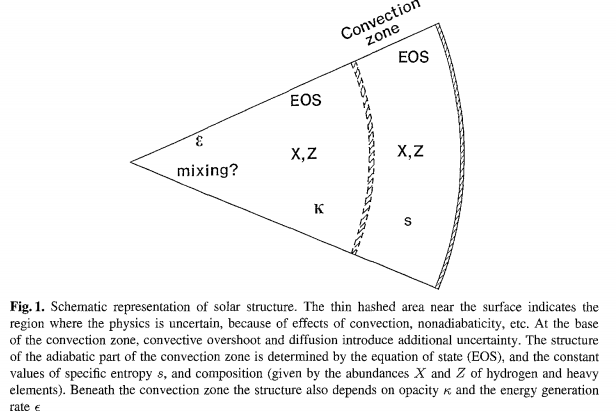
\includegraphics[width=(\textwidth),height=(\textheight-11mm),keepaspectratio]{SchemSstructure}
\caption{struttura schematica sole}
\end{figure}

La luminosit\'a dipende fortemente dal valore di $Y_0$,  mentre il raggio da $\alpha$, parametro che regola l'efficienza del trasporto convettivo nella regione esterna caratterizzata fisicamente dall'entropia il cui valore \'e determinato, a meno di una costante additiva, dalla zona superadiabatica vicino alla superficie. Infatti, in un modello semplificato in cui si descrive la zona convettiva con stratificazione quasi-adiabatica tramite $P=K\rho\expy{\gamma}$, l'eccesso di entropia specifica tra la fotosfera e la parte quasi-adiabatica
\begin{equation}
\Delta S=\int_{\ln{P_{Ph}}}^{\ln{P^*}} c_P(\nabla-\nabla_a)\,d\ln{P}
\end{equation}
con $P^*$ tale che $\nabla-\nad{}\ll1$, parametrizza la variazione di $\rsun{}$ e della profondit\'a della zona convettiva, essendo $\delta\ln{K}\approx\frac{5}{3}\frac{\delta(\Delta s)}{c_P}$:
\begin{align}
&\frac{\delta R}{R}\approx 0.24\,\delta\ln{K}\approx-0.24\,\delta\ln{\alpha}\\
&\frac{\delta d_{cz}}{R}\approx-0.02\,\delta\ln{K}&\intertext{cio\'e la calibrazione del raggio influenza poco la profondit\'a della zona convettiva.}\nonumber
\end{align}
%\cite{chr97effects}
Scelgo $Y_0$ e $\alpha$ che forniscono luminosit\'a e raggio $\rsun{}=\SI{6.96e8}{\meter}$ attuali del Sole: risulta $\frac{R_b}{\rsun{}}\approx0.710$ e il valore di $Y_0=0.250$.

\clearpage

\subsection{Mean free path of plasma particles}

\cite{pit12kinetics}

\begin{definition}{Almost ideal plasma}
Suffiently rarefied to apply equation of transport to it.
\begin{equation*}
kT\gg \frac{e^2}{\overline{r}}\approx e^2n\expy{\frac{1}{3}}
\end{equation*}
\end{definition}

\begin{definition}{Debye length}
\begin{equation*}
\frac{1}{a^2}=(\frac{4\pi}{T})\sum_an_a(z_ae)^2
\end{equation*}
\end{definition}

Pg .184

\begin{usefull}{Ion-ion mean free path}
Ion-Ion collision mean free path
\begin{align*}
&l_i\approx \frac{T_i^2}{4\pi e^4 n L_i}\\
&L_i=\log{\frac{aT_i}{e^2}}&\intu{Coulomb logarithm\index{Coulomb logarithm}}\\
\end{align*}
\end{usefull}


\begin{usefull}{Transport coefficients}
Using kinetic theory of gas
\begin{itemize}
\item Electrical conductivity $\sigma$. 
\begin{align*}
&v\approx\tau e\frac{E}{m},\ j\approx env\\
&\sigma\approx\frac{e^2n\tau}{m}\approx\frac{e^2nl}{mv_T}\\
&\sigma\approx \frac{T_e\expy{\frac{3}{2}}}{e^2m\expy{\frac{1}{2}}L_e}\\
\end{align*}

\item Therma conductivity: electron play the main part.
\begin{align*}
&\kappa\approx n_el_ev_{T_e}c_e\, c_e\approx1
&\kappa\approx\frac{T_e\expy{\frac{5}{2}}}{e^4m\expy{\frac{1}{2}}L_e}
\end{align*}

\item the viscosity is mainly due to ions since they carry most of the momentum; moreover is almost unchanged after collision with electron. we consider ii only:
\begin{align*}
&\eta\approx n_iMl_iv_{T_i}\\
&\eta\approx M\expy{\frac{1}{2}}\frac{T_e\expy{\frac{5}{2}}}{e^4L_i}
\end{align*}
\end{itemize}

\end{usefull}

\subsection{Processi di diffusione.}

Nei modelli solari standard i processi di diffusione non sono generalmente inclusi ma modelli con diffusione forniscono risultati pi\'u aderenti alle frequenze osservate.


I processi di diffusione inglobano diversi effetti: la gravit\'a tende a concentrare gli elementi pi\'u pesanti verso il centro, il campo elettrico mantiene gli elettroni ancorati ai nuclei, la diffusione termica concentra le particelle pi\'u cariche e pi\'u pesanti nelle zone pi\'u calde, mentre la diffusione proporzionale al gradiente di concentrazione $C_s=\frac{n_s}{n_e}$ diminuisce le disomogeneit\'a.

Definisco il parametro di plasma per specie s,t:
\begin{align}
&\Lambda_{st}=\frac{3KTr_D}{|e_se_t|}\\
&r_D=\sqrt{\frac{KT}{4\pi\sum_sn_se_s^2}}
\end{align}
che indica il grado di interazione tra le due specie.


\begin{todo}{Inhomogeneities nuil up base convection zone.}
In models that incorporate the diffusion and
gravitational settling of helium and heavy-elements, the abundances of these
elements build up below the convection-zone base.
\end{todo}

Processi di diffusione modificano l'abbondanza degli elementi, il peso molecolare medio e l'opacit\'a. Sebbene il tempo caratteristico per percorre un raggio solare si relativamente lungo $\tau_{diff}\approx\SI{6e13}{\year}$ i processi di diffusione sono apprezzabili rispetto SSM con/senza, in particolare:

\begin{itemize}
    \item Diminuzione della profondit\'a della zona convettiva circa $2\%$.
    \item Abbondanza He iniziale $+0.4\%$ nei modelli con diffusione.
    \item La diminuzione di He rispetto ad H comporta un'aumento delle stime di Z rispetto ad H del $3\%$.
\end{itemize}

Le differenze nella struttura interna hanno effetto sulle frequenze di oscillazione predette per circa \SIrange{1}{5}{\micro\hertz}.

\begin{figure}[!ht]
\centering
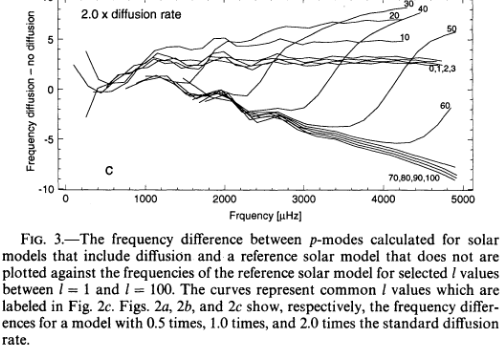
\includegraphics[width=(\textwidth),height=(\textheight-11mm),keepaspectratio]{diffusionDnu}
\caption{Differneza nelle frequenze previste.}
\end{figure}

Differenze nelle frequenze calcolate per modelli con/senza diffusione:
\begin{itemize}
    \item Effetto della diffusione sui modi p \'e proporzionale al coefficiente di diffusione.
    \item Aumente frequenze modi p di basso grado nell'intero range \SIrange{1000}{4500}{\micro\hertz}.
    \item Diminuisce di \SIrange{1}{5}{\micro\hertz} le frequenze dei modi p di alto grado.
    \item Le differenze nei modi p di grado intermedio son determinate dal grado di penetrazione oltre il fondo della zona convettiva.
\end{itemize}

\clearpage

\subsection{Helioseismically constrained model}

\subsubsection{Helioseismology, solar models and NF (innocenti97)}

Il valore dell atemperatura centrale \'e determinato da opacit\'a $\kappa$ e $\frac{Z}{X}$: we allow that both are rescaled by multiplicative factor with respect to value used in SSM, these scaling factors then determined by helioseismic constraints on convective envelope.

\subsubsection{Solar model from helioseismology (Dziembowski90)}

Having determined $P(r)$ and $\rho(r)$ in the Sun's interior we can attemnpt to construct a comlpete helioseismologica model assuming

\begin{itemize}
    \item thermal equilibrium
    \item $T(\rho,P,X)$
    \item opacity in the form $\kappa(\rho,T,X)$
    \item Nuclear energy generation rate $\epsilon(\rho,T,X)$.
    
    But in outer part of solar core $He\indices{^3}$ content cannot be determinedfrom equilibrium condition.
\end{itemize}

\chapter{Equazione di stato}
\PartialToc

Le correzioni alle grandezze termodinamiche si esprimono tramite $x=\frac{l_L}{r_D}$ con

\begin{equation*}
r_D=\sqrt{\frac{KT}{4\pi\sum_sn_se_s^2}},\ l_L=\frac{e^2}{KT}
\end{equation*}

e in particolare la correzione alla pressione risulta negativa:

\begin{align*}
&P_{ES}=\frac{1}{3}U_{ES}<0\shortintertext{con}\nonumber\\
&U_{ES}=\sum eZ\overline{n}_ZV_{ES}=-\frac{e^3(\sum Z^2\overline{n}_Z)\expy{\frac{3}{2}}}{2(4\pi\epsilon_0)(\epsilon_0KT)\expy{\frac{1}{2}}}
\end{align*}

Il contributo degli elettroni, detta $n_e$ la densit\'a numerica, $\psi=\frac{KT}{KT_F}\approx\num{3e-6}T(\frac{\mu_e}{\rho})\expy{\frac{2}{3}}$ il parametro di degenerazione e $u_k$ energia cinetica dell'elettrone, \'e determinato da
\begin{align}
&\rho N_A\frac{1+X}{2}=\intzi{}\frac{8\pi p^2\,dp}{h^3(\exp{\frac{u_k}{KT}-\psi}+1)},\ \beta P-\rho\gasconstant{}(X+\frac{Y}{4}+\frac{Z}{\exv{A_Z}})=\frac{1}{3}\intzi{}pn_e\TDy{p}{u_k}\,dp\shortintertext{dove ho introdotto il peso atomico medio per elettrone libero (ionizzato) $\mu_e$ con}\nonumber
&\frac{1}{\mu_e}\approx X+\frac{1}{2}Y+\frac{1}{2}(1-X-Y)=\frac{1+X}{2}
\end{align}

\stopcontents[chapters]

\end{document}

%\documentclass[../main.tex]{subfiles}

\begin{document}

\chapter{Oscillazioni lineari adiabatiche. Modi di oscillazione.}
\PartialToc


\section{Per punti.}

\tool{
\begin{itemize}
    
    \item Perturbazioni: reazione del sistema: oscillazioni.
    
    \item Relazioni perturbazioni vs Langrangiana (Tolsoy): in entrambe introduco la perturbazione della posizione $\Lvar{\vec{\xi}}$, ma tolsoy gi\'a ignora la perturbazione di $g$.
    \item Adiabatic approximation: dalsgaard, stellar oscillation pg.47: why we can neglect heating term in energy equation.
    
    \item Nel caso di onde puramente acustiche
    \begin{align*}
    &\PtwoDy{t}{\rho'}=-v_S^2\nabla^2\rho'\intertext{equazione d'onda per la propagazione della perturbazione}\\
    &v_S=\sqrt{\frac{\Gamma_{1,0}P_0}{\rho_0}}&\intertext{adiabatic (Laplacian) sound speed.}
    \end{align*}

    Usando l'equazione di continuit\'a si vede che
    \begin{align*}
    &|\frac{\rho'}{\rho_0}|=\frac{v}{v_S}\\
    &|\frac{\rho'}{\rho_0}|\ll1\ \Rightarrow \ \frac{v}{v_S}\ll1
    \end{align*}
    La teoria lineare \'e valida finch\'e la velocit\'a delle fluttuazioni associata alle onde acustiche \'e minore rispetto alla velocit\'a del suono.
    Per l'equazione per la quantit\'a di moto linearizzata deve essere $\vec{c}\parallel \vec{k}$: la velocit\'a del fluido associato alle onde acustiche adiabatiche \'e parallela alla direzione di propagazione, sono ande di pressione.
    
    \item Forward problem: Matching accuracy of observations with accuracy of theoretical predictions.
    
    \item Metodo asintotico: varie approssimazioni. Accuratezza $10\%$. Le tecniche di inversione numerica hanno accuratezza \numrange{100}{1000} volte superiore ma dipende da un modello solare: dipendenza radiale dei coefficienti nelle equazioni delle oscillazioni.
    
    \item At observed solar frequencies the displacement at surface is approx. radial:
    
    \begin{equation*}
    \frac{\xi_h(R)}{\xi_r(R)}\approx\frac{GM}{R^3}\frac{L}{\omega^2}
    \end{equation*}
    
    \item L'approssimazione di Cowling \'e troppo grossolana se paragonata con l'accuratezza delle osservazioni \num{e-4}.
    (Vedi Robe68 JCD84)
    
    \item Confronto accuratezza asintotica vs numerica vs accuratezza osservazioni
    
    \item Procedure for determine n for computed modes of oscillation: Scufflaire 74, Osaki 75.
    
    \item Cowling approximation: System of equation of second order: Sturm-Liuville problem.
    \item Classification is invariant under continuus variation of equilibrium model: $\lambda=0$ Cowling approximation, $\lambda=1$ full case.
    
    \item Numerical inaccuracy: Van der raay, Palle roca cortes 1986.
    
    \item Mathematical classification often doesn't reflect the physical nature of the modes (Osaki75)
    
    \item Integrated energy: (relative) kinetic energy within a mode
    \begin{equation*}
    E_{n,l}=\frac{\int_0^R[\xi^2_r(r)+l(l+1)\xi_h^2(r)]\rho r^2\,dr}{4\pi M[\xi^2_r(R)+l(l+1)\xi_h^2(R)]}
    \end{equation*}
    
    \item dispersione energia del modo: effetti non adibatici (superficie), effetti non lineari (accoppiamento con altri modi, accoppiamento con flussi di materia)
    
    \item Trapping of modes.
    
    \item Reflection due to increase of $\omega_c$ in external layers before adiabatic approx break down: for what modes ??
    
    
    \item Identificazione dei modi: identificazione dei promontori nel diagramma \dgndi{} and of the lines in the power spectrum of the full disc oscillation signal.
    \item extrapolation to infinite number of grid points (shibahashi osaki 81)
    \item Pulsational unstable: self-excited oscillations.
    \item Eigenfrequencies for an infinite number of grid point is extrapolated $\nu_N=\nu_{\infty}+\frac{a}{N^2}$
    \item Forward problem: asymptotic expression for frequencies.
    \item dipendenza parametrica modello forward problem: asymptotic vs numerical.
\end{itemize}
}

In questa sezione descrivo le caratteristiche dei modi normali del Sole e come la struttura del interna del Sole influisce sulle frequenze.

Quando le frequenza sono molto grandi (per i modi p) o molto piccole (per i modi g) \'e possibile ricavare soluzioni analitiche approssimate delle equazioni delle oscillazioni. 

\section{Perturbazioni lineari adiabatiche.}

\subsection{Perturbatione dello stato di equilibrio.}

\begin{todo}{Cerca ampiezza media oscillazioni superficie ($\exv{v_{osc}}$)}
La piccola ampiezza delle oscillazioni giustifica l'uso solo del termine lineare dell'espansione.

\end{todo}

Descrivo le oscillazioni come piccole perturbazioni attorno allo stato di equilibrio stazionario (gli effetti non lineari sono dell'ordine di $\frac{v}{c_s}$ dove v \'e l'ampiezza dell'oscillazione):

\begin{align*}
&P(\vec{r},t)=P_0(\vec{r})+P'(\vec{r},t)&\intertext{$P'(\vec{r},t)$ \'e la perturbazione euleriana, quindi, detto $\delta\vec{\xi}$ lo spostamento della particella di fluido a causa della perturbazione}\\
&\Lvar{P(\vec{r})}=P(\vec{r}+\Lvar{\vec{\xi}})-P_0(\vec{r})=P'(\vec{r})+\Lvar{\vec{\xi}}\cdot\nabla P_0&\intertext{la velocit\'a dell'elemento di fluido dovuta alla perturbazione \'e}\\
&\vec{v}=\PDof{t}(\Lvar{\vec{\xi}})
\end{align*}

\begin{todo}{Particular solution/Perturbed solution}
Equations of conservation for stellar structure form a system of non-linear, partial differential equations. If an unperturbed solution is known we are often interested in finding another solution ''perturbed'' which differs only slightly from the unperturbed (we may think of the two solutions as representing possible future of the fluid differing from each others because of different initial conditions).

Expressing dependent variable of perturbed solutions as the sum of corr. dependent vars of unperturbed solution, neglecting all powers above the first and product of variations we obtain a system of partial differential equation whose solution gives the behaviour of the variation: the resulting set of equations is linear.

\end{todo}

Ricavo l'equazione del moto perturbato
\begin{align}
&\intertext{sostituisco nell'equazione del moto}
    &\rho\TDof{t}v\indices{_i}=\rho(\PDy{t}{v\indices{_i}}+v\indices{_j}\partial\indices{_j}v\indices{_i})=-\nabla P\indices{_i}+\rho\vec{g}\indices{_i}&\intertext{ le grandezze perturbate e sottraendo l'equazione statica ottengo}\nonumber\\
&\rho_0\PtwoDy{t}{\Lvar{\vec{\xi}}}=\rho_0\PDy{t}{\vec{v}}=-\nabla P'+\rho_0\vec{g}'+\rho'\vec{g}_0\label{eq:emper}\\
&\vec{g}'=-\nabla\Phi',\ \nabla^2\Phi'=4\pi G\rho'\nonumber
\end{align}

Analogamente per l'equazione di continuit\'a ottengo
\begin{equation}
\rho'+\div{(\rho_0\Lvar{\vec{\xi}})}=0\label{eq:contper}
\end{equation}

\subsection{Adiabatic approximation}

I tempi caratteristici per scambio di calore sono maggiori del periodo delle pulsazioni


\begin{align*}
&\TDy{t}{q}=\frac{1}{\rho(\Gamma_3-1)}(\TDy{t}{P}-\frac{\Gamma_1P}{\rho}\TDy{t}{\rho})=\epsilon-\frac{1}{\rho}\scap{\nabla}{F}&\intu{energy equation (rate heat gain/loss)}\\
&\frac{1}{\rho c_P}\nabla\cdot(\frac{4acT^3}{3\kappa\rho}\nabla T)\approx\frac{4acT^4}{3\kappa\rho^2c_PH}=\frac{T}{\tau_R}&\intertext{$\tau_R$ tempo scala radiativo, H lunghezza caratteristica, in cgs:}\\
&\tau_R=\num{e12}\frac{\kappa\rho^2H^2}{T^3}
\end{align*}

Per valori caratteristici solari ($\kappa=1$, $\rho=1$, $T=\num{e6}$, $H=\num{e10}$) ho $\tau_R\approx\SI{e7}{\year}\approx\tkh{}$, per valori caratteristici della zona convettiva ($\kappa=100$, $\rho=\num{e-5}$, $T=\num{e4}$, $H=\num{e9}$) ho $\tau_R\approx\SI{e3}{\year}\approx\tkh{}$.


In the inner part the nuclear term correspond to characteristic time $\tau_{\epsilon}\approx\frac{c_PT}{\epsilon}\approx\tkh{}$.

Confronto $\frac{T}{\tau_R}$, $\frac{T}{\tau_{\epsilon}}$ con $\TDy{t}{T}\approx\frac{T}{\Pi_{osc}}$ con $\Pi_{osc}\approx\si{\minute}-\si{\hour}$: heating term is generally very small compared with time derivative term.

Il moto di una elemento di fluido \'e descritto dalla relazione adiabatica


\begin{align*}
&\TDy{t}{P}=\frac{\Gamma_1P}{\rho}\TDy{t}{\rho}
\end{align*}

Approssimazione adiabatica non pi\'u valida vicino alla superficie solare dove i tempi per lo scambio di calore sono pi\'u brevi.

La condizione di perturbazione adiabatico linearizzata \'e
\begin{align}
&\PDy{t}{\Lvar{P}}-\frac{\Gamma_{1,0}P_0}{\rho_0}\PDy{t}{\Lvar{\rho}}=0\nonumber&\intertext{che integrata rispetto a t ed in funzione della variazione euleriana diventa}\nonumber\\
&P'+\Lvar{\vec{\xi}}\cdot\nabla P_0=\frac{\Gamma_{1,0}P_0}{\rho}(\rho'+\Lvar{\vec{\xi}}\cdot\nabla\rho_0)\label{eq:adper}
\end{align}

\subsection{Separazione variabili spaziali e temporali.}

Dall'equazione del moto \ref{eq:emper} si vede che
\begin{align*}
&\hat{r}\cdot(\rot{\PtwoDy{t}{\vec{\xi}}})=0&\intertext{cio\'e}\\
&\PDof{\theta}(\sin{\theta}\xi_{\phi})-\PDy{\phi}{\xi_{\theta}}=0&\intertext{quindi \'e possibile ricavare la componente tangenziale della perturbazione da una funzione scalare e dato che sono interessato alle oscillazioni }\\
&\vec{\xi}=\exp{i\omega t}(\xi_r(r),\xi_h(r)\PDof{\theta},\frac{\xi_h(r)}{\sin{\theta}}\PDof{\phi})Y_l^m(\theta,\phi)&\intertext{Ho introdotto le funzioni armoniche sferiche che soddisfano:}\\
&L^2Y_l^m=-\frac{1}{\sin{\theta}}\PDof{\theta}(\sin{\theta}\PDy{\theta}{Y_l^m})\\
&+\frac{1}{\sin^2{\theta}}\PtwoDy{\phi}{Y_l^m}=-r^2\nabla_h^2Y_l^m=l(l+1)Y_l^m
\end{align*}

La variazione euleriana di densit\'a, pressione, potenziale gravitazionale sono espressi
\begin{align*}
&(\rho_1,P_1,\Phi_1)=\exp{i\omega t}[\rho_1(r),P_1(r),\Phi_1(r)]Y_l^m
\end{align*}

\subsection{Frequenze di oscillazione discrete.}

Utilizzo l'equzione del moto ~\ref{eq:emper} e l'equazione di continui\'a~\ref{eq:contper} per eliminare $\xi_h(r)$ dall'equazione del moto
\begin{align}
&\frac{1}{r^2}\TDof{r}(r^2\xi_r)-\frac{\xi_rg}{c^2}+\frac{1}{\rho_0}(\frac{1}{c^2}-\frac{l(l+1)}{r^2\omega^2})P_1\nonumber\\
&-\frac{l(l+1)}{r^2\omega^2}\Phi_1=0\nonumber\\
&\frac{1}{\rho_0}(\TDof{r}+\frac{g}{c^2})P_1-(\omega^2-N^2)\xi_r+\TDy{r}{\Phi_1}=0\label{eq:eigenomega}\\
&\frac{1}{r^2}\TDof{r}(r^2\TDy{r}{\Phi_1})-\frac{l(l+1)}{r^2}\Phi_1-\frac{4\pi G\rho_0}{g}N^2\xi_r\nonumber\\
&-\frac{4\pi G}{c^2}P_1=0\nonumber
\end{align}

ho definito $N^2=g(\frac{1}{\Gamma_1P_0}\TDy{r}{P_0}-\frac{1}{\rho_0}\TDy{r}{\rho_0})$ e $S_l^2=\frac{l(l+1)c^2}{r^2}\approx k_h^2c^2$ con

\begin{align*}
&g=-\frac{1}{\rho_0}\TDy{r}{P_0}\\
&c^2=\frac{\Gamma_1P_0}{\rho_0}
\end{align*}


Il sistema di equazione ~\ref{eq:eigenomega} ha soluzione con le opportune equazioni al contorno per un insieme discreto di valori delle frequenze $\omega_{nlm}$, l'ordine angolare non compare nelle equazioni quindi gli autovalori $\omega_{nlm}$ sono $2l+1$ degeneri.

\subsection{Condizioni al contorno}

Abbiamo bisogno di 4 condizioni

\begin{itemize}
\item Due condizioni per $r=0$ punto regolare: le perturbazioni sono non singolari al centro del Sole, $r=0$.

\begin{equation*}
P'=0,\ \Phi'=0
\end{equation*}

Expansion near zero of solutions

\begin{align*}
&(l\neq0):\ \xi_r\propto r\expy{l-1};\ (l=0):\ \xi_r\propto r\\
&P',\ \Phi'\propto r^l
\end{align*}

\item Alla superficie solare richiediamo la continuit\'a di $\Lvar{\nabla\Phi}$ e che non si abbia dispersione verso l'esterno.

Outside the star $\rho'=0$ and Poisson equation can be solved by solution vanishing at infinity $\Phi'=Ar\expy{-l-1}$:
\begin{equation*}
\TDy{r}{\Phi'}+\frac{l+1}{r}\Phi'=0,\ r=\rsun{}    
\end{equation*}

The second condition depends on treatment of stellar atmosphere (Vedi chap 5 of lecture note on stellar oscillations: pg 103, (5.50)). It's reasonable that the boundary is free, no force acts on it: the star can be considered an isolated system. This is equivalent to requiring pressure constant at perturbed surface.

\begin{align*}
&\Lvar{P}=P'+\xi_r\TDy{r}{P}=0
\end{align*}

\end{itemize}

\subsection{Variabili adimensionali.}

Introduco le variabili adimensionali, che caratterizzano la perturbazione

\begin{align*}
&\eta_1=\frac{1}{r}\xi_r\\
&\eta_2=\frac{1}{gr}(\frac{P'}{\rho}+\Phi')\\
&\eta_3=\frac{1}{gr}\Phi'\\
&\eta_4=\frac{1}{g}\PDy{r}{\Phi'}\\
&\eta_i=\eta_i(r)Y_l^m(\theta,\phi)\exp{i\omega t}
\end{align*}

e riscrivo l'equazione del moto

\begin{equation*}
-\frac{\omega^2}{g}\vec{\xi}=[W(\eta_1-\eta_2+\eta_3)+(1-U)\eta_2]\hat{r}-r\nabla\eta_2
\end{equation*}

in funzione delle grandezze $U,V,W$ che caratterizzano lo stato di equilibrio del Sole

\begin{align*}
&U=\frac{r}{m}\PDy{r}{m}=\frac{1}{g}\PDy{r}{(gr)}\\
&V=-\frac{r}{P}\PDy{r}{P}=\frac{g\rho r}{P}\\
&W=\frac{r}{\rho}\PDy{r}{\rho}-\frac{r}{P\gamma_{Ad}}\PDy{r}{P}
\end{align*}

posto $\gamma_{ad}=\Dcvar{\TDly{\rho}{P}}{ad}=\Gamma_1$

La parte tangenziale dell'equazione del moto
\begin{align*}
&\frac{\omega^2}{g}\xi_{\theta}=\PDy{\theta}{\eta_2},\ &\frac{\omega^2}{g}\xi_{\phi}=\frac{1}{\sin{\theta}}\PDy{\phi}{\eta_2}
\end{align*}
sostituita nell'equazione di continuit\'a ($\scap{\nabla}{\xi}$), definita la frequenza adimensionale 
\begin{equation*}
\frac{\omega^2r}{g}=C\sigma^2:\ \sigma^2=\omega^2\frac{R^3}{GM}
\end{equation*}

permette di eliminare la dipendenza dalle variabili angolari
\begin{align*}
&r\PDy{r}{\eta_1(r)}=(3-\frac{V}{\gamma_{Ad}})\eta_1(r)+[\frac{l(l+1)}{C\sigma^2}\\
&+\frac{V}{\gamma_{Ad}}]\eta_2(r)-\frac{V}{\gamma_{Ad}}\eta_3
\end{align*}

mentre la parte radiale dell'equazione del moto

\begin{equation*}
r\PDy{r}{\eta_2(r)}=(W+C\sigma^2)\eta_1(r)+(1-U-W)\eta_2(r)+W\eta_3
\end{equation*}

dalla definizione di $\eta_3$

\begin{equation*}
r\PDy{r}{\eta_3}=(1-U)\eta_3(r)+\eta_4
\end{equation*}

infine l'equazione di Poisson \'e equivalente a
\begin{equation*}
r\PDy{r}{\eta_4}=-UW\eta_1+\frac{UV}{\gamma_{Ad}}\eta_2+[l(l+1)-\frac{UV}{\gamma_{Ad}}]\eta_3-U\eta_4
\end{equation*}



Abbiamo ottenuto quattro equazioni differenziali a coefficienti reali che dipendono dallo stato di equilibrio del modello stellare per le variabili adimensionali $\eta_i(r)$: un problema agli autovalori per $\sigma^2$, si pu\'o vedere che \'e autoaggiunto e quindi le autofunzioni corrispondenti ad autovalori diversi sono ortogonali: gli autovalori sono reali quindi posso avere un comportamento oscillante nel caso di stabilit\'a o esponenziale nel caso instabile.

Il sistema non dipende da m: le soluzioni sono $(2l+1)$ volte degeneri: la degenerazione \'e rimossa dalla rotazione ($\frac{\Omega}{\omega}\approx\num{e-4}$) o effetti gravitazionali di altri corpi.


\section{Stabilit\'a dei modi di oscillazione.}

\begin{todo}{Stabilit\'a oscillazioni nonradiali adiabatiche}

\end{todo}



\end{document}
%\documentclass[../main.tex]{subfiles}

\begin{document}

\section{Propriet\'a generali delle oscillazioni adiabatiche.}

\begin{todo}{Frequenza di \bv{}.}
qui o nella sottosezione precedente??
Kippenhan: 40.3, eigenspectra
Dalsgaard: notes 5.3Pg 83-
\end{todo}

\begin{comment}
\begin{figure}[!ht]
\centering
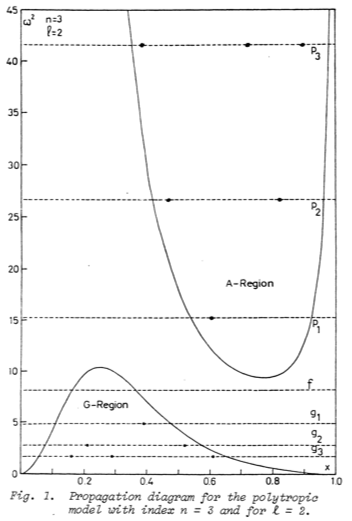
\includegraphics[width=\textwidth, height=0.9\textheight,keepaspectratio]{propagationAG}
\caption{Regioni di propagazione.}
\end{figure}
\end{comment}

\begin{todo}{dalsgaard 2005}
homology argument: scaling factor $\sqrt{GM}$
\end{todo}


\begin{todo}{Soluzioni numeriche e comportamentpo asintotico}
La soluzione numerica \'e dipendente dal modello di equilibrio: per il modello stellare $M4K$ viene riportata un precisione di $\SI{0.02}{\micro\hertz}$ (accuratezza \num{e-5}), mentre differenti valori della costante G fra quelli usati in letteratura risultano in differenze nelle frequenze calcolate di \numrange{-0.35}{-0.08}\si{\micro\hertz}, maggiori di quelle che risultano da differenti schemi di integrazione numerica.
\end{todo}

\begin{todo}{Numerical technique}
Inter-comparison of the g-, f- and p-modes calculated using different oscillation codes for a given stellar model

\end{todo}

\begin{todo}{Continous variation of parameter}
Problems in cowling vs full
\end{todo}

La soluzione numerica delle equazioni \eqref{eq:eigenomega}


\begin{comment}
\begin{figure}[!ht]
\centering
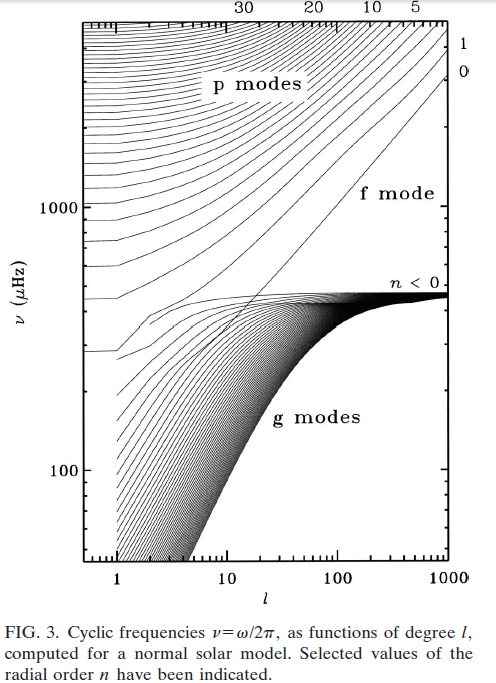
\includegraphics[width=\textwidth, height=0.9\textheight,keepaspectratio]{omega-l}
\caption{Modi di oscillazion. plot omega vs l..}
\end{figure}
\end{comment}

mostra due differenti comportamenti. Uso l'approssimazione asintotica per determinare la natura delle oscillazioni nelle due zone.

\clearpage

\subsection{Comportamento asintotico}


Per determinare la struttura dello spettro delle oscillazioni introduciamo l'approssimazione di Cowling (\cite{cow41oscillations}) cio\'e trascuriamo la perturbazione del potenziale gravitazionale. Quindi il sistema si riduce al secondo ordine

\begin{align}
&\frac{1}{r^2}\TDof{r}(r^2\xi_r)-\frac{\xi_rg}{c^2}+\frac{1}{\rho_0}(\frac{1}{c^2}-\frac{l(l+1)}{r^2\omega^2})P_1=0\label{eq:cowosc}\\
&\frac{1}{\rho_0}(\TDof{r}+\frac{g}{c^2})P_1-(\omega^2-N^2)\xi_r=0\nonumber
\end{align}

Considero i limiti asintotici di alte e basse frequenze: in entrambi ottengo un problema del tipo di Sturm-Liuville

\begin{todo}{Sturm-Liouville theory}
%https://en.wikipedia.org/wiki/Sturm%E2%80%93Liouville_theory
\end{todo}

\begin{todo}{Modi stabili/instabili}
Cox ??
\end{todo}

\begin{itemize}
\item Per $\omega\to\infty$:

Lo spettro \'e discreto con punto di accumulazione a $\omega=\infty$.
Le oscillazioni sono prodotte da onde acustiche in cui la forza dominante \'e fornita dalla pressione, chiamati modi p, ordinati in base al numero di zeri di $\xi_r$ fra il centro e la superficie. I modi p sono stabili.

\item Per $\omega\to0$:

Lo spettro \'e discreto con punto di accumulazione a $\omega=0$.
Il moto \'e determinato dalla forza di gravit\'a, chiamati modi g (ordinati secondo il numero di nodi radiali). La stabilit\'a dei modi g \'e detrminata dalla stabilit\'a convettiva: dato che $\omega^2_{Ad}=-grW$ il criterio di instabilit\'a convettiva si traduce in $rW>0$. Se $W<0$ in tutta la stella tutti i modi g sono stabili ($g_+$), se esistono zone in cui $W>0$ esistono anche modi g instabili ($g_-$).
\end{itemize}

Lo spettro solare \'e la combinazione dei modi parziali precedenti; il modo f separa  i modi g e p: non ha nodi in direzione radiale.

\subsection{Relazione di dispersione per i modi gravo-acustici.}

Approssimo il comportamento spaziale delle oscillazioni con quello di onda piana
\begin{align*}
&\vec{\xi}\propto\exp{i\scap{k}{x}},\ \vec{k}=k_r\hat{r}+\vec{k}_h\\
&S_l^2=\frac{l(l+1)c^2}{r^2}\approx k_h^2c^2
\end{align*}
e i coefficienti delle equazioni \ref{eq:cowosc} costanti ( approssimazione valida se la lunghezza d'onda delle perturbazioni \'e molto minore della scala caratteristica di variazione dei coefficienti).

\begin{todo}{Per poter parlare di onde}
Per poter parlare di onde devo assumere che la variazione di $P_0$ e $\rho_0$ abbiano lunghezze caratteristiche maggiori delle lunghezze di interesse (short-wave acustic):
\begin{align*}
&\PtwoDy{t}{\rho'}=-v_S^2\nabla^2\rho'\intertext{equazione d'onda per la propagazione della perturbazione}\\
&v_S=\sqrt{\frac{\Gamma_{1,0}P_0}{\rho_0}}&\intertext{adiabatic (Laplacian) sound speed.}
\end{align*}



Usando l'equazione di continuit\'a si vede che
\begin{align*}
&|\frac{\rho'}{\rho_0}|=\frac{v}{v_S}\\
&|\frac{\rho'}{\rho_0}|\ll1\ \Rightarrow \ \frac{v}{v_S}\ll1
\end{align*}
La teoria lineare \'e valida finch\'e la velocit\'a delle fluttuazioni associata alle onde acustiche \'e minore rispetto alla velocit\'a del suono.
Per l'equazione per la quantit\'a di moto linearizzata deve essere $\vec{c}\parallel \vec{k}$: la velocit\'a del fluido associato alle onde acustiche adiabatiche \'e parallela alla direzione di propagazione, pressure force supply the restoring force.

\end{todo}

Manipolando il sistema \ref{eq:cowosc} inserendo perturbazioni della forma (conservazione energia) $\xi_r\propto\rho_0\expy{-\frac{1}{2}}\exp{ik_rr}$, $P_1\propto\rho_0\expy{\frac{1}{2}}\exp{ik_rr}$:

\begin{align*}
&\frac{1}{r^2}\TDof{r}(r^2\xi_r)-\frac{\xi_rg}{c^2}+\frac{1}{\rho_0}(\frac{1}{c^2}-\frac{l(l+1)}{r^2\omega^2})P_1=0\\
&\frac{1}{\rho_0}(\TDof{r}+\frac{g}{c^2})P_1-(\omega^2-N^2)\xi_r=0\\
\\
&\xi_r=\frac{1}{(\omega^2-N^2)}[\frac{1}{\rho_0}(\TDof{r}+\frac{g}{c^2})]P_1\\
&\TDof{r}\xi_r=-\frac{2}{r}\xi_r+\frac{\xi_rg}{c^2}+\frac{1}{\rho_0}(\frac{1}{c^2}+\frac{l(l+1)}{r^2\omega^2})P_1\\
\\
&\TDof{r} \frac{1}{\rho_0}(\TDof{r}+\TDof{r} \frac{g}{c^2})P_1-(\omega^2-N^2)\TDof{r} \xi_r=0
\end{align*}

\begin{todo}{relazione dispersione stix pg 156 (5.33)}

Gough pg 792 eq 25-26

\end{todo}

Se considero $g$, $N$ e $c$ lentamente variabili rispetto alla lunghezza d'onda delle perturbazioni lo stesso vale per la lunghezza caratteristica della densit\'a $H=-\frac{\rho_0}{\TDy{r}{\rho_0}}=(\frac{g}{c^2}+\frac{N^2}{g})\expy{-1}$ e la frequenza di taglio acustica $\omega_A=\frac{c}{2H}$. Scrivo la relazione di dispersione

\begin{align}
&k_r^2=\frac{\omega^2-\omega_A^2}{c^2}+S_l\frac{N^2-\omega^2}{c^2\omega^2}\label{eq:localdispersion}\\
&=\frac{\omega^2}{c^2}(1-\frac{\omega_{l,+}^2}{\omega^2})(1-\frac{\omega_{l,-}^2}{\omega^2})\nonumber
\end{align}

\begin{comment}
\begin{figure}[!ht]
\centering
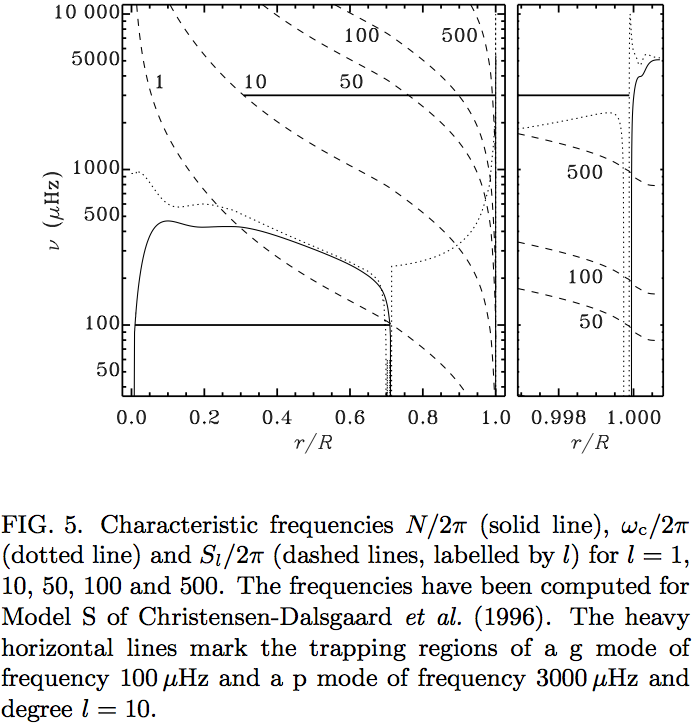
\includegraphics[width=\textwidth, height=0.9\textheight,keepaspectratio]{freqcaratt}
\caption{Frequenze caratteristiche.}
\label{fig:freqcaratt}
\end{figure}
\end{comment}

\clearpage


\section{Regioni di propagazione.}

\begin{comment}
\begin{figure}[!ht]
\centering
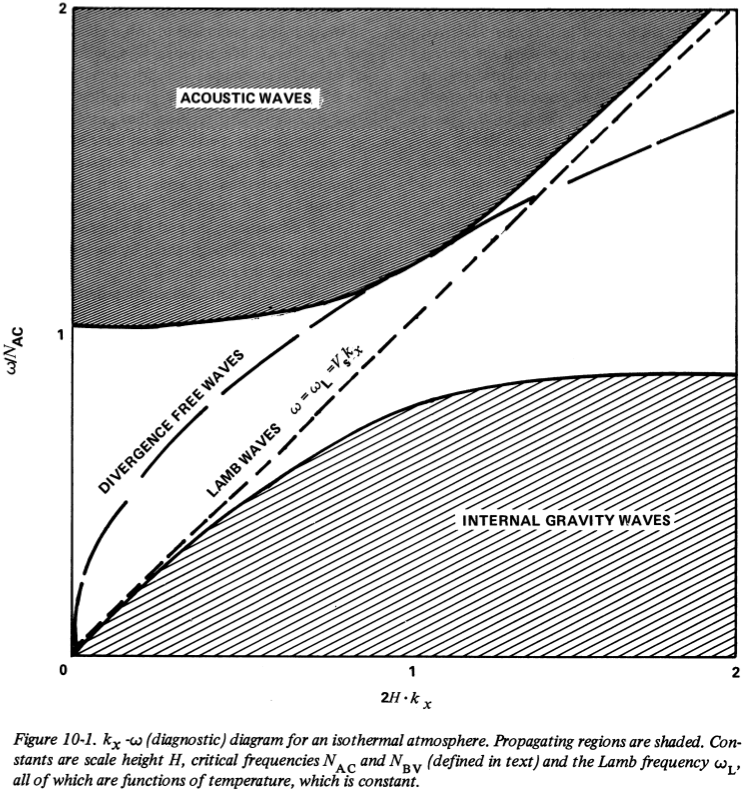
\includegraphics[width=\textwidth, height=0.8\textheight,keepaspectratio]{khomeagisot}
\caption{Diagramma frequenza numero d'onda orizzontale per atmosfera isoterma.}
\label{fig:khomeagisot}
\end{figure}

\begin{figure}[!ht]
\centering
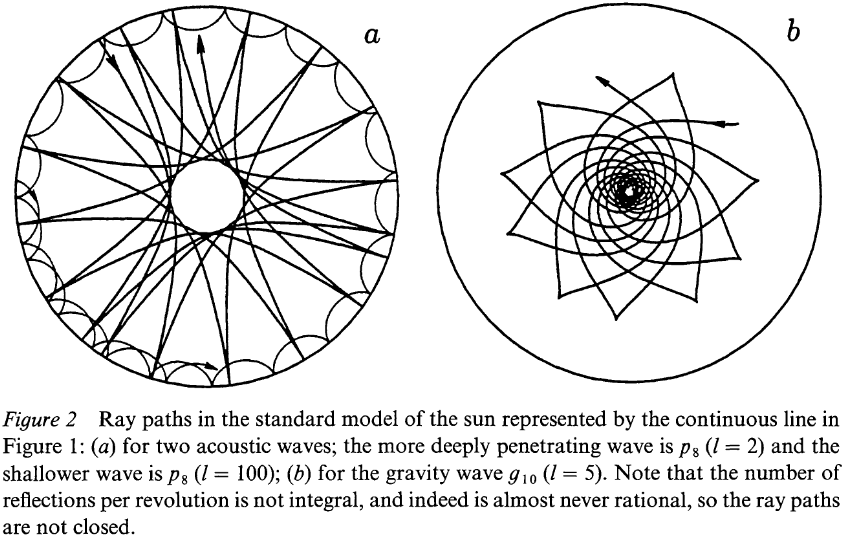
\includegraphics[width=0.9\textwidth, height=\textheight,keepaspectratio]{pgmodesC}
\caption{Cavit\'a risonanti per modi p e g.}
\label{fig:propagationAG}
\end{figure}
\end{comment}

Il comportamento oscillatorio richiede $k_r^2>0$.

I punti di inversione per le onde acustiche sono definiti da 
\begin{align*}
    &\omega^2=\frac{l(l+1)c}{r^2}&\intertext{large $k_hH$}\\
    &\omega=\omega_A&\intertext{small $k_hH$}
\end{align*}

per i modi g da
\begin{align*}
    &\omega=N&\intertext{large $k_hH$.}
    &\omega=(\frac{\omega_A}{N})ck_h&\intertext{small $K_hH$.}
\end{align*}

\'E possibile analizzare tramite metodo  JWKB il sistema di equazioni delle oscillazioni del secondo ordine in approssimazione di Cowling, previa oppurtuna trasformazione, da cui si ottiene la relazione valida per i modi
\begin{equation}\label{eq:jwkb}
\omega\int_{r_1}^{r_2}[1-\frac{\omega_A^2}{\omega^2}-\frac{S_l^2}{\omega^2}(1-\frac{N^2}{\omega^2})]\expy{\frac{1}{2}}\frac{dr}{c}\approx\pi(n-\frac{1}{2})
\end{equation}
dove $r_1$ e $r_2$ sono due zeri consecutivi del numero d'onda radiale e l'integrazione \'e in una regione di propagazione. Nel caso dei modi p e assumendo $S_l\ll\omega$ vicino al punto di inversione superiore ho

\begin{equation}\label{eq:jwkbmodep}
\omega\int_{r_1}^{r_2}[1-\frac{S_l^2}{\omega^2}]\expy{\frac{1}{2}}\frac{dr}{c}\approx\pi(n-\alpha{\omega})
\end{equation}

\clearpage

\subsection{Cavit\'a acustiche.}
Per grandi $\omega$ ~\ref{eq:localdispersion} si riduce alla relazione di dispersione acustica 

\begin{equation*}
\omega^2=c^2(k_r^2+k_h^2)
\end{equation*}


Posso ricavare il raggio di inversione del moto in direzione radiale $k_r=0$ dalla relazione di dispersione per onde onde acustiche, da cui segue
\begin{equation}
\frac{c(r_i)}{r_i}=\frac{\omega}{l(l+1)}
\end{equation}

Maggiore \'e il grado l (piccolo $\lambda_h$) meno profonda \'e la cavit\'a: sono riflesse verso la superfice quando la velocit\'a del suono \'e aumentata fino alla loro velocit\'a di fase orizzontale; la profondit\'a della cavit\'a acustica varia con il variare della scala orizzontale dell'onda. (Top  convection zone down to the level at which refraction due to sound speed increasing $c\propto\sqrt{T}$ turn the wave around when $c=\frac{\omega}{k_h}$)

Stima profondit\'a cavit\'a acustica
\begin{align*}
    &T=\Dcvar{\TDy{z}{T}}{Ad}\delta&\intu{$\delta$ \'e la profondit\'a sotto la fotosfera}\\
    &T=\Dcvar{\TDy{z}{T}}{Ad}=\frac{T}{P}\TDly{P}{T}|_{Ad}\TDy{z}{P}=\frac{\gamma-1}{\gamma R}g=\frac{g}{c_P}\\
    &c^2=(\gamma-1)g\delta&\intertext{da $c=\frac{\omega}{k_h}$ segue:}\\
    &\delta=\frac{\omega^2}{k_h^2(\gamma-1)g}
\end{align*}
minore la lunghezza d'onda orizzontale pi\'u sottile la cavit\'a.

Vicino alla superficie l'efficienza della convezione diminuisce, il gradiente di temperatura diventa fortemente sopra-adiabatico e la fraquenza critica $\omega_A$ aumenta notevolmente: le onde acustiche con periodo attorno ai 5-min diventano evanescenti in poche scale di altezza: l'inizio della zona convettiva \'e uno specchio a larga banda per onde acustiche. 

Duvall82

In un grafico $\frac{\omega}{k_h}$ vs $\frac{\pi(n+\alpha)}{\omega}$ i modi p sono rappresentati da un'unica curva. Se considero la differenza di fase
\begin{align}\label{eq:duvall}
&\Delta\phi=\int_{r_t}^{\rsun{}}k_r\,dr=\int_{r_t}^{\rsun{}}(\frac{1}{c^2}-\frac{l(l+1)}{r^2\omega^2})\expy{\frac{1}{2}}\,dr\\
&=F(\frac{\omega}{L})\\
&\Delta\phi=\pi(n+\alpha)
\end{align}
tra i bordi interno ed esterno della cavit\'a acustica per un modo di oscillazione $\Delta\phi=\pi(n+\alpha)$ la costante $\alpha$ \'e necessaria dato che i bordi non sono rigidi.
L'integrale risulta funzione di $\frac{\omega}{k_h}$. 

\begin{comment}
\begin{figure}[!ht]
\centering
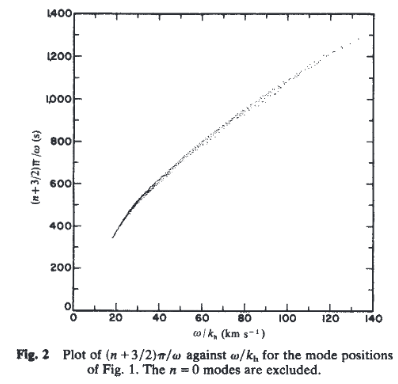
\includegraphics[width=\textwidth, height=0.9\textheight,keepaspectratio]{Duvall}
\caption{Legge di Duvall.}
\end{figure}
\end{comment}

\clearpage

\subsection{Cavit\'a risonanti per modi g.}

Nella parte a basse frequenze dei modi g la relazione \ref{eq:localdispersion} si approssima, per $l\neq0$ con

\begin{equation*}
k_r^2=\frac{S_l^2}{c^2}(\frac{N^2}{\omega^2}-1)
\end{equation*}

La regione dei modi g ha come limite superiore N per grandi l, la linea $\omega=\frac{S_lN}{\omega_A}$.

Per i modi g le regioni di propagazione sono quelle per la frequenza \'e minore di entrambi $N$ e $ck_h$.

La struttura degli strati esterni del sole \'e dominata dalla ionizzazione di H e He con conseguente aumento dell'opacit\'a e quindi del gradiente di temperatura in equilibrio radiativo e il calore specifico: il gradiente di temperatura critico per instabilit\'a convettiva $\frac{g}{c_P}$ diminuisce. In questa regione il gradiente di temperatura \'e debolmente super-adiabatico, $N^2<0$: la zona convettiva costituisce una barriera per le onde di gravit\'a interne.

Le onde di gravit\'a sono presenti nelle regioni in cui il gas \'e neutro o completamente ionizzato ($N^2$ grande) e sono riflesse in regioni dove $N$ \'e piccolo o immaginario: ionizzazione parziale, instabilit\'a convettiva, centro del Sole.

Ho cavit\'a risonanti per modi g:
\begin{itemize}
    \item Core radiativo.
    
    Tra la la parte centrale dove $g\to0$ e il fondo della zona convettiva dove $N^2<0$.
    \item Atmosfera.
    
    $N$ ha un massimo in coincidenza del punto $T_m$ nella cromosfera: modi g confinati tra zona convettiva e cromosfera ($\Pi\approx\numrange{180}{800}\si{\second}$).
\end{itemize}


\section{Analisi asintotica}

\begin{todo}{Analisi asintotica}
Vedi stix 5.3??

Heliosismic inference: observed vs predicted frequencies (Simple models and analytic (asyntotic) formula).
\end{todo}

\subsection{JWKB analysis}

\begin{todo}{cos'\'e l'analisi asintotica}
Vedi articolo gough07
\end{todo}

Nell'analisi tramite JWKB si tiene conto del fatto che le oscillazioni non sono puramente acustiche e le propriet\'a del gas non sono omogenee.

I modi osservati sono di alto ordine radiale o grado angolare: uso l'approssimazione di Cowling (ignoro la perturbazione al potenziale gravitazionale $\Phi'$).

\begin{align*}
&\omega\int_{r_1}^{r_2}\sqrt{1-\frac{\omega_c^2}{\omega^2}-\frac{S_l^2}{\omega^2}(1-\frac{N^2}{\omega^2})}\,\frac{dr}{c}\approx\pi(n-\frac{1}{2})\\
&\omega_c=\frac{c^2}{4H^2}(1-2\TDy{r}{H})\\
&H=-(\TDy{r}{\ln{\rho}})\expy{-1}
\end{align*}

\subsection{Asymptotic properties of p modes}

Posso trascurare N e, eccetto vicino alla superficie, $\omega_c\ll\omega$, mentr vicino alla superficie $S_l\ll\omega$ for small/moderate l.

\begin{align*}
&\omega\int_{r_1}^{r_2}\sqrt{1-\frac{\omega_c^2}{\omega^2}-\frac{S_l^2}{\omega^2}}\,\frac{dr}{c}\approx\pi(n-\frac{1}{2})&\intertext{where $r_1=r_t$, $r_2=R_t$. With help of our assumption we can expand the integral and, introducing the function $\alpha(\omega)$ depending only on frequency and near surface behaviour of $\omega_c$.}
\end{align*}

For low degree modes we use the fact that integrand differs from 1 only close to lower turning point close to center for low order mode ($F(w)\approx\int_0^R\frac{dr}{c}-w\expy{-1}\frac{\pi}{2}$)

\begin{align*}
&\nu_{nl}=\frac{\omega_{nl}}{2\pi}\approx(n+\frac{l}{2}+\frac{1}{4}+\alpha)\Delta\nu\\
&\Delta\nu=[2\int_0^R\frac{dr}{c}]\expy{-1}&\intu{is the inverse of twice travel time center/surface. This equation predict uniform spacing in n of frequency of low degree modes (claverie79)}
\end{align*}

Deviazioni da questa legge hanno potenziale diagnostico per la parte interna, infatti estendendo l'espansione di

\begin{equation*}
F(w)=\int_{r_t}^R\sqrt{1-\frac{c^2}{w^2r^2}}\,\frac{dr}{c}
\end{equation*}

fino al termine dipendente dalla variazione di c:

\begin{align*}
d_{nl}=\nu_{nl}-\nu_{n-1,l+2}\approx-(4l+6)\frac{\Delta\nu}{4\pi^2\nu_{nl}}\int_0^R\TDy{r}{c}\,\frac{dr}{c}&\intertext{sound speed is reduced as $\mu$ increases with H to He conversion as star ages: as a result $d_{nl}$ is reduced providing measure of evolutionary state of stars}
\end{align*}

\subsection{Asymptotic g modes}

In inner domain an expansion in terms of $\frac{\omega^2}{S_l^2}$ is possible, while $\frac{\omega^2}{N^2}$ serves as small expansion parameter in outer domain containing the surface, additional domains have to be considered for zeros of $N^2$

For the Sun we have $N^2(r_v)=0$ where $r_v$ marks lower bound of convection zone, matching the respective expansion we have in first order
\begin{align*}
&T_{n,l}=\frac{2\pi^2(n+\frac{l}{2}-\frac{1}{4})}{\sqrt{l(l+1)}}(\int_0^{r_v}\frac{N}{r}\,dr)\expy{-1}=\frac{n+\frac{l}{2}-\frac{1}{4}}{\sqrt{l(l+1)}}T_0
\end{align*}

g modes have equidistant period spacing.


\section{Excitation and damping. Ampiezza delle autofunzioni meccanismi di eccitazione delle oscillazioni solari.}

\subsection{$\kappa$ mechanism}

Suppose in phase of comperession opacity increases: the compressed layer then absorbs energy out of radiative flux toward stellar surface and thus will be heated in excess than mere adiabatic heating.

The subsequent compression will be stronger than preciding one.

\cite{zhe63variable} demonstrated that this mechanism of overstability drives the pulsation of $\delta$ cephei and related variable stars where is particularly effective in layer of He second ionization.

The crucial parameter measuring the opacity variation is 
\begin{equation*}
\kappa_T=\Dcvar{\PDly{T}{\kappa}}{P}
\end{equation*}

It has a maximum in the layer of partial H ionization: in this layer there is a strong driving but we must include contributions from all layers in order to see if a particular mode is excited or damping.

We must abandon adiabatic assumption and use actual energy equation: 
\begin{equation*}
c_P\rho(\PDy{t}{T}-\nad{}\frac{T}{P}\TDy{t}{P})=-\nabla\cdot\vec{F}
\end{equation*}
from \cite{and75nonadiabatic}: the second term on the left describes adiabatic heating/cooling and $\vec{F}$ is the energy flux.

Il sistema di equazioni che descrive le oscillazioni non e pi\'u autoaggiunto e le frequenze sono complesse.

\'e difficile determinare se un modo sia instabile o meno perch\'e \'e necessario tenere conto dello smorzamento causato dalle perdite radiative nell'atmosfera otticamente sottile e dell'interazione con i moti convettivi non stazionari: difficile da stimare.

Since relative growth rate are small, with $Q=\frac{\Re{\omega}}{\Im{\omega}}\approx10^3$ or larger for solar p modes there is not much certainty about sign of $\Im{\omega}$.

\subsubsection{Argument against excitation of solar p modes by means of $\kappa$ mechanism}

The excited/damped oscillator is represented by
\begin{equation*}
\ddot{\xi}-2\beta\dot{\xi}+\omega^2\xi=0
\end{equation*}

The net effects of all excitation and dumping yield the coefficient $\beta$: if excitation wins over damping $\beta>0$, then there is unlimited growth of this mode (the equation above is homogeneous and linear). It's only be means of non-linear terms neglected above and in oscillation equations that the growth could be held.

Before non-linear terms take effect the amplitud should be sizable unlike small amplitudes observed on the Sun.

\subsection{Stochastic excitation by convection}

L'interazione con la convezione e causa di smorzamento: un blob di gas che si muove avanti e indietro nel suo moto convettivo produce attrito come gli atomi agitati da moto termico e collisioni.

D'altra parte il gas racchiuso tra due pareti riflettenti \'e continuamente colpito/perturbato da blob di gas convettivi: analogo di una campana suona in maniera casuale a una trumphet excited with random spectrum and random phase jump.

Formalmente si descrive l'oscillatore con
\begin{equation*}
\ddot{\xi}-2\beta\dot{\xi}+\omega^2\xi=f(t)
\end{equation*}
dove $f(t)$ \'e una forzante stocastica.

The spectrum and amplitudes of excited modes is determined by forcing function.

Observed frequencies are in the range \SIrange{2}{5}{\milli\hertz}: the upper bound comes about because up to $l\approx2000$ ($2Hk_h\approx1$) the atmospheric acustic cutoff is at about \SI{5}{\milli\hertz} almost indipendent of horizontal wavenumber; at larger frequencies there is no total reflection and no eigenoscillations with discrete spectrum. For lower bound at about \SI{2}{\milli\hertz}: for high l there are no p modes at smaller frequencies, we see the smallest radial order including fundamental; at low l the oscillations of low frequencies have upper reflection boundariy so deep below photosphere that at observable layers the amplitude is undetectable with present technique.


\subsection{Wave propagation in atmosphere}

There is no acustic cutoff for frequencies higher than atmospheric value of $\omega_A$: instead of discrete eigenvalue we expect a continuum of propagating acustic waves clearly seen for frequencies above $\approx\SI{5}{\milli\hertz}$. The phase difference between two levels in atmosphere separated by $\Delta r$ is $\Delta\phi=k_r\Delta r$ and icreases with frequencies because $k_r\approx\frac{\omega}{c_s}$ at this high freq.

There is some phase propagation for frequencies below \SI{5}{\milli\hertz} within spectral band where discrete modes exist: the closer the frequency is to atmospheric $\omega_A$ the less perfect is the reflection of eigenmodes.

Staiger's diagram also indicates presence of IGW in solar atmosphere. The signature is the negative phase difference at low frequencies: using dispersion relation for isothermal atmosphere
\begin{equation*}
\frac{k_h^2(\omega^2-N^2)}{\omega^2(\omega^2-\omega_A^2)}+\frac{k_r^2}{\omega^2-\omega_A^2}=\frac{1}{c^2}
\end{equation*}
which for constant $\omega$ is a quadratic surface in $\vec{k}$ space.

The vector of phase propagation $\vec{k}$ is the radius vector, the group velocity, gradient $\PDy{\vec{k}}{\omega}$ is perpendicular to surface $\omega^2$ const.

In the region of propagating acustic wave the surfaces are oblate ellipsoid of revolution with respect to $k_r$ axis because $\omega^2>\omega_A^2$ (and $\omega^2>N^2$): in this case the vertical components of phase velocity and group velocity have the same sign.

A wave having its excitation deep in the atmosphere will propagate its energy upward and if it's of acustic nature will also propagate phase upward.

By contrast the obove dispersion relation will represent one-shell hyperboloid of revolution for IGW where $\omega^2<N^2$ (and $\omega^2<\omega_A^2$): the r component of phase and group velocity have different sign. An IGW excited from below with upward propagating energy will exhibits downward propagating phase (Vedi steigert intorno a \SI{1}{\milli\hertz}).

(IGW possible only for $N^2>0$ are in stably stratified layers the natural substitutes of convection which depends on $N^2<0$)

\subsection{$\epsilon$ mechanism}

The $\epsilon$ mechanism consist in amplified energy production in the phase of maximum compression (diesel engine): the mechanism would operate in region of max He3 accumulation and lead to growing perturbation because of strong T sensitive of \mblock{^3He(^3He,2p)\alpha} reaction of PPI chain. The g modes, having peak amplitude in deep core would most likely be excited.

Instability of g modes producing finite amplitude perturbation would destroy $^3He$ peak: intermittent manner with timescale approx \SI{e8}{\year}.

\stopcontents[chapters]

\end{document}

\subfile{inversion}

\part{Onde in atmosfera/interno/vento stellare}

\documentclass[../main.tex]{subfiles}

\begin{document}

\chapter{Dynamic of fluids. MHD equations.}
\PartialToc

\section{Vectorial and upper order identity}

\begin{align*}
&\nabla\cdot(\vec{v}\cdot\ten{P})=\vec{v}\cdot(\nabla\cdot\ten{P})+\ten{P}:(\nabla\vec{v})\\
&\ten{A}:\ten{B}=\Tr{A*B^T}
\end{align*}

\section{Dynamic equilibrium}

When there is motion we have a dynamical equilibrium and we have to add inertial term to hydrostatic condition (equilibrium is referred to comoving frame with fluid).

\subsection{Acceleration in fluid with spherical symmetry}

\begin{align*}
&\frac{v(r+v\,dt,t+dt)-v(r,t)}{dt}\to\TDof{t}v\\
&=\PDy{t}{v}+v\PDy{r}{v}&\intertext{Acceleration results from change in the velocity field at given place and the change due to the fact that fluid element moves. The first term is Eulerian variation, the whole is Lagrangian derivative. More generaly Lagrangian derivative defines the rate of change along with moving fluid $\downarrow$}\\
&\TDof{t}=\PDof{t}+\scap{v}{\nabla}
\end{align*}

\subsection{Eulerian description}

In Eulerian description all physical properties of fluid ($\vec{v}$, P $\rho$, T, etc) are regarded as field quantities depending on $(\vec{r},t)$ where $\vec{r}$ is the position of point of observation.

\subsection{Lagrangian description}

Motion of a given fluid element is followed: $\vec{r}$ denotes position of a given element depending on t and in general in 3D space on 3 parameter, if the are the component of the vector which was identical to $\vec{r}$ at say $t=0$ we have $\vec{r}(\vec{a},t)$ where $\vec{r}(\vec{a},0)=\vec{a}$.

Lagrangian description is used in 1D problem where a may represent T or interior mass.

\subsection{Material derivative}

Using the Lagrangian position variable we have 
\begin{align*}
&\dvec{r}=\TDy{t}{\vec{r}}=\vec{v}(\vec{r},t)\\
&\TDof{t}=\PDof{t}+\scap{v}{\nabla}
\end{align*}


\subsection{Equilibrium condition}

\begin{align*}
&\TDy{r}{P}+G\frac{m(r)\rho(r)}{r^2}=0&\intertext{alla condizione di equilibrio idrostatico aggiungo il termine dovuto all'accelerazione $\rho\TDy{t}{v}$ nel riferimento solidale all'elemento di fluido:}\\
&\rho(\PDy{t}{v}+v\PDy{r}{v})+\PDy{r}{P}+\frac{Gm(r)}{r^2}\rho=0&\intertext{vedi conservazione del momento}
\end{align*}

\subsection{Stationary flow. Bernoulli's equation: barotropic regime.}
It show how velocity of flow is affected by gravity and changes in density
\begin{align*}
&\rho(v\PDy{r}{v})+\PDy{r}{P}+\frac{Gm(r)}{r^2}\rho=0&\intertext{in stationary flow $v$ is function of r alone. In barotropic regime  $P(\rho)$ and $\uparrow$ integrates to }\\
&\frac{v^2}{2}+F(\rho)-\frac{GM}{r}=const&\intertext{$\uparrow$ Bernoulli's equation.}\\
&\rho\,dF=dP=c_s^2\,d\rho
\end{align*}

For a perfect adiabatic gas $F=\frac{\gamma}{\gamma-1}\frac{P}{\rho}$ and Bernoulli's equation become

\begin{align*}
&\frac{v^2}{2}+\frac{c_s^2}{\gamma-1}-\frac{GM}{r}=\frac{v_0^2}{2}+\frac{c_{s0}^2}{\gamma-1}-\frac{GM}{r_0}&\intertext{In the isothermal regime the sound speed is a constant:}\\
&\gamma\to1,\quad c_s^2=\TDy{\rho}{P}
\end{align*}

\section{Leggi di conservazione}

In astrophysical context $\vec{f}$ the force per unit mass is denoted by $\vec{g}$ the gravitational acceleration.

\subsection{Mass conservation}

A shell $[r,r+dr]$ contains mass $4\pi r^2\rho\,dr$: in infinitesimal time $dt$ a particle moves by $v(r,t\,dt)$ so

\begin{align*}
&r^2\to r^22rv\,dt\\
&dr\to dr+dr\PDy{r}{v}\,dt\\
&\rho\to\rho+(\PDy{t}{\rho}+v\PDy{r}{\rho})\,dt\\
\end{align*}

The total change in $r^2\rho\,dr$ must be zero
\begin{align*}
&2rv\rho+r^2(\PDy{t}{\rho}+v\PDy{r}{\rho})+r^2\rho\PDy{r}{v}=\\
&\TDy{t}{\rho}+\rho\underbrace{(\PDy{r}{v}+\frac{2v}{r})}_{\div{v}=\div{(v\frac{\vec{r}}{r})}}=0&\intertext{In general case (when no sperical symmetry is assumed)}\\
&\TDy{t}{\rho}+\rho\scap{\nabla}{v}=\PDy{t}{\rho}+\nabla\cdot(\rho\vec{v})=0&\intertext{infatti la trasformazione subita da un elemento di fluido in tempo $dt$:}\\
&\vec{r}\to\vec{r}+\vec{v}\,dt&\intertext{ \'e associata alla trasformazione nell'elemento di volume infinitesimo}\\
&dV\to\,dV(1+dt\,\scap{\nabla}{v})\quad (\frac{d\ln{dV}}{dt}=\scap{\nabla}{v})&\intertext{quindi in un fluido incompressibile the velocity is free of divergence $\div{v}=0$.}
\end{align*}

\subsubsection{Mass conservation: Eulerian and Lagrangian descriptions.}

Nella descrizione Euleriana la conservazione della massa si esprime tramite l'equazione di continuit\'a:

\begin{align*}
&\PDy{t}{\rho}+\nabla\cdot(\rho\vec{v})=0&\intertext{$\rho\vec{v}$ is the current density of mass flow}\\
&\frac{1}{\rho}\TDy{t}{\rho}=-\scap{\nabla}{v}\\
&\frac{1}{V}\TDy{t}{V}=\scap{\nabla}{v}\\
&\TDof{t}(\rho\,d\tau)=\TDof{t}(dm)=0
\end{align*}

Nella descrizione Lagrangiana \'e conveniente considerare l'espressione per la posizione di ogni elemento di massa $\vec{r}=\vec{r}(\vec{a},t)$ come una trasformazione continua di variabili (dot stands for Stokes derivative)

\begin{align*}
&\rho(\vec{a},t)J(\vec{r}[\vec{a},t])=\rho_0=\rho(\vec{a},t=0)\\
&J(\vec{r}[\vec{a},t])=|\PDy{a_k}{x_j}|,\quad\Rightarrow\quad\dot{J}\\
&=J\sum_i\PDy{a_i}{v_i}=J\scap{\nabla}{v}&\intertext{quindi, segue il risultato analogo a quello nella descrizione Euleriana:}\\
&\frac{\dot{\rho}}{\rho}=-\scap{\nabla}{v}
\end{align*}

\subsection{Momentum conservation}

Per i fluidi la conservazione della quantit\'a di moto \'e in sostanza la seconda legge di Newton: l'equazione risultante \'e l'equazione del moto. Nella descrizione Euleriana

\begin{align*}
&\rho\TDy{t}{\vec{v}}=-\nabla\cdot\ten{P}+\rho\vec{f}&\intertext{$\vec{v}$ is the fluid velocity (momentum per unit mass) and $\vec{f}$ is the total body or external force per unit mass and $\ten{P}$ is pressure tensor (symmetric for angular momentum conservation). Considero il caso di un corpo autogravitante:}\\
&\rho\TDy{t}{\vec{v}}+\nabla P+\rho\nabla U=\rho(\PDy{t}{\vec{v}}+\vec{v}\cdot\nabla\vec{v})\\
&+\nabla P+\rho\nabla U=0&\intertext{U is the gravitational potential energy per unit mass. Without $\rho\nabla U$ $\uparrow$ \'e l'equazione di Eulero.}
\end{align*}

The equation of motion may also be written in a form that doesn't require mass conservation
\begin{align*}
&\PDy{t}{(\rho\vec{v})}+\nabla\cdot\underbrace{(\rho\vec{v}\vec{v}+\ten{P})}_{\parbox{1cm}{Momentum flux density}}=\rho\vec{f}&\intertext{In absence of external force the rate of decreases of momentum (of volume density $\rho\vec{v}$) in a fixed volume of the fluid is equal to net outward rate of flow of momentum of flux $(\rho\vec{v}\vec{v}+\ten{P})\cdot\hat{n}$.}
\end{align*}

If stresses reduce to pure hydrostatic pressure $\ten{P}=P*Id$: the force due to stresses acting on a surface $dS\hat{n}$ is $-P\hat{n}\,dS$ that is a force acting along inward normal

\begin{align*}
&\rho\TDy{t}{\vec{v}}=-\nabla P+\rho\vec{f}&\intertext{$\uparrow$ is assumed mass conservation.}\\
&\nabla P=\rho\vec{f}&\intertext{$\uparrow$ hydrostatic equilibrium in a static fluid $\vec{v}=0$.}\\
&\PDy{t}{(\rho\vec{v})}+\nabla\cdot(\rho\vec{v}\vec{v}+PI)=\rho\vec{f}&\intertext{$\uparrow$  mass conservation is NOT assumed.}
\end{align*}

When turbolence, viscosity or large-scale magnetic field are present their effects can be described in terms of a pressure tensor.

\subsection{Energy conservation}

\subsubsection{Mechanical energy}

\begin{align*}
&\TDof{t}(\frac{1}{2}v^2)=-\frac{1}{\rho}\vec{v}\cdot(\nabla\cdot\ten{P})+\scap{f}{v}&\intu{say that the rate of increse of the kinetic energy per unit mass is equal to the rate at which the pressure gradient and body forces are doing work on the unit mass. It's obtained from momentum equation in Eulerian form $\downarrow$ diveded by $\rho$ and reduced to scalar multiplying both sides by $\vec{v}$}\\
&\rho\TDy{t}{\vec{v}}=-\nabla\cdot\ten{P}+\rho\vec{f}
\end{align*}

We have an integral form: supposing $\vec{v}\cdot\ten{P}\cdot\,d\vec{S}$ is small ($\ten{P}$ small near the surface or ($\vec{v}\cdot\ten{P}$) is nearly perpendicular to $d\vec{S}$ as in steadly rotating star) and stresses reduce to pure pressure (and using mass conservation)
\begin{align*}
&\TDof{t}\int_M\frac{1}{2}v^2\,dm\\
&=\int_M[P\TDof{t}(\frac{1}{\rho})]\,dm+\int_M\scap{f}{v}\,fm&\intertext{the first integral on the right side of $\uparrow$ is sum over all mass elements in entire system of the rate of \mblock{P\,dV(V=\frac{1}{\rho})} work that the material in each such mass element is doing on its surroundings.}
\end{align*}

\subsubsection{Thermal and Mechanical energy}

Conservation of thermal and mechanical energy gives the rate of change of kinetic and internal energy of a unit mass of fluid as it moves about.

Sia E l'energia interna, $\vec{f}$ la risultante delle forze esterne, e $\TDy{t}{q}$ il bilancio di calore lungo la linea di flusso, tutti per unit\'a di massa: uso il princio di conservazione della massa.

\begin{align*}
&\TDof{t}(\frac{1}{2}v^2+E)=-\frac{1}{\rho}\nabla\cdot(\ten{P}\cdot\vec{v})+\scap{f}{v}+\TDy{t}{q}&\intertext{l'equazione di Bernulli \'e un caso particolare di $\uparrow$.}
\end{align*}

Se non uso la conservazione della massa
\begin{align*}
&\PDof{t}(\rho E+\frac{1}{2}\rho v^2)\\
&+\nabla\cdot(\rho E\vec{v}+\frac{1}{2}\rho v^2\vec{v}+\ten{P}\cdot\vec{v})=\\
&=\rho\scap{f}{v}+\rho\TDy{t}{q}\\
\end{align*}

The quantity in parentheses is the energy flux vector
\begin{equation*}
\vec{j}_E=(\rho E\vec{v}+\frac{1}{2}\rho v^2\vec{v}+\ten{P}\cdot\vec{v})
\end{equation*}
\index{energy flux vector}
since in absence of external forces $\vec{f}=0$ and of heat gains or losses $\TDy{t}{q}=0$ the rate of decreses of sum of internal and kinetic energy (of volume density $\rho E+\frac{1}{2}\rho v^2$) in a fixed volume is equal to total outward rate of flux of energy across the surface bounding fixed volume $\oint_S\,d\vec{S}=\vec{j}_E$. If stresses reduce to hydrostatic pressure
\begin{align*}
&\vec{j}_E=\rho\vec{v}(\frac{1}{2}v^2+E+\frac{P}{\rho})&\intertext{$E+\frac{P}{\rho}$ is the enthalpy per unit mass.}
\end{align*}

\subsubsection{Thermal energy alone}

Generalized form of first principle of TD: dalla conservazione dell'energia meccanica e della somma dell'energia meccanica e termica segue
\begin{align*}
&\TDy{t}{E}=-\frac{1}{\rho}\ten{P}:(\nabla\vec{v})+\TDy{t}{q}&\intertext{if stresses reduce to pure pressures:}\\
&\TDy{t}{q}=\TDy{t}{E}+P\TDof{t}(\frac{1}{\rho})=\TDy{t}{E}+P\TDy{t}{V}\label{eq:Eintconservation}
\end{align*}

\subsection{Internal Energy conservation, constant composition, equation of states and adibatic exponent}

For astrophysical purpose 3 equivalent form of internal energy conservation are useful. The adiabatic exponents measure the response of system to adiabatic changes

Con le ipotesi aggiuntive che la composizione chimica sia costante, che la pressione sia determinata da una funzione di stato determinata da una coppia di variabili termodinamiche tipo $P(\rho,T)$ e analogamente per energia interna $E(\rho,T)$:

\begin{align*}
&\TDy{t}{\ln{P}}=\Gamma_1\TDy{t}{\ln{\rho}}+\frac{\rho(\Gamma_3-1)}{P}\TDy{t}{q}\\
&(=\Gamma_1\TDy{t}{\ln{\rho}}+\frac{\chi_T}{c_VT}\TDy{t}{q})\\
&\TDy{t}{\ln{T}}=(\Gamma_3-1)\TDy{t}{\ln{\rho}}+\frac{1}{c_VT}\TDy{t}{q}\\
&\TDy{t}{\ln{T}}=\frac{\Gamma_2-1}{\Gamma_2}\TDy{t}{\ln{P}}+\frac{1}{c_PT}\TDy{t}{q}&\intertext{$c_V$ e $c_P$ sono i colari specivici per unit\'a di massa, }\\
&\chi_T=(\PDly{T}{P})_{\rho},\quad \chi_{\rho}=(\PDly{\rho}{P})_{T}&\intertext{gli esponenti adiabatici}\\
&\Gamma_1=(\TDly{\rho}{P})_{Ad},\ \Gamma_3-1=(\TDly{\rho}{T})_{Ad},\\ &\frac{\Gamma_2-1}{\Gamma_2}=(\TDly{P}{T})_{Ad}=\frac{\Gamma_3-1}{\Gamma_1}&\intertext{da cui seguono le relazioni:}\\
&\Gamma_1=\chi_{\rho}+\chi_T(\Gamma_3-1),\\ &\gamma=\frac{c_P}{c_V}=\frac{\Gamma_1}{\chi_{\rho}},\ \Gamma_3-1=\frac{P\chi_T}{\rho c_VT}&\intertext{la terza di $\uparrow$ \' equivalente alla cos\'i detta relazione di reciprocit\'a}\\
&(\PDly{\rho}{E})_T=\frac{P}{\rho E}(1-\chi_T)&\intertext{Vedi Landau statistical Physics intorno al $\S16$.}
\end{align*}

La condizione che la pressione sia definita dalla funzione termodinamica equivale a trascurare la viscosit\'a radiativa e molecolare, i campi magnetici su larga scala e le turbolenze.


\section{Transport}

\subsection{scalar quantity}

The mean free path of a particle is $l_c$: if Q depends only on z we consider two surfaces at $z-\frac{l_c}{2}$ and $z+\frac{l_c}{2}$.

\begin{align*}
&Q(z+\frac{l_c}{2})-Q(z-\frac{l_c}{2})\approx l_c\PDy{z}{Q}&\intu{net quantity of Q transfered (collisional processes), and vice versa.}\\
&F_Q=nv_T[Q(z-\frac{l_c}{2})-Q(z+\frac{l_c}{2})]\\
&\approx-nv_Tl_c\PDy{z}{Q}\\
&\vec{F}_Q=-nv_Tl_c\nabla Q&\intu{$l_c$ gives order of magnitude: precise numerical coefficient have to take in account for velocity distribution.}\\
&\TDof{t}\int_V\,dVQ=-\int_S\,dS\scap{n}{F_Q}\\
&=-\int_V\,dV\scap{\nabla}{F}_Q&\intu{no sources in the volume}\\
&\rho\TDy{t}{Q}=\nabla\cdot(\rho v_Tl_C\nabla Q)&\intertext{mass is conserved so Lagrangian derivative of $\rho\,dV$ vanishes.}
\end{align*}

\subsection{Heat}

\begin{align*}
&Q=c_PT&\intu{thermal energy per unit mass}\\
&\chi=v_Tl_C&\intu{heat flows to the cooler parts: heat transport coefficient or heat diffusivity}\\
&\rho\TDy{t}{Q}=\nabla\cdot(\rho\chi\nabla (c_PT))+S&\intu{heat transport equation S is a source or sink: production rate per unit volume}\\
&\rho c_P\TDy{t}{T}=\kappa \nabla^2T+S&\intu{$\kappa=\rho\chi c_P$, $\rho$, $\chi$, $c_P$ are constant.}\\
\end{align*}

The heat transport equation  must be supplemented with boundary conditions at surface (radiative loss) and continuity condition across sharp transition (in planets: core mantle): with energy source at the transition (with dimension of flux) we expect a jump in the flux $\rho\chi\hat{n}\cdot\nabla(c_PT)$ so $\mvar{}[\rho\chi\hat{n}\cdot\nabla(c_PT)]=F$.

If $T(z,t)$ is the only variable and fluid is at rest
\begin{align*}
&\PDy{t}{T}=\chi\PtwoDy{z}{T}&\intu{parabolic equation. An initial spike spreads after time t over distance $\sqrt{\chi t}$ and there is no wave propagation}\\
&T(z,t)=\frac{K}{2\sqrt{\pi\chi t}}\exp{-\frac{z^2}{4\chi t}}\\
&\lim_{t\to0}T(z,t)=K\delta(z)&\intertext{total thermal energy is conserved $\propto\int\,dz T=K$}
\end{align*}

\subsection{Momentum: viscosity.}

\begin{align*}
&Q=m_{mol}v_x(z)&\intertext{the sheared velocity field is smoothed out}\\
&\eta=\rho v_Tl_C&\intu{viscosity coefficient}\\
&\rho(\PDy{t}{\vec{v}}+\vec{v}\cdot\nabla\vec{v})+\nabla P+\rho\nabla U\\
&=\eta[\nabla^2\vec{v}+\frac{1}{3}\nabla(\scap{\nabla}{v})]&\intd{for incompressible flow $\scap{\nabla}{v}=0$ becomes}\\
&\rho(\PDy{t}{\vec{v}}+\vec{v}\cdot\nabla\vec{v})+\nabla P+\rho\nabla U=\eta\nabla^2\vec{v}&\intu{Navier-Stokes equation, $\eta/\rho$ is the kinematic viscosity.}
\end{align*}

Viscosity results in dissipation, the kinetic energy of the fluid motion is transformed into heat and should be accounted for in heat transfer equation
\begin{align*}
&E{Kin}=\frac{1}{2}\int\,dV\rho v^2\\
&\TDy{t}{E{Kin}}=-\frac{1}{2}\int\,dVq_{ij}(\PDy{r_j}{v_i}+\PDy{r_i}{v_j})&\intertext{$q_{ij}$ is the viscous stress tensor depending on velocity and its derivatives respect spatial coordinates}\\
&\TDy{t}{E{Kin}}=-\frac{\eta}{2}\int\,dV(\PDy{r_j}{v_i}+\PDy{r_i}{v_j})^2
\end{align*}

The relevance of viscosity is described by Reynold number\index{Reynold number} 
\begin{align*}
Re=\frac{\rho Lv}{\eta}&\intertext{L is a macroscopic characteristic length, v is a typical velocity of the flow}
\end{align*}


\section{Partially/totally ionized gas.}

At sufficient high temperatures and low densities (possibly under strong UV radiation from the sun) the gas may becomes partially or totally ionized. When the number of particles in square cube $\lambda_D$ is large and for scales larger than $\lambda_D$ approximate charge neutrality holds and we can describe the gas as a single neutral fluid.

Relative motions of electrons and ions produce electric currents and magnetic fields.

Astrophysical fluids are at least partially ionized  thus electromagnetic forces can be more important for macroscopic dynamics: Magneto-hydrodynamics is the name used when we deal with continuum mechanics for charged matter otherwise plasma physics.

\section{Maxwell's equations}

At microscopic level the field $\vec{E},\vec{B}$ are determined by charge densities $\sigma_c$ and current densities $\vec{J}$
\begin{align*}
&\scap{\nabla}{E}=4\pi\rho_c\\
&\vecp{\nabla}{B}-\frac{1}{c}\PDy{t}{\vec{E}}=\frac{4\pi}{c}\vec{J}&\intertext{Gaussian Units}
\end{align*}

and Faraday's law, absence of magnetic monopoles

\begin{align*}
&\vecp{\nabla}{B}+\frac{1}{c}\PDy{t}{\vec{B}}=0\\
&\scap{\nabla}{B}=0
\end{align*}

An arbitrary EM field tha fulfils the continuity equation
\begin{equation*}
\PDy{t}{\rho_c}+\scap{\nabla}{J}=0
\end{equation*}
can be propagated in time.

At macroscopic level in presence of matter the electric field is affected also by polarization and similarly magnetic fields
\begin{align*}
&\scap{\nabla}{D}=4\pi\rho_c\\
&\vecp{\nabla}{H}-\frac{1}{c}\PDy{t}{\vec{D}}=\frac{4\pi}{c}\vec{J}\\
&\vecp{\nabla}{B}+\frac{1}{c}\PDy{t}{\vec{B}}=0\\
&\scap{\nabla}{B}=0&\intertext{Gaussian Units}
\end{align*}

We need constitutive relations between $\vec{B}$, $\vec{H}$ and $\vec{E}$, $\vec{D}$: when fields are weak and matter isotropic
\begin{align*}
&\vec{B}=\mu\vec{H}\\
&\vec{D}=\epsilon\vec{E}
\end{align*}
In normal modes of oscillation the electric and magnetic response depends on the mode: the constitutive equations are expressed in term of Fourier component of the field.

\section{Magneto-hydrodynamics}

\subsection{Equation for boh fluid}

The equation of motion (confronta con cox, bertotti, Dalsgaard\index{da fare: eq moto})

\begin{align*}
&\rho\PDy{t}{\vec{v}}+\nabla P+\rho\nabla U\\
&=\rho(\PDy{t}{\vec{v}}+\scap{v}{\nabla\vec{v}})+\nabla P+\rho\nabla U=0&\intertext{without the term $\rho\nabla U$ is called the Euler equation}
\end{align*}

\subsection{Electrically conductive fluid}

In a moving conductor Ohm's law must be modified
\begin{align*}
&\vec{J}=\sigma(\vec{E}+\frac{1}{c}\vecp{v}{B})&\intertext{In presence of factor that destroy the isotropy of the fluid the conductivity is a tensor. When the conductivity is large enough that we can replace the equation $\uparrow$ with:}\\
&\vec{E}+\frac{1}{c}\vecp{v}{B}=0
\end{align*}

In electrically conductive fluid the magnetic force must be added to EOM. A charge q moving with velocity $\vec{u}$ in a magnetic field $\vec{B}$ suffers a Lorentz force $\frac{q}{c}\vecp{u}{B}$: for all charged particles in an infinitesimal volume we get $\sum q\vecp{u}{B}=\vecp{J}{B}\,dV$. Aggiungo il contributo della forza di Lorentz per unit\'a di volume all'equazione di conservazione della quantit\'a di moto:
\begin{equation*}
\rho\TDy{t}{\vec{v}}+\nabla P+\rho\nabla U=\frac{1}{c}\vecp{J}{B}
\end{equation*}

La pressione deve essere espressa in funzione della densit\'a o direttamente tramite una dipendenza politropica o indirettamente tramite l'equazione di stato e del bilancio energetico.

Since electric and magnetic fields are created by motions of fluid at speed $v\ll c$: their time and space variations are related by \mblock{\PDof{t}\approx v\nabla\ll c\nabla} and we have the Ampere law in simpler form neglecting displacement current
\begin{align*}
&c\vecp{\nabla}{B}=4\pi\vec{J}&\intertext{$\uparrow$ current density is solenoidal and net charges are neglected. This is in agreement with general property of plasma in which there are no charge fluctuations in volumes much larger than $\lambda_D$. The small charge density can be recovered taking the divergence of Ohm's law $\downarrow$}\\
&\vec{J}=\sigma(\vec{E}+\frac{1}{c}\vecp{v}{B})
\end{align*}

This approcimation cannot deal with electromagnetic waves for wich E and B are of same order of magnitude.

\subsection{Magnetic stress tensor}

Scrivo la forza magnetica per unit\'a di volume

\begin{align*}
&\vec{f}=\frac{1}{c}\vecp{J}{B}+\div{-\frac{B^2}{8\pi}\ten{1}+\frac{\ten{B}}{4\pi}}\\
&=\div{\ten{{P^M}}}&\intertext{$\uparrow$ ho usato espressione}\\
&(\nabla\wedge\vec{B})\wedge\vec{B}
\end{align*}
\index{(C) espressione magnetic stress tensor}
Let's illustrate the signifiance of magnetic stress tensor with two examples:

\begin{itemize*}
\item Magnetic field along z but with arbitrary intensity $B(x,y)$.

$\ten{{P^M}}$ is a scalar and a flow in $(x,y)$ plane is governed by total pressure

\begin{align*}
&P+\frac{B^2}{8\pi}&\intertext{where the latter term $\frac{B^2}{8\pi}$ is the magnetic pressure that has the effect of pushing the flow away from high intensity regions.}
\end{align*}

This happens , ie, in the interaction between supersonic solar wind and Earth's dipole field which acts like an obstacle with the magnetic pressure giving rise to a shock front.

The magnetic pressure prevail over the fluid pressure P when the ratio $\beta=\frac{8\pi P}{B^2}$ is small.

\item B has uniform intensity but its direction $\hat{n}$ is not.

Only potive component along $\hat{n}\hat{n}$ is relevant

Transversal waves with Alfv\'en speed 

\begin{align*}
&V_A=\sqrt{\frac{B^2}{4\pi\rho}}
\end{align*}

\end{itemize*}

\section{The induction equation. Magnetic diffusion coefficient}

\subsection{Induction equation}

When conductivity $\sigma$ is constant
\begin{align*}
&\PDy{t}{\vec{B}}=\nabla\wedge(\vec{v}\wedge\vec{B})+\frac{c^2}{4\pi\sigma}\nabla^2\vec{B}\\
&\lambda=\frac{c^2}{4\pi\sigma}&\intertext{$\uparrow$ is the magnetic diffusion coefficient. The analog of viscosity. In a medium at rest ($\vec{v}=0$) the induction equation is equivalent to heat equation with conductivity $\lambda$: an initial magnetic field spike after a time t spread over a distance $c\sqrt{\lambda t}$.}
\end{align*}
 
\subsection{Infinite conductivity limit}

In a perfectly conductive fluid holds
\begin{align*}
&\vec{E}+\frac{1}{c}\vec{v}\wedge\vec{B}=0&\intertext{contrary to Newtonian dynamics in this case the electromagnetic field determines the component of the velocity orthogonal to the line of force not its time derivative}\\
&\vec{v}_{\perp}=c\frac{\vecp{E}{B}}{B^2}
\end{align*}
La componente lungo $\vec{B}$ della velocit\'a obbedisce all'equazione della conservazione dell'impulso. Dalla legge di Ohm risulta che il campo elettrico e magnetico sono ortogonali, il campo elettrico lungo le linee di forza \'e annullato dal moto delle cariche. 

\subsection{MHD equation: infinite conductivity, no gravity, no viscosity.}

\begin{align*}
&\rho[\PDy{t}{\vec{v}}+(\scap{v}{\nabla})\vec{v}]+\nabla P=\frac{1}{4\pi}(\nabla\wedge\vec{B})\wedge\vec{B}\\
&\PDy{t}{\rho}+\nabla\cdot(\rho\vec{v})=0\\
&\PDy{t}{\vec{B}}=\nabla\wedge(\vec{v}\wedge\vec{B})
\end{align*}


\section{Conservation of magnetism and vorticity (???).}

\subsection{Rate changes surface dragged along flux}

\begin{align*}
&\TDof{t}(d\vec{r})=(d\vec{r}\cdot\nabla)\vec{v}\\
&\TDof{t}(dS_i)=dS_i\scap{\nabla}{v}-dS_j\PDy{r^i}{v^j}\\
&dV=d\vec{S}\cdot\,d\vec{r}=\frac{dm}{\rho}
\end{align*}

\subsection{Conservation magnetic flux and circulation}

\begin{align*}
&\TDy{t}{\vec{B}}=\PDy{t}{\vec{B}}+(\scap{v}{\nabla})\vec{B}\\
&=(\scap{v}{\nabla})\vec{v}-\vec{B}(\scap{\nabla}{v})+\frac{c^2}{4\pi\sigma}\nabla^2\vec{B}&\intu{Lagrangian change in magnetic field}\\
&\TDof{t}(\vec{B}\cdot\,d\vec{S})=\frac{c^2}{4\pi\sigma}\,d\vec{S}\cdot\nabla^2\vec{B}&\intu{Lagrangian change in magnetic flux through $d\vec{S}$}
\end{align*}

\subsection{Frozen flux and freezing theorem}

When conductivity is infinite the flux through a surface attached to the fluid is constant and dragged along with the fluid (Alfv\'en's frozen flux theorem). In the collapse of a cosmic body of size R, B increases as $1/R^2$: this can produces large amplification of magnetic field. Similarly when a charged particle moves in a slowly varying magnetic field the flux embraced in a Larmor gyration remains almost constant.

Freezing theorem (cosmic physics/solar wind)
\begin{align*}
&\TDof{t}(d\vecp{r}{B})=-\vec{B}\wedge(\,d\scap{r}{\nabla})\vec{v}+\\
&+\,d\vec{r}\wedge[(\scap{B}{\nabla})\vec{v}-\vec{B}(\scap{\nabla}{v})]\\
&+\frac{c^2}{4\pi\sigma}\,d\vec{r}\wedge\nabla^2\vec{B}&\intertext{If initially $\vec{r}$ and $\vec{r}+d\vec{r}$ lie on same line of force so that $d\vecp{r}{B}=0$ ($d\vec{r}$ and $\vec{B}$ being parallel) then the first two terms on rhs of $\uparrow$ cancel each other.}
\end{align*}

In infinitely conductive plasma the condition $d\vecp{r}{B}=0$ holds forever: a line of force is tied to the fluid element lying on it.

\subsection{Kelvin vorticity theorem}
Negligible viscosity

\begin{align*}
&\TDof{t}\int_s\,d\vec{S}\cdot(\vecp{\nabla}{v})=0
\end{align*}

In a barotropic inviscid fluid the vorticity lines are anchored to the matter.



\stopcontents[chapters]

\end{document}
\documentclass[../main.tex]{subfiles}

\begin{document}

\chapter{Onde magneto-idrodinamiche}
\PartialToc

\section{Cenni storici su MHD waves}

\begin{itemize}
\item 1942: Alfv\'en suggests the existence of electromagnetic-hydromagnetic waves in a paper published in Nature.
\item 1949: Laboratory experiments by S. Lundquist produce such waves in magnetized mercury, with a velocity that approximated Alfvén's formula.
\item 1949: Enrico Fermi uses Alfv\'en waves in his theory of cosmic rays. According to Alex Dessler in a 1970 Science journal article, Fermi had heard a lecture at the University of Chicago, Fermi nodded his head exclaiming ''of course'' and the next day, the physics world said ''of course''.
\item 1950: Alfv\'en publishes the first edition of his book, Cosmical Electrodynamics, detailing hydromagnetic waves, and discussing their application to both laboratory and space plasmas.
\item 1952: Additional confirmation appears in experiments by Winston Bostick and Morton Levine with ionized helium
\item 1954: Bo Lehnert produces Alfv\'en waves in liquid sodium
\item 1958: Eugene Parker suggests hydromagnetic waves in the interstellar medium
\item 1958: Berthold, Harris, and Hope detect Alfv\'en waves in the ionosphere after the Argus nuclear test, generated by the explosion, and traveling at speeds predicted by Alfv\'en formula.
\item 1958: Eugene Parker suggests hydromagnetic waves in the Solar corona extending into the Solar wind.
\item 1959: D. F. Jephcott produces Alfv\'en waves in a gas discharge
\item 1959: C. H. Kelley and J. Yenser produce Alfv\'en waves in the ambient atmosphere.
\item 1960: Coleman, et al., report the measurement of Alfv\'en waves by the magnetometer aboard the Pioneer and Explorer satellites
\item 1960: Sugiura suggests evidence of hydromagnetic waves in the Earth's magnetic field
\item 1961: Normal Alfv\'en modes and resonances in liquid sodium are studied by Jameson
\item 1966: R.O.Motz generates and observes Alfv\'en waves in mercury
\item 1970 Hannes Alfv\'en wins the 1970 Nobel Prize in physics for ''fundamental work and discoveries in magneto-hydrodynamics with fruitful applications in different parts of plasma physics''
\item 1973: Eugene Parker suggests hydromagnetic waves in the intergalactic medium
\item 1974: Hollweg suggests the existence of hydromagnetic waves in interplanetary space
\item 1974: Ip and Mendis suggests the existence of hydromagnetic waves in the coma of Comet Kohoutek.
\item 1984: Roberts et al. predict the presence of standing MHD waves in the solar corona, thus leading to the field of coronal seismology.
\item 1999: Aschwanden, et al. and Nakariakov, et al. report the detection of damped transverse oscillations of solar coronal loops observed with the EUV imager on board the Transition Region And Coronal Explorer (TRACE), interpreted as standing kink (or ''Alfv\'enic'') oscillations of the loops. This fulfilled the prediction of Roberts et al. (1984).
\item 2007: Tomczyk, et al., report the detection of Alfv\'enic waves in images of the solar corona with the Coronal Multi-Channel Polarimeter (CoMP) instrument at the National Solar Observatory, New Mexico. These waves were interpreted as propagating kink waves by Van Doorsselaere et al. (2008)
\item 2007: Alfv\'en wave discoveries appear in articles by Jonathan Cirtain and colleagues, Takenori J. Okamoto and colleagues, and Bart De Pontieu and colleagues. De Pontieu's team proposed that the energy associated with the waves is sufficient to heat the corona and accelerate the solar wind. These results appear in a special collection of 10 articles, by scientists in Japan, Europe and the United States, in the 7 December issue of the journal Science. It was demonstrated that those waves should be interpreted in terms of kink waves of coronal plasma structures by Van Doorsselaere, et al. (2008); Ofman and Wang (2008); and Vasheghani Farahani, et al. (2009).
\item 2008: Kaghashvili et al. proposed how the detected oscillations can be used to deduct properties of Alfven waves. The mechanism is based on the formalism developed by the Kaghashvili and his collaborators.[9]
\item 2011: Experimental evidence of Alfvén wave propagation in a Gallium alloy.
\end{itemize}


\section{Types of magnetohydrodynamic waves}

There are several distinct kinds of MHD modes which have quite different dispersive, polarisation, and propagation properties:

\begin{itemize}
\item Kink (or transverse) modes, which are oblique fast magnetoacoustic (also known as magnetosonic waves) guided by the plasma structure; the mode causes the displacement of the axis of the plasma structure. These modes are weakly compressible, but could nevertheless be observed with imaging instruments as periodic standing or propagating displacements of coronal structures, e.g. coronal loops. The frequency of transverse or "kink" modes is given by the following expression:

\begin{equation*}
\omega_{K}=\sqrt{\frac{2k_{z}B^{2}}{\mu (\rho_{i}+\rho_{e})}}
\end{equation*}

For kink modes the parameter the azimuthal wave number in a cylindrical model of a loop, m is equal to 1, meaning that the cylinder is swaying with fixed ends.

\item Sausage modes, which are also oblique fast magnetoacoustic waves guided by the plasma structure; the mode causes expansions and contractions of the plasma structure, but does not displace its axis. These modes are compressible and cause significant variation of the absolute value of the magnetic field in the oscillating structure. The frequency of sausage modes is given by the following expression:
\begin{equation*}
\omega_{S}=\sqrt{\frac{k_{z}^{2}B^{2}}{\mu \rho_{e}}}
For sausage modes the parameter m is equal to 0; this would be interpreted as a "breathing" in and out, again with fixed endpoints.

\item Longitudinal (or slow, or acoustic) modes, which are slow magnetoacoustic waves propagating mainly along the magnetic field in the plasma structure; these mode are essentially compressible. The magnetic field perturbation in these modes is negligible. The frequency of slow modes is given by the following expression:

\begin{equation*}
\omega_{L}=\sqrt{k_{z}^{2}\frac{C_{s}^{2}C_{A}^{2}}{C_{s}^{2}+C_{A}^{2}}}}
Where we define $C_s$ as the sound speed and $C_{A}$ as the Alfvén velocity.

\ITEM Torsional (Alfv\'en or twist) modes are incompressible transverse perturbations of the magnetic field along certain individual magnetic surfaces. In contrast with kink modes, torsional modes cannot be observed with imaging instruments, as they do not cause the displacement of either the structure axis or its boundary.
\begin{equation*}
\omega_{A}=\sqrt{\frac{k_{z}^{2}B^{2}}{\mu \rho _{i}}}
\end{equation*}


\chapter{MHD waves in the Sun}
\PartialToc

\section{Granulation, MHD waves and the solar corona}
\cite{alf47granulation}


\stopcontents[chapters]

\end{document}

\appendix
\part{Appendice}

%\documentclass[../main.tex]{subfiles}

\begin{document}%%%etetteyteghehehyehyehyeheheheueueujeuj

\chapter{Campio vettoriali solenoidali}
\PartialToc

\section{Helmholtz decomposition}

\subsection{poloidal–toroidal decomposition}

A poloidal–toroidal decomposition is a restricted form of the Helmholtz decomposition that is often used in the spherical-coordinates analysis of solenoidal vector fields, for example, magnetic fields and incompressible fluids. For a three-dimensional $\vec{F}=0$, such that $\scap{\nabla}{F}=0$ can be expressed as the sum of a toroidal and poloidal vector fields:

\begin{align*}
&\vec{F} =\vec{T} +\vec{P} =\\
&\nabla\wedge(\Psi(r,\theta,\phi)\hat{r} +\nabla\wedge(\nabla\wedge(\Phi\hat{r})
\end{align*}

where $\hat{r}$  is a radial vector in spherical coordinates and $\vec{T}$ is a toroidal field

\begin{equation*}
\vec{T} =\nabla\wedge(\Psi\hat{r}
\end{equation*}
for scalar field $\Psi(r,\theta ,\phi )$ and where $\vec{P}$ is a poloidal field

\begin{equation*}
\vec{P} =\nabla\wedge\nabla\wedge(\Phi\hat{r} 
\end{equation*}

for scalar field $\Phi(r,\theta ,\phi )$.

This decomposition is symmetric in that the curl of a toroidal field is poloidal, and the curl of a poloidal field is toroidal. A toroidal vector field is tangential to spheres around the origin $\hat{r} \cdot \vec{T} =0$ while the curl of a poloidal field is tangential to those spheres $\hat{r}\cdot(\nabla\wedge\vec{P} )=0$.

The poloidal–toroidal decomposition is unique if it is required that the average of the scalar fields $\Psi$ and $\Phi$ vanishes on every sphere of radius $r$.

\stopcontents[chapters]

\end{document}

\clearpage
\addcontentsline{toc}{section}{Index}
\printindex

\end{document}